%------------------------------------%
%			Inicio Preámbulo
%------------------------------------%
\documentclass[12pt,spanish]{thesis}
% Mayor compatibilidad y preferencia personal
%\usepackage[latin1]{inputenc}
\usepackage[utf8]{inputenc}
\usepackage[spanish]{babel}
\usepackage{amsmath}

% Interlineado
\usepackage{setspace}
\setstretch{1.5}

% Paquetes
\usepackage{textcomp}
\usepackage{times}
\usepackage{amssymb}
\usepackage{float}
\usepackage{color}
\usepackage{graphicx}
\usepackage{eso-pic}
\usepackage{multicol}
\usepackage{enumerate}
\usepackage{url}
\usepackage{soul}
\usepackage{fancyhdr}
\usepackage{lscape}
\usepackage{pdfpages}
\usepackage{hyperref}
\usepackage{listings}


% Márgenes
\usepackage[top=3cm,bottom=3cm,left=4.2cm,right=3cm]{geometry}
\pagestyle{empty} 
\frenchspacing
\fancyhead[L]{}
\fancyhead[C]{}
\fancyhead[R]{}
\fancyfoot[R]{\thepage}
\fancyfoot[C]{}

%------------------------------------%
%			Fin Preámbulo
%------------------------------------%


\begin{document}
\thispagestyle{empty}

\begin{center}
%\linespread{1.15}
\renewcommand{\baselinestretch}{1.15}
\textbf{\large{UNIVERSIDAD TÉCNICA FEDERICO SANTA MARÍA\\}
\normalsize{DEPARTAMENTO DE ELECTRÓNICA\\VALPARAÍSO - CHILE\\}}

\vspace{0.5cm}
\begin{figure}[H]
\centering
  
\includegraphics[width=5.85cm]{figuras/usmLogo.png}
\end{figure}
\vspace{0.5cm}

%\linespread{1}
\renewcommand{\baselinestretch}{1}
\hangindent=0cm
\textbf{\Large ``Sistema de monitoreo de pacientes cardíacos en tiempo real, utilizando una aplicación Android con tecnologías Bluetooth y WebSocket''\\}
\vspace{3cm}

\hangindent=0cm\large \textbf{Patricio Rodríguez Gatica}\\
\vspace{0.5cm}
\hangindent=0cm\normalsize \textbf{MEMORIA DE TITULACIÓN PARA OPTAR AL TÍTULO DE INGENIERO CIVIL TELEMÁTICO}\\

\vspace{1.5cm}
\hangindent=0cm\normalsize \textbf{PROFESOR GUÍA: \hspace{5cm} Marcos Zúñiga B.}\\

\vspace{0.5cm}
\hangindent=0cm\normalsize \textbf{PROFESOR CORREFERENTE: \hspace{2cm} Francisco Cabezas B.}\\

\vspace{0.5cm}
\hangindent=0cm\normalsize \textbf{PROFESOR CORREFERENTE: \hspace{3cm} Daniel Erraz L.}\\

\vspace{1.5cm}
\hangindent=0cm\normalsize \textbf{Julio - 2018}\\

\end{center}

\thispagestyle{empty}
\newpage
\pagestyle{fancy}
\renewcommand\headrulewidth{0pt}
\renewcommand{\listfigurename}{Índice de figuras}
\renewcommand{\listtablename}{Índice de tablas}

%Numeros romanos al pie de pagina, secciones sin numero.
\pagenumbering{roman}

\section*{Agradecimientos}

Agradecer es un paso fundamental en todo desarrollo humano, puesto que es de las pocas oportunidades de reflexionar sobre quienes estuvieron y están a nuestro lado en alguna etapa de nuestra vida. Me gustaría destacar que aun cuando agradecer es una vista al pasado, no existe tiempo inconexo en el corazón y los llevo siempre conmigo.

Quiero agradecer a mi familia, mi pareja, amigos, compañeros, profesores y toda persona con quien he tenido contacto en esta etapa universitaria, todos me han formado y son parte de este trabajo de una o de otra manera.

Le dedico este trabajo a quienes siempre creyeron en mí y a quienes aun lo hacen. Porque incluso teniendo un núcleo familiar distinto, el amor y la comprensión siempre estuvieron conmigo: A mi padre Omar Bernales Vega, a mis madres Toya y Mónica Gatica y mis hermanas Bárbara, Elein y Maka. Son mi orgullo y mi ejemplo a seguir.

Por último y no por ello menos importante, a la persona que soportó mis rabietas y jornadas de estrés, quien aun me acompaña y ama de forma extraordinaria, mi Valeria.

\newpage

\section*{Resumen}

El presente documento relatará la resolución de un problema real y actual en Chile, a partir de un desafío propuesto en el contexto de las Memorias Multidisciplinarias.\par
El desafío consiste en el desarrollo de un sistema con la capacidad de monitorear pacientes de forma remota, de bajo costo y con las limitantes geográficas propias de nuestro país, teniendo en mente su aplicación a nivel público del Sistema de Salud. Para esto, se analizaron las distintas opciones existentes en el mercado y se desarrolló una solución a nivel de prototipo funcional que cumpliese con las restricciones ya mencionadas.\par
Por ser un desafío resuelto de forma multidisciplinaria es importante destacar que el desarrollo en este documento estará enfocado al área informática y de telecomunicaciones asociada a la adquisición, procesamiento, almacenamiento y envío de datos.\par
El resto del equipo final está compuesto por: Sebastián Castillo actual Ingeniero en Diseño de Productos y Felipe Cordero actual Ingeniero Civil Electrónico, ambos de la misma casa de estudios UTFSM. Ambas memorias complementan la actual en el ámbito correspondiente a sus carreras, pero lógicamente compartiendo su núcleo como proyecto conjunto.
\newpage

%\section*{Abstract}

%\newpage

\section*{Glosario}

\begin{tabular}{lcp{10.5cm}}
RF &:& Radio Frecuencia\\
	
Wi-Fi &:& Proviene del termino Wireless Fidelity. Corresponde a la norma IEEE 802.11
que define los estándares de conectividad inalámbrica para transmisión de datos entre dispositivos.\\


Esquemático &:& Es una representación pictórica de un circuito electrónico. Muestra las diferentes componentes del circuito de manera simple y las conexiones de alimentación y señales entre distintos dispositivos.\\
PCB &:& Printed Circuit Board, El circuito impreso se utiliza para conectar eléctricamente a través de las pistas conductoras, y sostener mecánicamente, por medio de la base, un conjunto de componentes electrónicos.\\
Hardware &:& Partes físicas tangibles de un sistema informático.\\
Software &:& Aplicaciones o programas que funcionan en un sistema informático.\\
Firmware &:& Programa informático que establece la lógica de mas bajo nivel que controla los circuitos electrónicos.\\
Bootloader &:& Es un programa que no tiene la totalidad de las funcionalidades para operar un sistema y está diseñado para preparar todo lo que necesita el firmware para ejecutarse.\\
IIH &:& Infección Intra-Hospitalaria
\end{tabular}

%%%%%%%%%%%%%%%%%%
%\begin{tabular}{lcp{10.5cm}}
%Relé&:& Interruptor controlado por un circuito eléctrico en el que, por medio de una bobina y un electroimán, se acciona un juego de uno o %varios contactos que permiten abrir o cerrar otros circuitos eléctricos independientes.\\
%\end{tabular}
%%%%%%%%%%%%%%%%%%

%Se sigue con numeros arabes al pie de pagina
\pagenumbering{arabic}
\tableofcontents
\newpage
\listoffigures
\newpage
\listoftables
\newcommand{\comm}[1]{}

%------------------------------------%
%			Capítulos
%------------------------------------%

%Capítulo 1: Introducción
\newpage
\chapter{Introducción}\label{intro}

\section{Memorias multidisciplinaria}
La UTFSM ha manifestado, a través de sus planes de desarrollo y ejes estratégicos, la importancia de la formación de los estudiantes en competencias transversales, el fomento de la innovación, el emprendimiento y la vinculación con la industria. Es por esto que surge en la UTFSM el proyecto de Memorias Multidisciplinarias que propone impulsar el desarrollo de una nueva industria tecnológica a través de un programa de formación para la creación sistemática y sustentable de productos de innovación y emprendimientos ligados a tecnología.

Este proyecto de Memorias Multidisciplinarias se desarrolla a través de la proposición de un desafío el cual fue otorgado por el subgerente comercial de la empresa Sistemas Expertos, José Luis Araya. Sistemas Expertos e Ingeniería de Software (SEIS) es una empresa especialista con 10 años de experiencia en el desarrollo e implementación de soluciones tecnológicas para el área de la salud.

El desafío propuesto consiste en ¿Cómo podemos incorporar a bajo costo telemedicina a la salud pública, considerando restricciones económicas y geográficas? Para esto hubo una conformación de un equipo multidisciplinario quienes desarrollaron durante un año, un plan de negocio, pruebas de concepto y prototipado de la solución con lo cual se pretende formar un emprendimiento. 


%\newpage
%A raíz de las necesidades del desafío propuesto por la empresa Sistemas Expertos, se hace necesaria la incorporación de conocimientos en el ámbito técnico a nivel Hardware, Software, Telecomunicaciones, administración de proyectos, marketing, análisis de consumidor, prototipado y posterior encapsulamiento de la solución. Es por lo anterior que el equipo está compuesto por cuatro integrantes.

\newpage
\section{Equipo}

\subsection{Felipe Cordero}
Estudiante de último año de la carrera Ingeniería Civil Electrónica con Mención en Computadores. Ha trabajado en empresas de desarrollo de hardware embebido, tiene un gran interés por crear un emprendimiento y seguir el camino de desarrollo de hardware y software. Su interés en el desafío radica en participar de un proyecto que posee todas las fases de desarrollo de hardware con un cliente desde cero. Al estar relacionado con el área de salud y conectividad  permite aportar directamente a mejorar el sistema de salud pública en Chile. 

\subsection{Vanessa Muñoz}
Estudiante 5to año de Ingeniería Comercial, 25 años. Colaborado en actividades dentro de la universidad como Preusm y actualmente trabajando por tercer año en la Feria de Empresas y Trabajo USM desempeñándose como Coordinadora General. La principal motivación por escoger este desafío es poder intervenir y mejorar algún área del sistema de la salud pública Chilena, dado que se ha podido presenciar la ineficiencia del servicio en distintas ocasiones. 
Decide abandonar el grupo por no cumplir los objetivos buscados para su trabajo de tesis.

\newpage
\subsection{Patricio Rodríguez}
Estudiante de último año en la carrera de Ingeniería Civil Telemática. Ha contribuido en distintos proyectos relacionados a procesamiento de imagen, análisis de redes, simulación, programación, entre otros. Se destaca por su gran motivación y tenacidad a la hora de desempeñar sus tareas, aportando al trabajo en equipo y facilitando la resolución de tareas. Su interés en el desafío recae en la necesidad de conectividad que este conlleva, además de estar ligado al área de la Salud. Área de especial interés considerando la distancia profesional que se puede alcanzar estudiando una carrera de Ingeniería.

\subsection{Sebastián Castillo}
Estudiante de último año en la carrera de Ingeniería en Diseño de Productos. Participado en actividades relacionadas al voluntariado, desarrollo de proyectos tecnológicos y conservación de la naturaleza. Se perfila como un profesional versátil, comprometido y que considera el trabajo multidisciplinario como fundamental en el desarrollo de soluciones para el mundo actual. El interés en este proyecto se debe a la posibilidad de poder impactar positivamente en la vida de gente con necesidades reales y mejorar, en cierta medida, su calidad de vida a través de la ingeniería, que muchas veces olvida el rol social que puede ejercer

\newpage
\section{Desafío}
La empresa Sistemas Expertos ha planteado el desafío: ¿Cómo podemos incorporar a bajo costo telemedicina a la salud pública, considerando restricciones económicas y geográficas?. 
En donde se da cuenta de la necesidad actual de aplicar las tecnologías existentes en el ámbito de salud, permitiendo de esta forma mejorar la atención. Para conseguir este objetivo se espera el desarrollo de un dispositivo electrónico con capacidad de toma de datos y envío de los mismos. Así, se pueden identificar distintas aristas a considerar, como lo son: Tipo de enfermedades y pacientes a cubrir, tipo de sensores a emplear, tipo de tecnología de comunicación, nivel de interacción con el usuario, entre otros.

Con esto en mente, se debe tomar una decisión con respecto a las enfermedades a medir ya que esto está ligado íntimamente a los sensores a utilizar pudiéndose encontrar entre ellos: electrocardiograma, saturometro, medidor de presión, termómetro, entre otros.

Además de lo anterior, para realizar la comunicación de estos datos de forma remota se contemplan distintas alternativas, entre las que se considera utilizar la infraestructura ya presente e implementada en el país, como lo son las antenas celulares conectadas directamente con el dispositivo y también utilizar conexión a internet con un intermediario como un smartphone mediante una conexión bluetooth.

Por último, respecto al nivel de interacción con el usuario, la empresa ha dejado expresa su necesidad de simplicidad en este desarrollo, descartando cualquier interfaz o comunicación directa entre el usuario final y el dispositivo. Si bien dependiendo de la tecnología a emplear esta sugerencia puede cambiar, en una primera instancia se mantiene esta línea de pensamiento en torno al desarrollo completo, intentando así mantener la sencillez en las distintas partes del dispositivo. Permitiendo de este modo reducir los datos a manipular, las interfaces a desarrollar y el riesgo de un mal uso por parte de los usuarios.

%Capítulo 2: Estado del Arte
\newpage
\chapter{Estado del arte}\label{arte}
En el marco del desarrollo del desafío de Sistemas Expertos, se planteó generar un dispositivo de monitoreo a distancia de pacientes. Para esto se comenzó a estudiar aspectos relacionados con la Telemedicina y sus implicancias en el avance del monitoreo Remoto de Paciente (RPM, por sus siglas en inglés).\newline 
La Telemedicina es, en principio, la tecnología que permite entregar cuidados médicos a través de la infraestructura de las telecomunicaciones, permitiendo a los médicos diagnosticar o evaluar enfermedades sin la necesidad de un control presencial.
Para poder comprender en qué se encuentra la realidad nacional y latinoamericana es de suma importancia revisar algunos casos dónde se apliquen dispositivos de telemedicina bajo la modalidad de monitorear y digitalizar la información, considerando que el objetivo del proyecto se limita a esas dos acciones.

\section{ViSi Mobile\textregistered}
ViSi Mobile\textregistered\ \cite{visi}, si bien se utiliza en el cuerpo, es una estación que procesa los datos de otros sensores que van colocados en el cuerpo y que a su vez se conectan al módulo central de procesamiento (como se puede observar en la imagen siguiente). Los sensores se encargan de medir pulso, respiración, SpO2, presión sanguínea continua no invasiva y temperatura de la piel. El principal objetivo es permitir monitorear al paciente de forma continua dentro del hospital, sin intervenir de manera negativa en el flujo de trabajo que allí existe (ViSi Mobile\textregistered\ System, s. f.). ViSi Mobile\textregistered\ se encarga de recopilar los datos que cada sensor pueda otorgar para luego enviarlos de manera simultánea a un smartphone, una plataforma online de monitoreo y además directo a la estación de trabajo del médico a cargo, permitiendo así una atención eficiente. Esto lo logra haciendo uso de una red existente de Wi-Fi y encriptación WPA2 para la seguridad en la comunicación\cite{visi_tel}.

\begin{figure}[H]
	\centering
	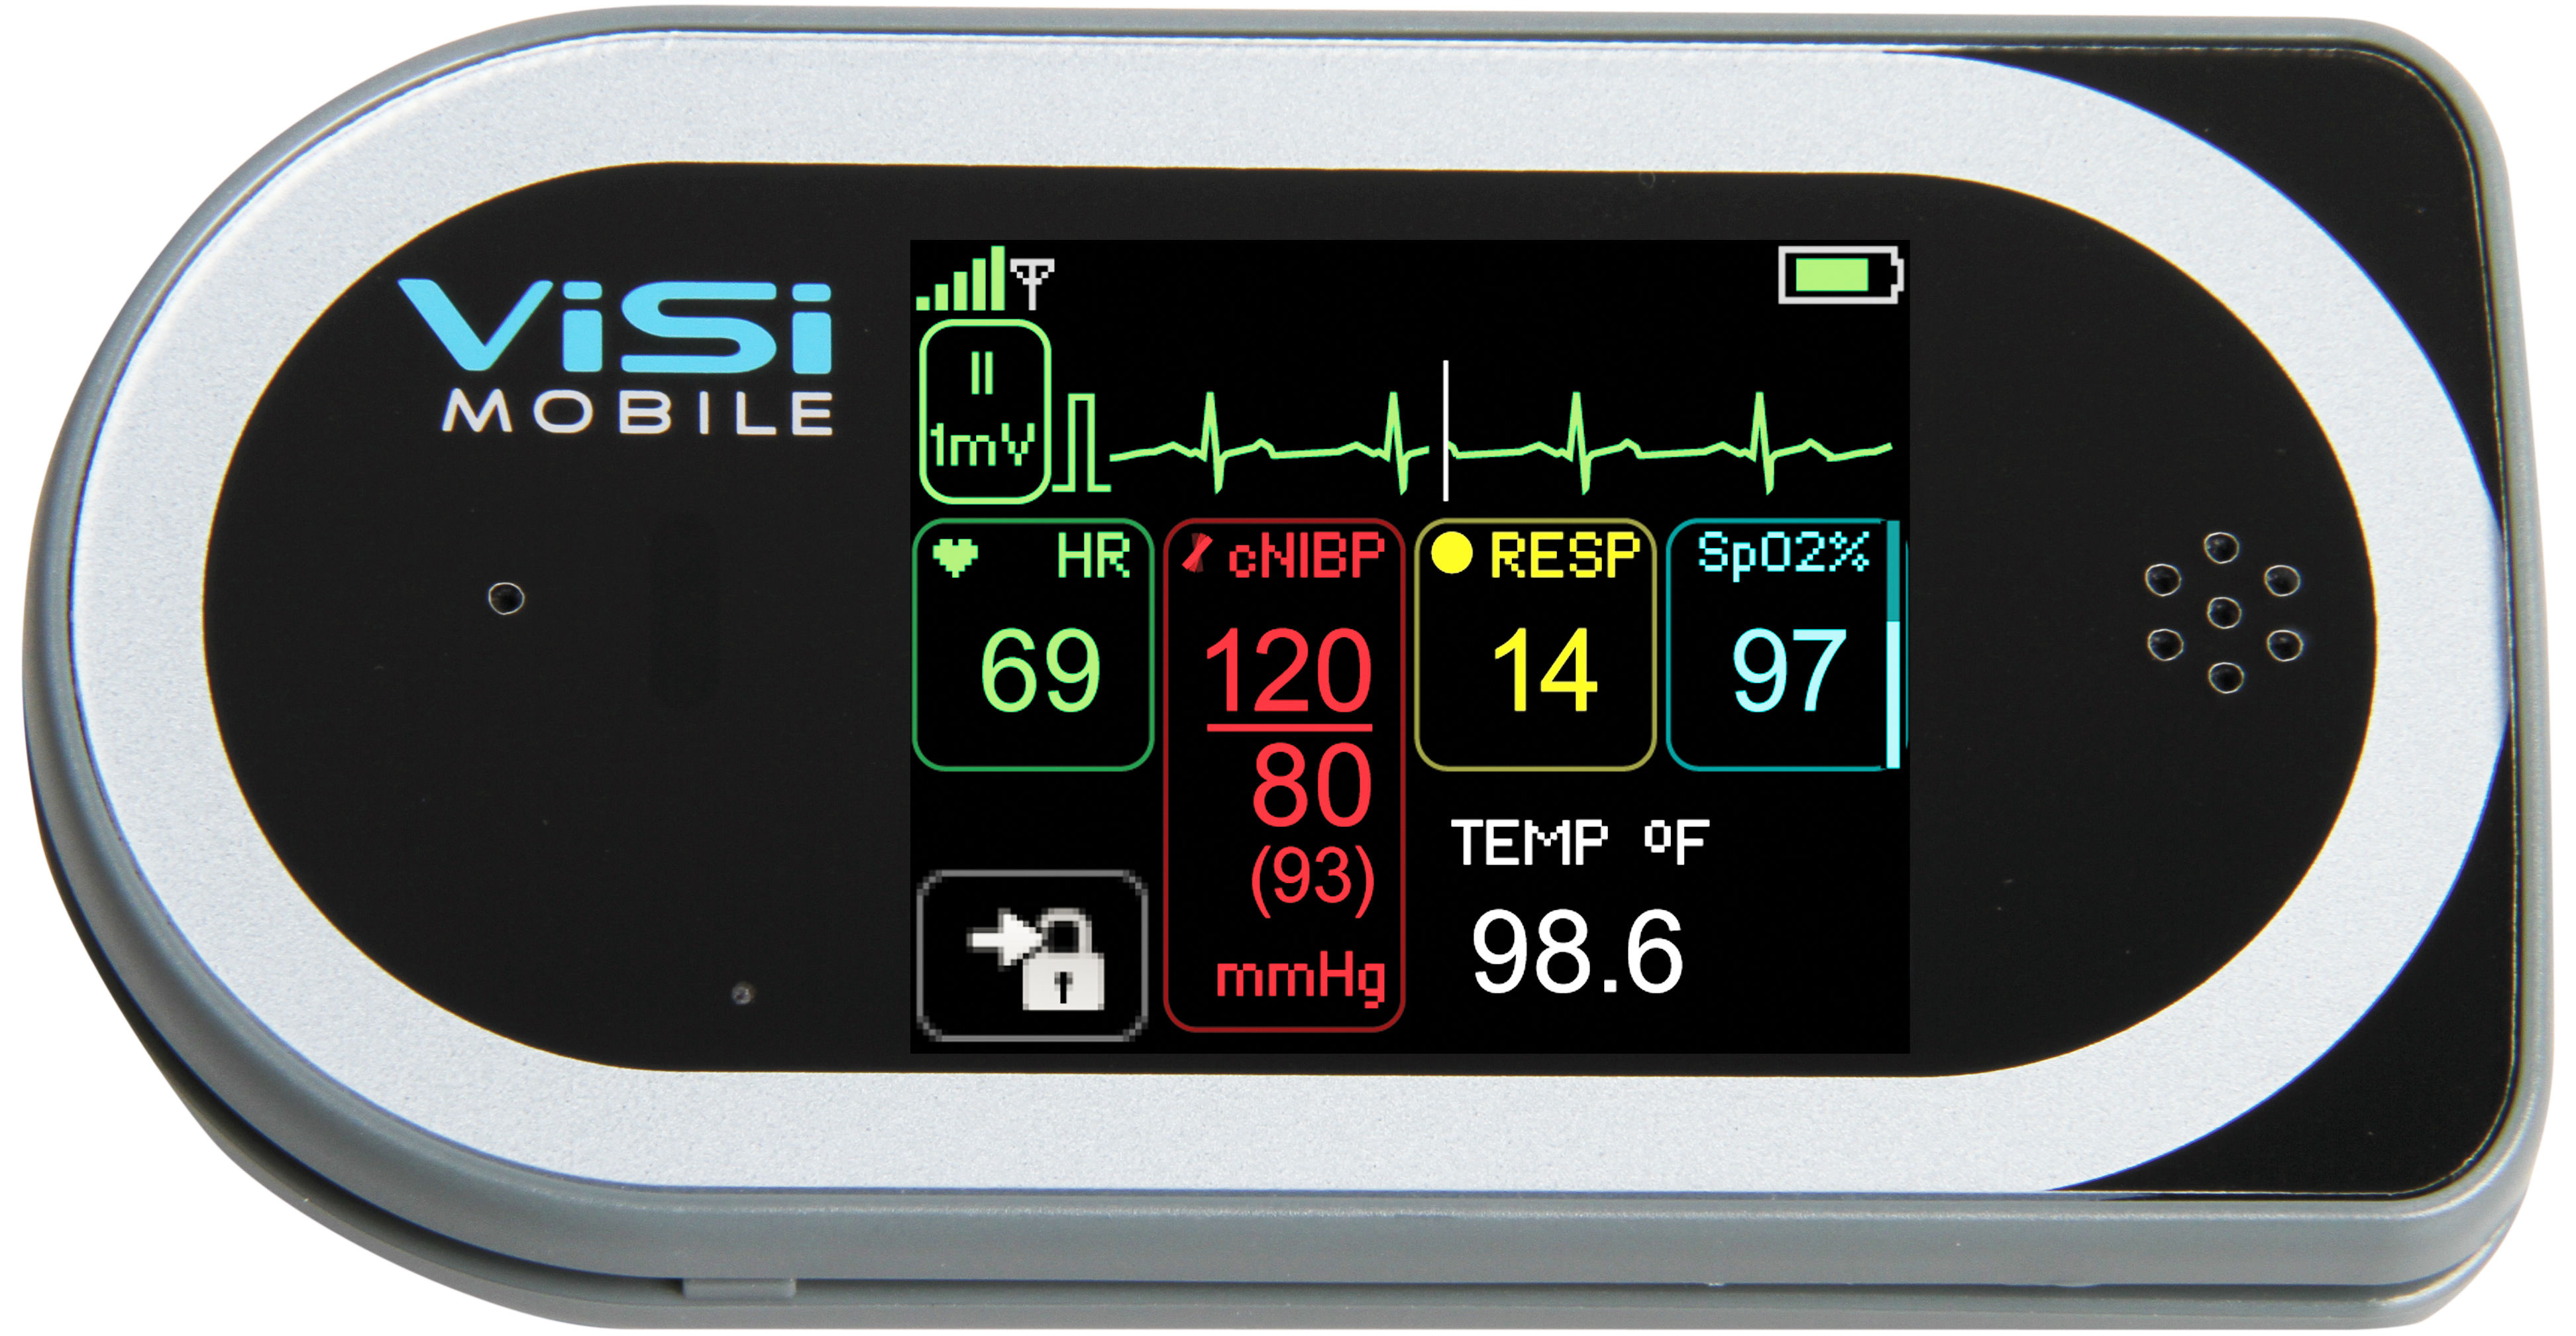
\includegraphics[scale=0.3]{figuras/estadoarte/visi/visi.jpg}
	\caption{Interfaz de usuario ViSi Mobile\textregistered. Fuente: https://es.dotmed.com/}
	\label{visi1}
\end{figure}

Se puede observar en la figura \ref{visi1} la interfaz que puede ver el paciente al utilizar el dispositivo.

\begin{figure}[H]
	\centering
	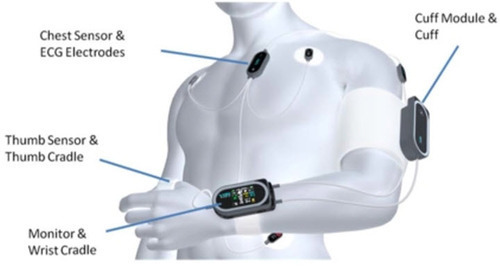
\includegraphics[scale=0.7]{figuras/estadoarte/visi/wear.jpg}
	\caption{Modo de uso ViSi Mobile\textregistered. Fuente: http://www.lasplash.com}
	\label{visi2}
\end{figure}

En la imagen de la figura \ref{visi2}, se puede observar los sensores conectados al cuerpo que convergen al dispositivo que toma las señales.

\section{Qardiocore\textregistered}

QardioCore\textregistered\ \cite{qardio} es un monitor de electrocardiograma inalámbrico diseñado para mejorar la detección y manejo de las condiciones cardíacas. Seis sensores se encargan de grabar y analizar sobre 20 millones de puntos de datos durante todo el día junto con otros signos vitales. Este dispositivo está orientado a personas con alto nivel de riesgo cardíaco causado por predisposición familiar, historial de ataques al corazón, presión alta, colesterol alto, diabetes o exceso de peso. Monitorea de forma precisa y continua la salud del corazón. El dispositivo graba datos de ECG, pulso, variación de pulso, temperatura corporal, ritmo respiratorio y niveles de estrés. A diferencia de los ECG tradicionales, QardioCore no utiliza gel ni cables para monitorear y funciona entre -20ºC y 60ºC. Adicionalmente, es resistente al agua y su batería dura alrededor de un día. Respecto a las especificaciones técnicas, es capaz de funcionar con una frecuencia de 600 muestras por segundo y una resolución de 16 bit, apoyándose en comunicación Bluetooth 4.0 y plataforma exclusiva iOS (9.0 o superior)\cite{qardio_tel}.

\begin{figure}[H]
	\centering
	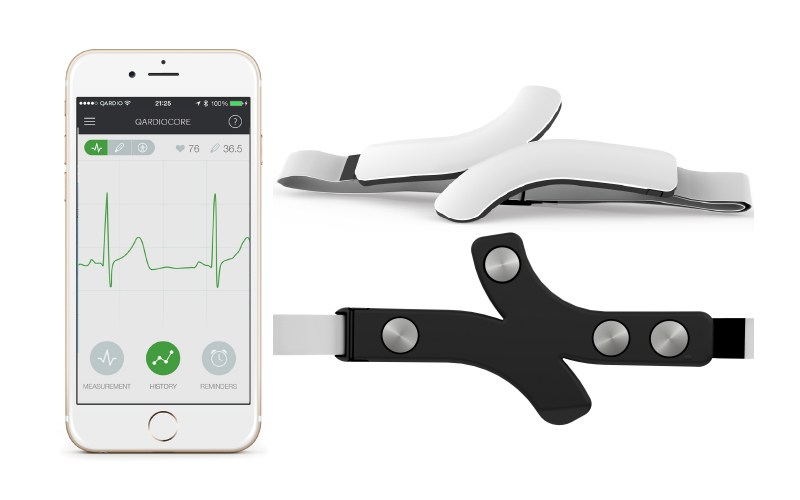
\includegraphics[scale=0.5]{figuras/estadoarte/qardio/qardio.jpg}
	\caption{Qardiocore\textregistered\ multisensor. Fuente: www.fortress.com.hk}
	\label{qardio1}
\end{figure}

Se puede observar el dispositivo Qardiocore en la figura \ref{qardio1} que se conecta a un smartphone para mostrar los datos que se están tomando.

\newpage
Además, como se muestra en la figura \ref{qardio2}, es de simple uso. Funciona como un cinturón en el pecho del paciente.

\begin{figure}[H]
	\centering
	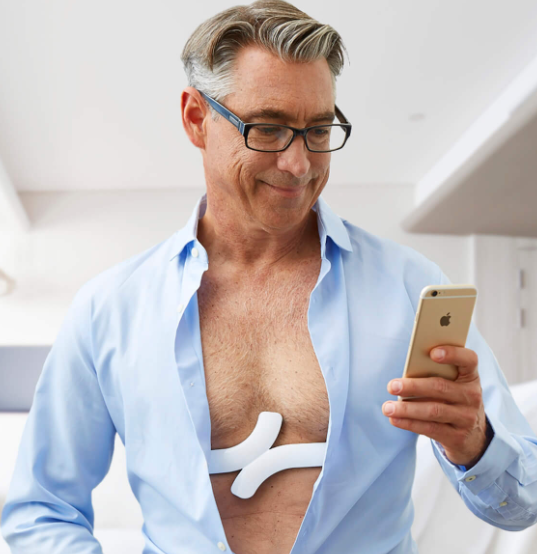
\includegraphics[scale=0.5]{figuras/estadoarte/qardio/wear.png}
	\caption{Modo de uso Qardiocore\textregistered. Fuente: https://www.henleysmed.com}
	\label{qardio2}
\end{figure}

\section{Nuubo\textregistered}

Nuubo\textregistered\ \cite{nuubo} proporciona una nueva perspectiva en la monitorización cardiológica remota e inalámbrica. La plataforma de Nuubo\textregistered\, nECG platform, permite la captura del ECG dinámico a través de un innovador sistema que está basado en textiles biomédicos de nueva generación. Es rentable, remoto, continuo y no invasivo. Además, puede ser utilizado simultáneamente con uno o varios pacientes. Se basa en tecnología Bluetooth v2.0 + EDR (PC y móvil), con una frecuencia de 250 muestras por segundo y 12 bit de resolución\cite{nuubo_tel}.
La tecnología de electrodos textiles desarrollada por Nuubo\textregistered\ simplifica enormemente los incómodos procedimientos tradicionales de conexión de electrodos, reduciéndolos al sencillo acto de vestir la camiseta nECG SHIRT que se muestra en la figura \ref{shirt}.

\begin{figure}[H]
	\centering
	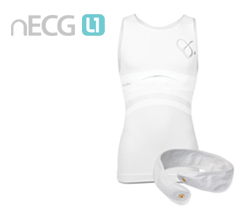
\includegraphics[scale=0.6]{figuras/estadoarte/nuubo/shirt.png}
	\caption{nECG Shirt. Fuente: http://pdf.medicalexpo.es}
	\label{shirt}
\end{figure}

El tejido elástico se adapta a los movimientos del paciente, quien puede realizar su actividad física diaria sin estar limitado por cables y sin necesidad de depender de personal médico especializado. Estas características junto con la información de contexto, la actividad física del paciente y su posición/postura, permite el desarrollo de un nuevo rango de soluciones y casos de uso. 

\begin{figure}[H]
	\centering
	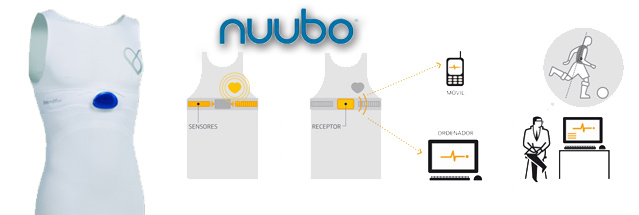
\includegraphics[scale=0.7]{figuras/estadoarte/nuubo/nuubo.png}
	\caption{Sistema Nuubo. Fuente: http://sportics.es}
	\label{nuubo}
\end{figure}

Como se puede observar en la figura \ref{nuubo}, la polera toma los datos que son enviados a un dispositivo movil o un computador para que sea visto por el doctor de manera remota.

%Capítulo 3: Arquitectura de la solución
\newpage
\chapter{Arquitectura de la solución}\label{arquitectura}

Luego de analizar las necesidades del proyecto y el estado actual de la industria frente al desafío, el siguiente paso es establecer una arquitectura base con la cual definir las partes más relevantes del sistema. En la figura \ref{arqui} se pueden apreciar las 3 secciones más importantes y detalladas más adelante. Cabe destacar que es transversal la necesidad de herramientas que permitan un rápido despliegue, con el fin de generar pruebas constantemente.

\begin{figure}[H]
	\centering
	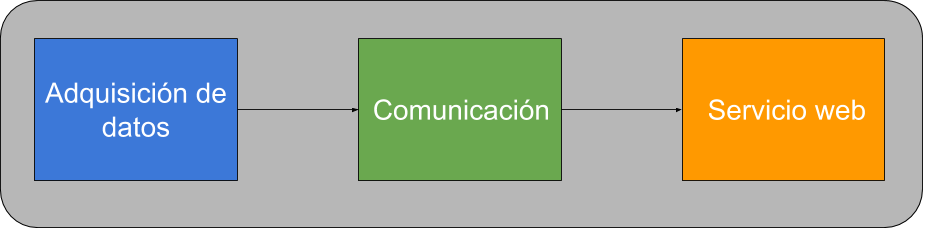
\includegraphics[scale=0.43]{figuras/arquitectura/arqui.png}
	\caption{Arquitectura referente. Fuente: Elaboración propia}
	\label{arqui}
\end{figure}

\newpage
\section{Adquisición de datos}
Una primera necesidad del proyecto es la obtención y procesamiento de los datos, en una primera instancia se omitirá la definición del almacenamiento, permitiendo enfocar los esfuerzos en la selección de sensores, su interconexión y la plataforma que sustente su funcionamiento. Algunos de los requisitos en este apartado son:

\begin{enumerate}
	\item \textbf{Variedad:}
	Considerando la gama de enfermedades que se podrían cubrir, es importante contemplar una plataforma que permita trabajar con gran cantidad sensores.
	\item \textbf{Comodidad:}
	A raíz de que este apartado es el único que tendrá contacto con el paciente es importante pensar en el confort ofrecido, descartando opciones que afecten este apartado, como placas demasiado grandes o pesadas.
	\item \textbf{Flexibilidad:}
	Al estar en un proceso iterativo en búsqueda de opciones, un factor a considerar es la flexibilidad que nos puedan ofrecer las distintas opciones, permitiéndonos realizar cambios importantes sin afectar en gran medida las decisiones ya tomadas.
\end{enumerate}

\newpage
\section{Comunicación}
Dado los requerimientos del proyecto, como lo son las restricciones geográficas que impone Chile y un dispositivo de bajo costo, es necesario contemplar alternativas que no impliquen demasiada infraestructura (o que hagan uso de infraestructura ya disponible) y que además posean la penetración (o el potencial) necesaria dado el territorio nacional. Dentro de las características relevantes en este apartado, podemos encontrar:

\begin{enumerate}
	\item \textbf{Gran cobertura:}
	Considerando la envergadura inicial del proyecto, Chile, es de vital importancia que la tecnología a utilizar permita generar conexiones en la mayor parte del territorio nacional.
	\item \textbf{Alta disponibilidad:}
	Se requiere que la tecnología a emplear permita establecer conexiones a lo largo del tiempo, presentando pocas o de preferencia nulas desconexiones o incapacidades de conexión.
	\item \textbf{Escalabilidad:}
	Si bien es un aspecto dependiente de los anteriores requerimientos, es relevante considerarlo por separado como la medida que representa la capacidad de atender una gran cantidad de conexiones.
\end{enumerate}

\newpage
\section{Servicio web}
El sistema completo requiere además de los puntos anteriores, de un servicio web acorde con las necesidades del proyecto. El cual le de soporte y lo dote de mayores prestaciones, completando así un ecosistema completo en función del desafío. Entre los puntos más relevantes de este apartado se consideran:

\begin{enumerate}
	\item \textbf{Baja latencia:}
	Este proyecto se desarrolla en un marco con pacientes y posibles estados críticos de los mismos, es por ello que el tiempo de respuesta es fundamental en el servicio que se pretende ofrecer.
	\item \textbf{Alta concurrencia}
	Actualmente es común que las conexiones a servicios web tengan una alta demanda y larga duración, aumentando la concurrencia notablemente. Lo anterior es lo que se espera de un monitoreo, el cual debe ser constante en el tiempo (o al menos en una cierta ventana).
	\item \textbf{Seguridad:}
	Los datos que utilizará el sistema son totalmente privados y la protección de estos junto con los datos de conexión son un eje fundamental en la elección de tecnología a emplear, o en su defecto usar capas de seguridad anexas para brindar esta funcionalidad que se considera base.
\end{enumerate}

%Capítulo 4: Alternativas de desarrollo
\newpage
\chapter{Alternativas de desarrollo}\label{alternativas}
En el presente capítulo se ahondará en las distintas alternativas de diseño que existen para el prototipo con los distintos sensores requeridos, además de establecer la comunicación y el envío de la información tomada del paciente. Las etapas para el desarrollo del prototipo constan de: 
\begin{enumerate}
	\item Elección de sistema de procesamiento o unidad central.
	\item Sensores a utilizar.
	\item Forma de comunicación inalámbrica.
\end{enumerate}

\section{Plataforma de desarrollo}\label{proce}
Al fabricar un prototipo, el desarrollador debe construir el hardware sobre el cual correrá el software del producto que ha diseñado, por lo que debe tomar componentes de diversos proveedores, integrarlos y hacerlos funcionar como un conjunto. Por esa razón se popularizó el uso de plataformas de desarrollo electrónico.  \\
Por lo general, estas son placas que integran microcontroladores, circuitos y componentes electrónicos que le proporcionan diversas capacidades básicas, y a partir de esto se puede evaluar la compatibilidad del diseño tanto en hardware como en software antes de enviar a fabricar el producto final. 

\newpage
\subsection{Arduino}
Arduino es una plataforma de desarrollo de bajo costo que permite crear proyectos de base tecnológica de forma sencilla y barata. Que consta de entradas análogas, entradas y salidas digitales, PWM, comunicación serial, etc. 

Uno de los beneficios de Arduino es que provee módulos de desarrollo de bajo costo para trabajar con chips integrados, estudiar su funcionamiento y prototipado.
Arduino trabaja con una gran variedad microcontroladores AVR que diferencia por modelos dependiendo de las necesidades de proyecto, motivo por el cual varía en precio. 

En primera instancia se puede trabajar con un modelo Arduino UNO que es de bajo costo y permite leer señales análogas y traducirlas en su conversor análogo-digital. Dependiendo de las necesidades se puede conseguir otro modelo, como Arduino Mega, que ofrece mayores prestaciones. 
\subsection{Raspberry}
Raspberry es una computadora de placa reducida (SBC por sus siglas en inglés) de bajo costo, con el objetivo de estimular la enseñanza de ciencias de la computación. No obstante, es de propiedad registrada para poder mantener el control de las 8 plataformas disponibles de Raspberry y no se generan excesivas variantes como es el caso de Arduino. El software que usa es open source, aunque es capaz de ejecutar incluso una versión de Windows 10. Por lo mismo su capacidad de procesar señales es mayor y permite ejecutar proyectos más complejos. No se define si es que pueden o no ser usadas en desarrollos comerciales.

\newpage
\subsection{Beaglebone}
Beaglebone black es la última iteración de la serie Beaglebone. Esencialmente es similar a Raspberry, diferenciándose en cosas como la capacidad para iniciarse sin la necesidad de instalar ningún sistema operativo ya que tiene memoria integrada, no así Raspberry. Adicionalmente cuenta con una cantidad de entradas sustancialmente mayor, por lo que permite hasta el doble de conexiones que su competencia directa Raspberry. Como si eso no fuera suficiente, la arquitectura del procesador que incluye Beaglebone black permite que rinda hasta el doble de rápido que su contraparte en Raspberry pi. \\
Al igual que su competencia, Beaglebone ofrece mucho mas procesamiento que el necesario por lo que se descarta como una opción para el desarrollo inicial del prototipo. De acuerdo a las necesidades que vayan surgiendo se puede considerar nuevamente como una opción.
\newpage
\section{Sensores}
A partir de la información que provee la contraparte, se decide que las enfermedades  más comunes son las afecciones cardíacas. También es necesario tener un control de la temperatura de los pacientes a la hora de leer sus signos vitales. \\
Por otra parte se propuso utilizar una IMU para detectar si algún paciente sufre una caída, esto con el fin de emitir una alarma para llamar una ambulancia en caso de ser necesario.
\subsection{ECG}
Electrocardiograma o ECG es el proceso de registrar la actividad eléctrica del corazón en un periodo de tiempo usando electrodos directamente en la piel.\\
Una parte fundamental para el desarrollo de un prototipo será buscar un circuito de desarrollo para realizar una prueba de concepto, en la cual se puedan tomar los datos y manejar.
\subsubsection{DFRobot Heart Rate Monitor Sensor}
El monitor de actividad cardiaca de la empresa DFRobot se usa para medir la actividad electrica del corazón con un chip integrado AD8232\cite{ad8232}, que toma señales análogas de los electrodos y utiliza amplificadores para tener una mejor lectura de los datos.\\
Utilizando un Arduino, es posible leer los datos tomados de los electrodos y convertirlos a información digital que puede ser enviada por comunicación serial.\\

\begin{figure}[H]
	\centering
	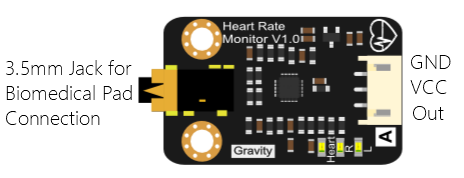
\includegraphics[scale=0.5]{figuras/sensor/ecg/ecg.png}
	\caption{Placa de desarrollo ECG. Fuente: https://circuit.rocks/}
	\label{ecg}
\end{figure}

Como se puede observar en la figura \ref{ecg}, el dispositivo posee conexión simple para electrodos y salida análoga, lo que permitirá una rápida prueba de concepto para utilizar este integrado en el diseño del dispositivo final.


\subsubsection{ADS1298}
El chip integrado ADS1298 de la empresa "Texas Instruments" ofrece un ECG con 8 amplificadores programables de bajo ruido y 8 conversores Análogo-digital de alta resolución.\\
Utilizado para instrumentación medica y lectura tanto de ECG como EMG (Electromiograma) y EEG (Electroencefalograma).\\
El chip integrado ADS1298 es una buena opción para un desarrollo de ECG en el futuro, pero es de un precio 10 veces mayor al dispositivo DFRobot, por lo que se va a descartar para el prototipo funcional.
\subsection{Temperatura}
Cuando se requiere realizar alguna medición a un paciente, siempre es necesario conocer su temperatura corporal. La temperatura sirve como información complementaria, es por esto que se evaluarán termistores que permitan la lectura de este dato.
\subsubsection{Lilypad Temperature Sensor}
Dentro de la tendencia del hardware abierto, uno de los proyectos más destacados es Lilypad Arduino, un conjunto de piezas electrónicas que se pueden coser a los tejidos para darles interactividad con sensores, luces o sonidos.\\
Entre estos sensores tenemos un sensor de temperatura compuesto por un termistor MCP9700 el cual ofrece una resolución de $\pm2^\circ C.$\\

\newpage
La ventjas que ofrece este sensor son el ser de muy bajo costo y a su vez impermeable, por lo que permitiría incorporarlo en el wearable de forma permanente sin dañar la componente.

\begin{figure}[H]
	\centering
	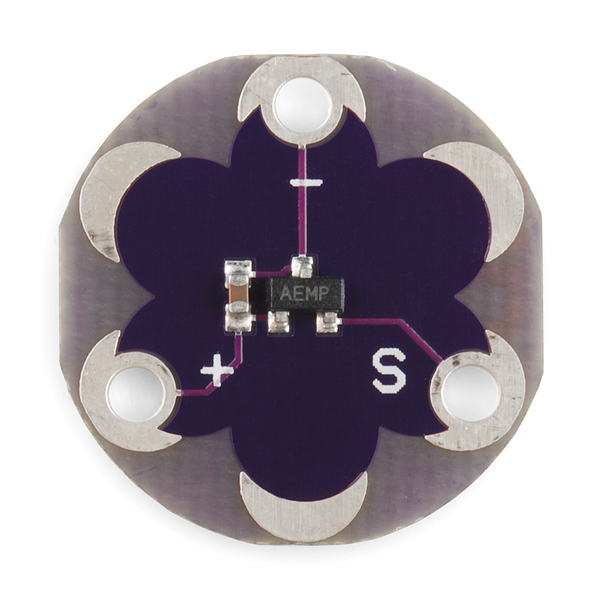
\includegraphics[scale=0.7]{figuras/sensor/t/lilypad.jpg}
	\caption{Sensor de temperatura Lilypad. Fuente: https://www.sparkfun.com/}
	\label{Lilypad}
\end{figure}

Como se puede observar en la figura \ref{Lilypad}, Lilypad ofrece una PCB impermeable con 3 terminales que permiten utilizar un hilo conductor para coser este a la ropa.

\subsubsection{DS18B20}
El sensor DS18B20\cite{temp} es un termómetro digital que ofrece una medida de 9 a 12 bits de resolución. Se comunica mediante el bus 1-Wire lo cual permitiría, en caso de ser necesario, incorporar más sensores para obtener una medida con mayor precisión. 
Este termómetro digital ofrece una resolución de $\pm0.5^\circ C$ y a su vez ofrece un formato impermeable en forma cilíndrica como se observa en la figura \ref{DS18B20}.

\begin{figure}[H]
	\centering
	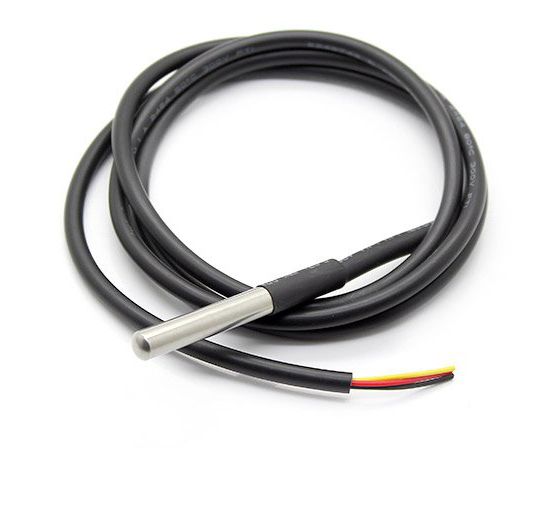
\includegraphics[scale=0.2]{figuras/sensor/t/ds18.jpg}
	\caption{Sensor de temperatura DS18B20. Fuente: https://chips.mecatronium.com/}
	\label{DS18B20}
\end{figure}

\subsection{Ritmo Respiratorio}
Para medir el ritmo respiratorio, se consideró el uso de la tela conductiva MedTex sugerida por la contraparte, la cual entrega un valor de resistividad en ohms en su estado en reposo y este varía dependiendo de su estiramiento.\\

\begin{figure}[H]
	\centering
	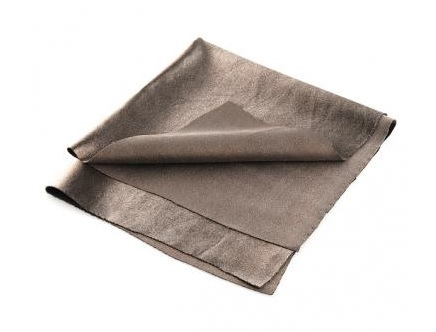
\includegraphics[scale=0.5]{figuras/tela/medtex.jpg}
	\caption{Tela Conductiva MedTex. Fuente: https://es.aliexpress.com/}
	\label{medtex}
\end{figure}

Para estudiar la factibilidad de la tela conductiva que se puede observar en la figura \ref{medtex}, se cortó una tira de un tamaño $20x2 [cm]$ en estiramiento cero sobre una banda elástica que luego fue cosida como cinturón de pecho. Una vez colocada, en cada extremo de la tela conductiva se colocó un caimán conectado a su vez a un multitester que permitía visualizar variaciones de la resistividad de la tela a partir de su estiramiento. 

\newpage
\begin{table}[H]
	\centering
	\begin{tabular}{| c | c | c |}
		\hline
		\multicolumn{1}{|c|}{\textbf{Resistencia en reposo [$\Omega$]}}&
		\multicolumn{1}{c|}{\textbf{Resistencia en estiramiento [$\Omega$]}}&
		\multicolumn{1}{|c|}{\textbf{\% de variación}}\\ \hline
		$4.8$  & $4.6$  & $0.1420$  \\ \hline
		$4.7$  & $4.5$ & $0.1421$ \\ \hline
		$4.8$ & $4.7$  & $0.0722$  \\ \hline
	\end{tabular}
	\caption{Valores resistencia Tela MedTex en Pectorales}
	\label{tablatex1}
\end{table}

\begin{table}[H]
	\centering
	\begin{tabular}{| c | c | c |}
		\hline
		\multicolumn{1}{|c|}{\textbf{Resistencia en reposo [$\Omega$]}}&
		\multicolumn{1}{c|}{\textbf{Resistencia en estiramiento [$\Omega$]}}&
		\multicolumn{1}{|c|}{\textbf{\% de variación}}\\ \hline
		$4.7$  & $4.6$  & $0.0699$  \\ \hline
		$4.7$  & $4.6$ & $0.0699$ \\ \hline
		$4.6$ & $4.5$  & $0.0723$  \\ \hline
	\end{tabular}
	\caption{Valores resistencia Tela MedTex en Plexo}
	\label{tablatex2}
\end{table}

\begin{table}[H]
	\centering
	\begin{tabular}{| c | c | c |}
		\hline
		\multicolumn{1}{|c|}{\textbf{Resistencia en reposo [$\Omega$]}}&
		\multicolumn{1}{c|}{\textbf{Resistencia en estiramiento [$\Omega$]}}&
		\multicolumn{1}{|c|}{\textbf{\% de variación}}\\ \hline
		$4.7$  & $4.6$  & $0.0699$  \\ \hline
		$4.8$  & $4.7$ & $0.0722$ \\ \hline
		$4.7$ & $4.5$  & $0.1421$  \\ \hline
	\end{tabular}
	\caption{Valores resistencia Tela MedTex en Estomago}
	\label{tablatex3}
\end{table}

Se puede observar en las tablas \ref{tablatex1}, \ref{tablatex2} y \ref{tablatex3} que las variaciones de resistencias no son constantes ni regulares, el mismo estiramiento a veces no producía la misma variaciones de resistencia. Además por mínimas variaciones en el movimiento, también habían variaciones que arruinaban la medición, por lo que esta alternativa no sería viable para medir el ritmo respiratorio.

\subsection{Unidad de movimiento inercial (IMU)}
Una unidad de movimiento inercial o IMU (del inglés inertial measurement unit), es un dispositivo electrónico que mide la aceleración, inclinación y las fuerzas gravitacionales, usando una combinación de acelerómetros y giroscopios.
\subsubsection{MPU-9250}
El integrado MPU-9250 es un modulo multi-chip que consiste en 2 chips integrados en un empaquetado QFN. Este provee un giroscopio de 3 ejes y un acelerómetro de 3 ejes.
Este chip provee tres conversores análogo-digital de 16 bits para digitalizar las salidas del giroscopio, acelerómetro y giroscopio de manera independiente.\\
Sparkfun provee una PCB de desarrollo para realizar pruebas como se muestra en la imagen \ref{imu1}.

\begin{figure}[H]
	\centering
	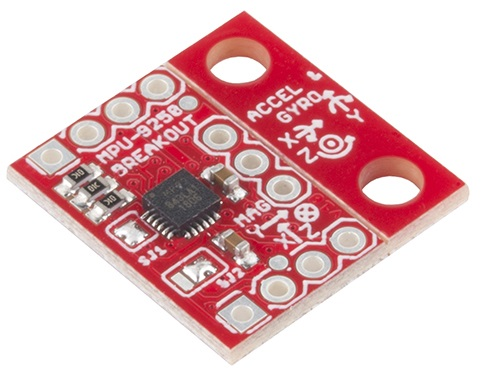
\includegraphics[scale=1.5]{figuras/sensor/imu/imu1.jpg}
	\caption{IMU Sparkfun MPU-9250. Fuente: https://www.sparkfun.com/}
	\label{imu1}
\end{figure}

Es importante destacar la orientación indicada por el fabricante al momento de diseñar el equipo electrónico que son predefinidas como se puede ver en el caso de la figura \ref{imu1} en la cual se muestran los ejes X, Y y Z tanto para el acelerómetro como para el giroscopio. 
\newpage
Como se observa en la figura \ref{imu11} se muestra además de los ejes de aceleración también las coordenadas de navegación (roll, pitch, yaw). 

\begin{figure}[H]
	\centering
	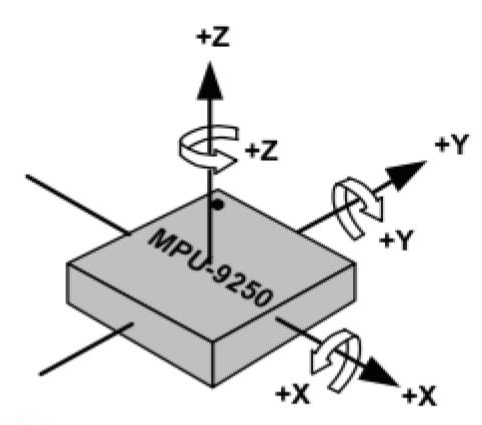
\includegraphics[scale=0.5]{figuras/sensor/imu/imu11.jpg}
	\caption{Ejes IMU MPU-9250. Fuente: https://www.sparkfun.com/}
	\label{imu11}
\end{figure}

\section{Comunicación}
Para el proyecto se consideran distintas alternativas de conexión, las cuales deben seguir ciertos aspectos relevantes según las especificaciones del dispositivo a implementar. 


\begin{enumerate}
	\item \textbf{Alta disponibilidad:}
	Se requiere que la tecnología a emplear permita establecer conexiones a lo largo del tiempo, presentando pocas o de preferencia nulas desconexiones o incapacidades de conexión.
	\item \textbf{Gran cobertura:}
	Considerando la envergadura inicial del proyecto, Chile, es de vital importancia que la tecnología a utilizar permita generar conexiones en la mayor parte del territorio nacional.
	\item \textbf{Bajo costo:}
	Dentro de los requerimientos del proyecto se encuentra el desarrollo e implementación a bajo costo de la solución final, por tanto la tecnología de comunicación a emplear debe seguir esta directriz para ser seleccionada.
	\item \textbf{Baja complejidad:}
	Considerando que el dispositivo en cuestión debiera ser lo más autónomo y sencillo de configurar, es relevante considerar tecnologías de comunicación que no requieran de complejas operaciones para su uso e implementación.
	\item \textbf{Escalabilidad:}
	Si bien es un aspecto dependiente de los anteriores requerimientos, es relevante considerarlo por separado como la medida que representa la capacidad de atender una gran cantidad de conexiones concurrentes (más allá del tiempo de cada conexión).
\end{enumerate}

En base a lo anterior, se hace un análisis rápido de diferentes alternativas que podrían utilizarse en el proyecto:

\begin{enumerate}
	\item \textbf{Antenas de RF:}\cite{RF}
	Comunicación generada en las bandas situadas entre los 3 kilohercios (KHz) y 300 Gigahercios (GHz). Esta tecnología incluye otras como las redes celulares, pero en este apartado se especifica el uso de bandas no utilizadas por esta, permitiendo una conexión directa de antena a antena a una frecuencia específica a determinar.
	
	\item \textbf{Comunicación satelital:}\cite{satelite}
	Comunicación  por medio de ondas electromagnéticas transmitidas gracias a la presencia en el espacio de satélites artificiales situados en órbita alrededor de la Tierra. Dentro de esta tecnología se pueden encontrar dos grandes clasificaciones: 
	\begin{enumerate}
		\item Satélites activos: Satélites que amplifican la señal reenviada a la Tierra.
		\item Satélites pasivos: Satélites que no amplifican la señal reenviada a la Tierra.
	\end{enumerate}
	
	\item \textbf{Redes Wi-Fi:}\cite{wifi}
	También llamada WLAN (Wireless lan, red inalámbrica) o estándar IEEE 802.11, es una de las tecnologías de comunicación inalámbrica mediante ondas más utilizada hoy en día. Existen distintas variantes de este estándar de comunicación, entre los que se destacan 802.11g y 802.11n, por su uso actual en dispositivos comerciales.
	
	\item \textbf{Redes celulares:}\cite{celular}
	Consiste en una red de celdas cada una con su propio transmisor, conocidas como estación base. Ampliamente utilizadas en la actualidad, lográndose encontrar hasta 7 compañías distintas que ofrecen sus servicios en Chile: Movistar, Entel, WOM, Claro, Virgin, VTR, SIMPLE.
	\begin{enumerate}
		\item \textbf{Comunicación directa:}
		Tipo de comunicación en donde el dispositivo posee la capacidad de conectarse, registrarse y hacer uso completo de la infraestructura proporcionada por distintas compañías.
		
		\item \textbf{Comunicación indirecta:}
		Tipo de comunicación con la cual el dispositivo requiere de un paso intermedio de comunicación para generar la conexión a la red requerida, para este paso se puede destacar el uso de Bluetooth para la comunicación con otro dispositivo con la capacidad de conectarse de forma directa a las redes celulares.
	\end{enumerate}	
\end{enumerate}	

Luego de caracterizar las distintas tecnologías disponibles para su uso en el proyecto, se procede a analizar sus cualidades en función de las 4 especificaciones anteriores: 

\begin{table}[H]
	\centering
	\begin{tabular}{| c | c | c | c | c | c |}
		\hline
		\multicolumn{1}{|c|}{\textbf{Tecnología}}&
		\multicolumn{1}{c|}{\textbf{Disponibilidad}}&
		\multicolumn{1}{|c|}{\textbf{Cobertura}}&
		\multicolumn{1}{|c|}{\textbf{Costo}}&
		\multicolumn{1}{|c|}{\textbf{Complejidad}}&
		\multicolumn{1}{|c|}{\textbf{Escalable}}\\ \hline
		Antenas RF  & Alta  & Baja & Alta & Alta & Baja \\ \hline
		Satelital  & Alta & Alta & Alta & Alta & Baja\\ \hline
		Wi-Fi & Alta & Baja  & Bajo & Media & Alta\\ \hline
		Directa & Alta  & Alta  & Medio & Baja & Alta\\ \hline
		Indirecta & Alta  & Alta/Baja & Bajo & Media & Alta/Media\\ \hline
	\end{tabular}
	\caption{Comparativa tecnologías / requerimientos}
	\label{tablacompara_telecomunicaciones}
\end{table}

A raíz de lo anterior se destaca el uso de tecnologías con redes celulares por su lineamiento con el proyecto. La tecnología Wi-Fi se descarta por ser de baja cobertura (en una primera instancia y pensando a nivel nacional) y esto a su vez ser un ámbito crítico para el proyecto. A continuación se presentan alternativas para la plataforma Arduino en torno a las tecnologías ya mencionadas.

\subsection{Celular directa: GPRS/GSM shield}
Para integrar conexión a redes celulares en el dispositivo es necesario considerar un GPRS shield compatible con socket xbee.\\ GPRSBee cumple con los requerimientos a un precio no menor (aproximadamente 36.000 CLP). 
Se puede observar en la figura \ref{gprs} el módulo disponible para desarrollo.

\begin{figure}[H]
	\centering
	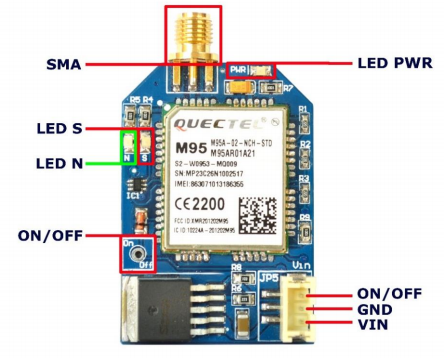
\includegraphics[scale=0.8]{figuras/com/gprs.png}
	\caption{Modulo GPRSBee. Fuente: https://www.mcielectronics.cl/}
	\label{gprs}
\end{figure}

Cabe destacar que para poder utilizar este módulo es necesario incluir una antena que se puede ver en la figura \ref{antena}

\begin{figure}[H]
	\centering
	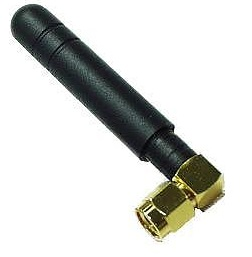
\includegraphics[scale=0.5]{figuras/com/antena.jpg}
	\caption{Antena GPRSBee. Fuente: https://www.mcielectronics.cl/}
	\label{antena}
\end{figure}

Al considerar este módulo, se puede concluir que es incompatible con el diseño del wearable ya que la antena es muy grande (aproximadamente $57.40[mm]$), lo que sería molesto en el dispositivo final. Otro punto en contra de este módulo es el alto costo y el consumo energía que lo hace incompatible con la autonomía que se desea.

\subsection{Celular indirecta: Bluetooth BLE shield}
Para integrar Bluetooth en el dispositivo se considera un BLEBee, el cual ofrece Bluetooth versión 4.1 y comunicación UART mediante un puerto XBEE. \\
El shield Bluetooth posee un módulo RN4020\cite{RN4020} el cual ofrece una antena para la comunicación en su misma placa lo que facilita el diseño, como se puede observar en la figura \ref{bt}.

\begin{figure}[H]
	\centering
	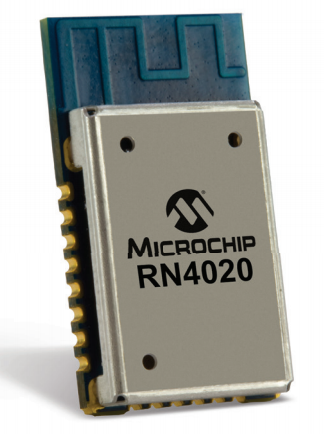
\includegraphics[scale=0.5]{figuras/com/rn4020.png}
	\caption{Bluetooth RN4020. Fuente: https://www.mcielectronics.cl/}
	\label{bt}
\end{figure}

Es importante destacar que para mejorar el diseño, el fabricante recomienda dejar expuesta la antena y se destaca la comunicación UART para las configuraciones futuras del sistema.

\newpage

\section{Conclusiones}
En esta sección, tomando en cuenta las opciones vistas en el mismo capítulo, se seleccionarán las primeras componentes a utilizar para el prototipo funcional y para realizar la prueba de concepto con lo que se va a basar el proyecto.
\subsection{Plataforma de desarrollo}
Para la plataforma de desarrollo se va a escoger trabajar con Arduino ya que este posee distintas versiones con distintos costos, los cuales son menores que Raspberry o Beaglebone. Además, cabe destacar que el sistema que se quiere desarrollar es toma de datos y envío de información, por lo que no se va a requerir tanto procesamiento. Arduino cubre las necesidades en su versión UNO con un microcontrolador ATMega328p y en caso de necesitar uno de mayor capacidad, se puede optar por un Arduino Mega.
\subsection{Electrocardiograma}
Para el sensor de electrocardiograma se utilizará el monitor de actividad cardíaca de DFRobot, esto debido a que es la única opción que se puede conseguir en el país para no retrasar el desarrollo. Este sensor es de muy bajo costo (alrededor de 19.500 CLP en MCIElectronics).
El chip integrado ADS1298 es una buena opción como una mejora para una segunda iteración del diseño para mejorar la señal que se puede obtener debido a que este posee mayor tolerancia al ruido. Se debe descartar esta última opción debido a que se debe encargar directamente desde "Texas Instruments" y esto puede tomar mucho tiempo.

\newpage
\subsection{Temperatura}
En primera instancia se va a utilizar el sensor Lilypad ya que este está diseñado específicamente para wearables. Además, utiliza un hilo conductor para unir sus terminales con la alimentación y la toma de datos. Este sensor tiene un valor aproximado de 3.790 CLP.\\
Dependiendo de los resultados obtenidos en la primeras pruebas, se va a evaluar la segunda alternativa de utilizar el DS18B20, el cual tiene un valor aproximado de 5.900 CLP.
\subsection{IMU}
Al buscar las alternativas que existen en el país, todas las opciones usan distintas placas de desarrollo, pero utilizan el mismo sensor MPU-9250. Dado lo anterior, se va a utilizar la placa de Sparkfun MPU-9250 luego de tener el prototipo funcional con los primeros sensores de electrocardiograma y temperatura. Esta placa de desarrollo tiene un valor aproximado de 12.500 CLP.
\subsection{Comunicación}
Entre las alternativas mencionadas, se opta por utilizar en primera instancia el GPRS/GSM shield, el cual posee un costo aproximado de 43.980 CLP.
Cabe mencionar que en una segunda instancia se utilizaría el chip RN4020, el cual posee un precio aproximado de 20.000 CLP.\\
Si bien el costo es menor, es relevante la complejidad que agrega la segunda opción (al agregar un actor como lo puede ser un teléfono inteligente), además de aumentar los tiempos de respuesta por el actor extra. Es por lo anterior, que se decide en una primera instancia recurrir al módulo GPRS/GSM.

Aunque la flexibilidad que brinda la segunda opción (chip Bluetooth RN4020) y ciertos aspectos negativos de la primera son las que obligan un posterior cambio.

%Capítulo 5: Sistema de telecomunicaciones
\newpage
\chapter{Sistema de telecomunicaciones}\label{comunicacion}
Se determinó utilizar la plataforma Arduino por su simplicidad en prototipado y programación, además de ser de fácil acceso y una tecnología escalable. En base a esto se decide comenzar a trabajar en el apartado de comunicación.
\section{Redes móviles, Bluetooth y Android}
Como se comentó anteriormente, la primera elección de tecnología para la comunicación fue la de utilizar redes móviles directamente, esto por medio del módulo GPRS Shield. Este es un módulo de comunicación 2G compatible con socket XBee para la Arduino UNO (un socket XBee dota a una placa Arduino de la capacidad de comunicarse en forma inalámbrica \cite{xbee_info}). Por agilidad de desarrollo se escogió una variante de Arduino UNO llamado PICARO+, la cual posee entre otras modificaciones el socket XBee integrado.\\
Así, se hace uso tanto de la placa principal, el chip de comunicación y una antena. Estas últimas 2 mencionadas en las figuras \ref{gprs} y \ref{antena}.\\
Dentro de las características del GPRS se encuentran el emplear una tarjeta SIM, conector SMA y el chip Quectel M95. En cuanto a la antena nos encontramos con cuatri-banda: 
\begin{enumerate}
	\item\textbf{GSM/850E: 824 a 894 [MHz]}
	\item\textbf{GSM: 880 a 960 [MHz]}
	\item\textbf{DCS: 1710 a 1880 [MHz]}
	\item\textbf{PCS: 1850 a 1990 [MHz]}
\end{enumerate}

\newpage
Si bien puede parecer cuestionable el utilizar tecnología 2G, es importante considerar que el chip provee de hasta 85.6 [kbps] y diversos protocolos de comunicación. Con lo cual al año 2017 (se espera deshabilitar las redes 2G en el mediano plazo para dar paso a nuevas tecnologías) sirve como prueba de concepto dado su bajo costo y el acercamiento que ofrece a los comandos AT, los cuales son los empleados para controlar chips de este tipo.
Luego de comenzado el proceso de configuración, se encontraron diversos problemas con esta elección:

\begin{enumerate}
	\item\textbf{Dimensiones:}
	Dado que este módulo esta contemplado para operar en conjunto con la placa principal, se hace engorroso el tener una antena de casi 6 [cm] y de gran grosor adosado al cuerpo del paciente.
	\item\textbf{Consumo energético:}
	Este módulo hace necesario el uso de una fuente de alimentación externa de mayor capacidad (9[V] aproximadamente) respecto a la necesidad base de la placa (3.3[V]), lo que conlleva a usar un cargador externo y en su momento a una batería de mayor capacidad.
	\item\textbf{Antigüedad de comandos:}
	Los comandos Hayes (también llamados AT \cite{AT}) son un conjunto de comandos empleados en la configuración y parametrización de módems, su uso data de al menos 1990 y en cierto punto dejaron de usarse para dar paso a controladores específicos. 
	\item\textbf{Tasas de transferencias:}
	A raíz de un estudio preliminar en tasas de transferencia se estableció que alrededor de 150 datos por segundo debían ser enviados (esto en función de las tasas de operación de un ECG común\cite{ecg_rate}), por tanto el usar esta tecnología obliga a emplear 3G como mínimo. 
	\item\textbf{Costo:}
	En comparación a otras tecnologías indirectas de redes móviles como lo puede ser el Bluetooth, la inversión necesaria es mayor y su flexibilidad bastante menor.
\end{enumerate}

Por todo lo anterior, se pasa a una segunda iteración en busca de emplear tecnología Bluetooth y un intermediario para llegar a las redes celulares.\\


\section{Perfiles Bluetooth}

Bluetooth \cite{bluetooth} es una especificación industrial para Redes Inalámbricas de Área Personal (WPAN) creado por Bluetooth Special Interest Group, Inc. que posibilita la transmisión de voz y datos entre diferentes dispositivos mediante un enlace por radiofrecuencia en la banda ISM de los 2.4 GHz, data de 1994 y actualmente se encuentra en su versión 5.0. La versión a emplear en este proyecto es la 4.0 llamada BLE (Bluetooth Low Energy). \\

Un perfil Bluetooth es la especificación de una interfaz de alto nivel para su uso entre dispositivos Bluetooth. 
Los perfiles son descripciones de comportamientos generales que los dispositivos pueden utilizar para comunicarse, formalizados para favorecer un uso unificado. La forma de utilizar las capacidades de Bluetooth se basa, por tanto, en los perfiles que soporta cada dispositivo. Los perfiles permiten la manufactura de dispositivos que se adapten a sus necesidades.\\

A la fecha existen más de 27 perfiles Bluetooth, pero durante el desarrollo del proyecto se emplearon solo dos: SPP y GATT.

Las principales diferencias entre estos últimos dos perfiles son: 
\begin{enumerate}
	\item GATT pertenece al estándar introducido en la versión 4.0 (desde ahora BLE) mientras que SPP en la versión 2.1. 
	\item BLE está pensado para operar con un consumo energético inferior que versiones anteriores, posee mayor velocidad en el establecimiento de la conexión y está pensado para la transferencia de pequeñas cantidades de datos. 
\end{enumerate}
Excepto por el último punto se puede observar una notoria superioridad de GATT (BLE) frente a SPP, pero como se verá más adelante, las tasas de transferencias obtenidas con GATT son lo suficientemente buenas como para escogerla en este proyecto.

\newpage
\section{Razones para elegir Android}

Para seleccionar el intermediario entre la comunicación Bluetooth y las redes móviles se decidió usar un teléfono inteligente por:
\begin{enumerate}
	\item Capacidades de cómputo.
	\item Gran presencia en el mercado de los móviles.
	\item Flexibilidad al ofrecer un entorno de desarrollo propio de su sistema operativo. 
\end{enumerate}
Ahora bien, para seleccionar el sistema operativo se recurre a su penetración en el mercado y como se puede observar en la figura \ref{market_share}, Android se alza como el gigante en el mercado.

\begin{figure}[H]
	\centering
	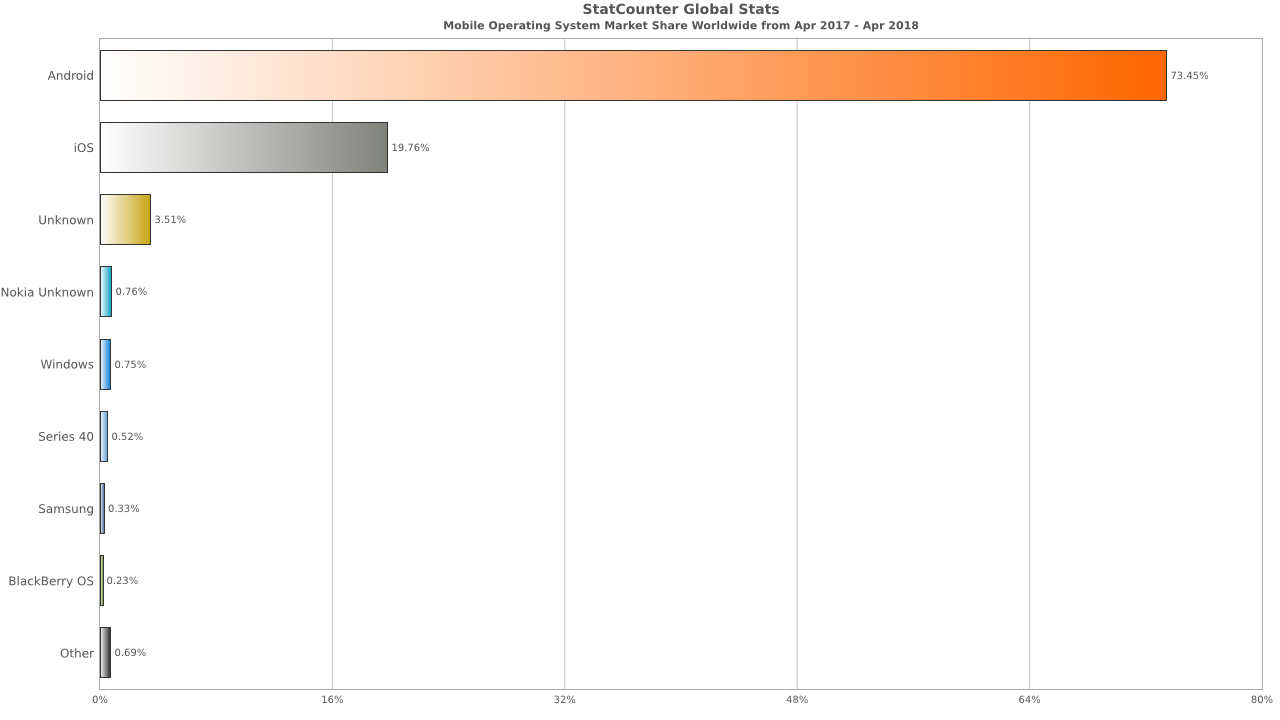
\includegraphics[scale=0.4]{figuras/comunicacion/Market_share.png}
	\caption{Mercado compartido mundial de sistemas operativos móviles 2017-2018 \cite{market_share_cita}}
	\label{market_share}
\end{figure}

Además de lo anterior, se ha de considerar el entorno de desarrollo y el ecosistema que rodea al sistema operativo en cuestión. En el caso de Android, se trabaja principalmente con Android Studio (Para sistemas Linux, Windows y Mac), en lenguaje Java o Kotlin, con una comunidad activa de desarrolladores y una gran cantidad de librerías a disposición.\\
Por último se considera la accesibilidad de los terminales, con lo cual es de conocimiento general que Apple posee precios más elevados que los dispositivos Android.
Por lo tanto se concluye que Android es la mejor alternativa en estos momentos.

\newpage
\section{Comparativa desarrollo híbrido}
Para el desarrollo móvil actual existen dos grandes aproximaciones, las cuales pasan principalmente por el uso de entornos de desarrollo que permiten el despliegue en más de un sistema operativo (llamados híbridos) o uno determinado con un solo código fuente.\\

Primero, en el ámbito nativo (un código fuente para un despliegue único): 

\begin{table}[H]
	\centering
	\begin{tabular}{| c | c | c | c |}
		\hline
		\multicolumn{1}{|c|}{\textbf{OS}}&
		\multicolumn{1}{c|}{\textbf{Lenguaje}}&
		\multicolumn{1}{|c|}{\textbf{IDE}}&
		\multicolumn{1}{|c|}{\textbf{Plataforma}}\\ \hline
		Android  & Java, Kotlin  & Android Studio, Eclipse & Linux, Mac, Windows \\ \hline
		iOS  & Objective-C, Swift & XCode & Mac \\ \hline
	\end{tabular}
	\caption{Comparativa de desarrollo nativo, elaboración propia}
	\label{native_comparative}
\end{table}

Continuando con el ámbito híbrido, se destacan 3 grandes competidores:

\begin{table}[H]
	\centering
	\begin{tabular}{| c | c | c |}
		\hline
		\multicolumn{1}{|c|}{\textbf{Framework}}&
		\multicolumn{1}{c|}{\textbf{Tipo de resultado}}&
		\multicolumn{1}{|c|}{\textbf{Lenguaje}}\\ \hline
		Ionic  & No nativo  & JavaScript (AngularJS) \\ \hline
		Reac Native  & Nativo & JavaScript (React) \\ \hline
		Flutter  & Nativo & Dart \\ \hline
	\end{tabular}
	\caption{Comparativa de desarrollo híbrido, elaboración propia}
	\label{hybrid_comparative}
\end{table}

Por último se analizan ventajas y desventajas de ambas aproximaciones al desarrollo móvil, cabe destacar que Flutter aún en 2018 se encuentra en fase beta, pero se considera por las grandes prestaciones que presenta (por lo que no se considerarán sus ventajas en la siguiente tabla), además se establece un marco en donde se espera obtener un desarrollo tanto para iOS como para Android:

\begin{table}[H]
	\centering
	\begin{tabular}{| c | c | c |}
		\hline
		\multicolumn{1}{|c|}{\textbf{Característica}}&
		\multicolumn{1}{c|}{\textbf{Nativo}}&
		\multicolumn{1}{|c|}{\textbf{Híbrido}}\\ \hline
		Rendimiento  & Máximo  & Suficiente \\ \hline
		Actualizaciones SO  & Sin retraso & Con retraso \\ \hline
		Librerías  & Extenso & Acotado \\ \hline
		Control  & Total & Parcial \\ \hline
		Tiempo de desarrollo  & Alto & Medio/bajo \\ \hline
		Cantidad de código  & Alto & Mínimo \\ \hline
		Diversidad de código  & Total & Unificado \\ \hline
		Complejidad  & Alta & Baja \\ \hline
	\end{tabular}
	\caption{Desarrollo nativo versus híbrido, elaboración propia}
	\label{native_hybrid}
\end{table}

Como se puede observar en la tabla \ref{native_hybrid}, el mayor potencial para el desarrollo híbrido es cuando no se tienen funcionalidades demasiado específicas (que requieran librerías especiales), no se requiere gran rendimiento, no se utilizarán las últimas características de seguridad del SO y el tiempo es primordial.\\
Si bien se podría considerar el uso híbrido, se espera que la aplicación haga uso de alto poder de procesamiento, utilice librerías específicas (como graficar en tiempo real como se verá más adelante) y se tenga el mayor control posible de todos los procesos. Por lo tanto se descarta el uso de entornos híbridos para el desarrollo, en desmedro de la compatibilidad con dispositivos Apple.


\newpage
\section{Prueba de concepto}

Para comenzar el desarrollo e iniciar los sucesivos Sprint (metodología SCRUM), se hizo uso del perfil SPP de Bluetooth, incluído en su versión 2.1 + EDR (2004) y que permite comunicación bidireccional. Es uno de los perfiles fundamentales de Bluetooth al tener un comportamiento muy parecido a los de la comunicación serial (como la usada en conexiones RS-232 o UART).
Está basado en el protocolo RFCOMM y emula una linea serial, para su uso se utilizan dos actores, uno que actúa como servidor y otro que actúa como cliente. El primero queda a la espera de alguna conexión entrante (visible), luego por medio de una búsqueda y el uso de un UUID el segundo genera una conexión para comenzar a intercambiar datos.

El objetivo es generar una prueba de concepto por el cual se usara a una aplicación Android como puente para llevar información internet.

Para esto se implementó la siguiente arquitectura:

\begin{figure}[H]
	\centering
	
\includegraphics[scale=0.4]{figuras/comunicacion/prueba.png}
	\caption{Arquitectura de la prueba de concepto. Fuente: Elaboración propia}
	\label{prueba_concept}
\end{figure}

Como se puede observar en la figura \ref{prueba_concept} el servidor Bluetooth (desarrollado en Java) fue implementado en un computador con Windows 7, mientras que la aplicación Android básica permite el escaneo, selección y conexión con el servidor Bluetooth. Esto último sin utilizar librerías externas.

La prueba resultó exitosa, pudiendo enviar información (cadenas de texto) desde el computador hasta una página web previamente configurada, la cual se detallará en el siguiente capítulo. Cabe destacar que el uso de este perfil Bluetooth fue solo por simplicidad y próximamente se hará uso de un perfil acorde al proyecto.

%Capítulo 6: Implementación de la solución de lado del servidor
\newpage
\chapter{Implementación de la solución de lado del servidor}\label{servidor}
Los microcontroladores Arduino son usados en el diseño de sistemas embebidos para distintas funciones. El microcontrolador es un pequeño chip que posee pines con funciones de lectura y escritura, memoria, entradas y salidas. Mientras los microcontroladores han sido usados por décadas, los microcontroladores Arduino son utilizados actualmente ya que permiten ejecutar funciones electrónicas sin necesidad de conocer hardware y software integrado en estos. 
\section{Bootloader}
Dentro de las múltiples definiciones que existen con respecto al bootloader, lo más común es considerarlo como un software o firmware que reside parcialmente en la memoria no volátil del microcontrolador, como la ROM o memoria Flash. \\
En la práctica el bootloader empieza a funcionar justo después de prender el microcontrolador o después de reiniciarlo. \\
Este bootloader va a ser el que va a permitir la programación del circuito con el entorno de desarrollo Arduino (Arduino IDE) manejando de mejor manera la toma de datos por medio de las entradas análogas, el procesamiento y la comunicación.

\newpage
\section{ISP - In-System Programming}
También conocido como programación serial en circuito\cite{isp} (ICSP), es la habilidad de algunos dispositivos lógicos programables, microcontroladores y otros circuitos electrónicos de ser programados mientras están instalados en un sistema completo, no es necesario programar el chip antes de instalarlo en el sistema. Esto permite armar un circuito con todo lo que se desea y programarlo en el circuito impreso.\\
Típicamente los chips que soportan programación ISP tienen circuitería interna que genera el voltaje necesario y permite comunicarse con el programador a través de protocolo serial.
La mayoría de los dispositivos lógicos programables usan una variante del protocolo JTAG para ISP para facilitar la integración con procedimientos automatizados de pruebas.\\
JTAG (Joint Test Action Group) es una interfaz diseñada originalmente para circuitos impresos y es muy útil también como mecanismo para depuración de aplicaciones embebidas, puesto que provee una puerta trasera para acceder al sistema. El módulo de depuración permite al programador corregir errores de código y de lógica de sus sistemas.\\

\begin{figure}[H]
\centering
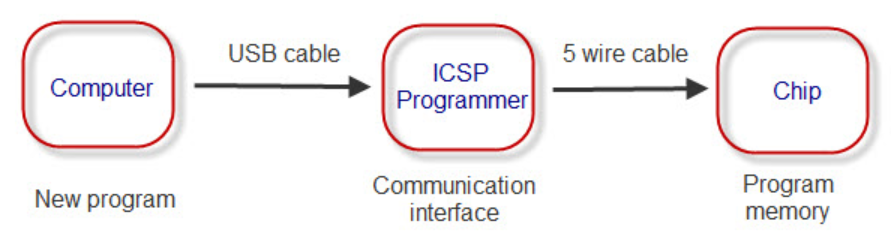
\includegraphics[scale=0.5]{figuras/firmware/isp.png}
\caption{Configuración ISP para programar un microcontrolador}
\label{isp}
\end{figure}

Se observa en la Figura \ref{isp} un simple diagrama de flujo donde es importante destacar que para poder programar un chip es necesaria una conexión de 5 cables entre un intermediario que viene a ser el programador ICSP (o ISP) y el chip (Microcontrolador).

\newpage
\section{Programación de un microcontrolador}
Para que el entorno de desarrollo Arduino reconozca el microcontrolador como una placa Arduino, es necesario grabar el bootloader en este. Se escribe el bootloader en la memoria del microcontrolador mediante la comunicación ISP que se muestra en la figura \ref{pin}.

\begin{figure}[H]
\centering
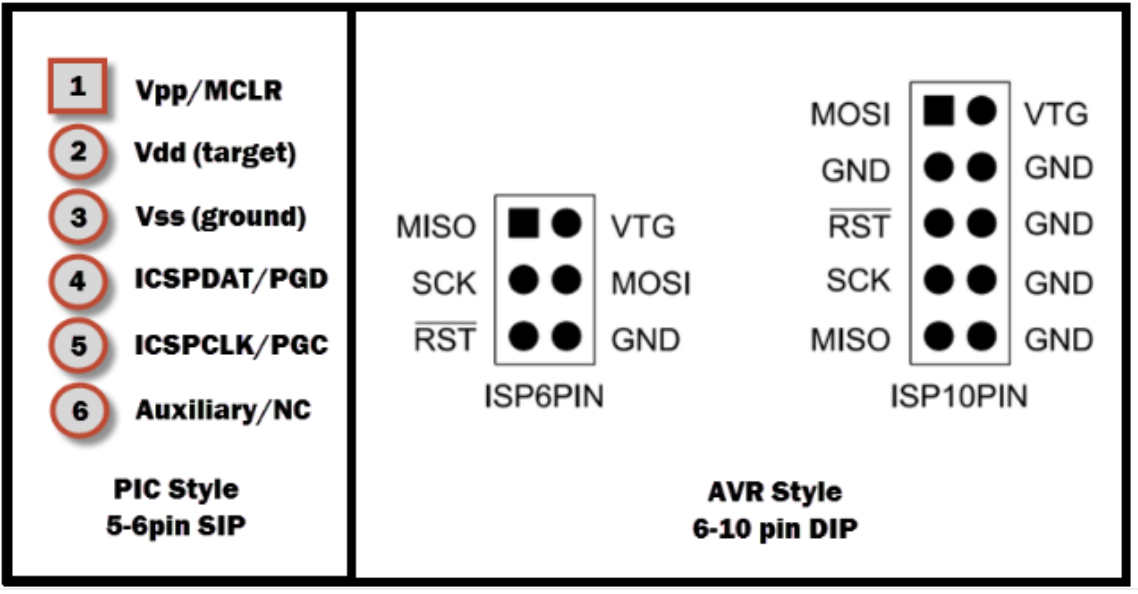
\includegraphics[scale=0.5]{figuras/firmware/pin.png}
\caption{Conector típico para programación ISP}
\label{pin}
\end{figure}

La figura \ref{pin} muestra el conector ISP que se va a encargar de cargar el bootloader en el microcontrolador.  En este caso se está utilizando la tecnología AVR (microcontrolador ATMega) la cual es usada por las placas Arduino y es por esto que se usará la configuración de 6 pines. 

\begin{figure}[H]
\centering
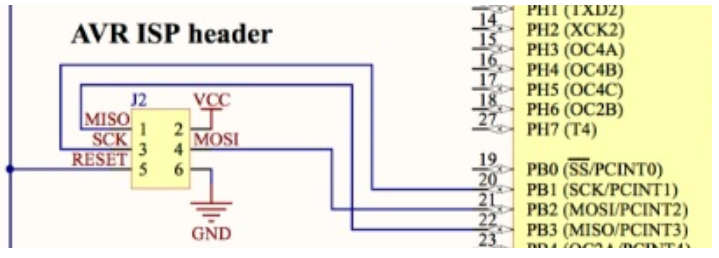
\includegraphics[scale=0.6]{figuras/firmware/eagleisp.png}
\caption{Esquemático básico MCU con ISP}
\label{eagle11}
\end{figure}

En la figura \ref{eagle11} se muestra una parte del esquemático con la configuración básica en el microcontrolador AVR.
Se puede observar el diagrama de conexión del bus con el microcontrolador. Esto se puede observar con mayor detalle en la tabla \ref{tablaisp}\\

\subsection{Programador ISP}
 Existen varias alternativas que cumplen esta función y dependen tanto del microcontrolador como del fabricante. Un microcontrolador AVR (Atmel) requiere de un programador STK500 con una interfaz serial RS232 (Existen otros programadores pero cumplen la misma función, el STK500 es el más utilizado y posee mayor compatibilidad). Para programar un microcontrolador de Microchip se requiere de un PICkit.\\ 
Una segunda alternativa es utilizar un Arduino ya programada que cumpla la función del programador. Estas vienen con un puerto ISP el cual permite cargar el bootloader en el microcontrolador. Respetando la misma conexión que se muestra en la figura \ref{eagle11}.\\

\begin{table}[H]
\centering
\begin{tabular}{| c | c | c |}
\hline
\multicolumn{1}{|c|}{\textbf{AVR ISP}}&
\multicolumn{1}{c|}{\textbf{Arduino UNO}}&
\multicolumn{1}{|c|}{\textbf{ATMega2560}}\\ \hline
1 & MISO  & Pin 22 \\ \hline
2 & VCC   & VCC    \\ \hline
3 & SCK   & PIN 20 \\ \hline
4 & MOSI  & Pin 21 \\ \hline
5 & RESET & Pin 30 \\ \hline
6 & GND   & GND    \\ \hline
\end{tabular}
\caption{Programación ISP utilizando Arduino UNO}
\label{tablaisp}
\end{table}

\section{Programación USB}
La compañía escocesa Future Technology Devices International (FTDI) está especializada en la tecnología USB (Universal Serial Bus). Esta ofrece chips encargados de transformar una conexión USB a un puerto UART y esto será fundamental a la hora de programar el diseño final con el programa en el entorno Arduino.
\newpage
\subsection{FT232RL}
El Chip FT232RL\cite{ft232} ofrece una conversión USB-UART y cuenta con 28 pines como se muestra en la figura \ref{ft232ft}.

\begin{figure}[H]
\centering
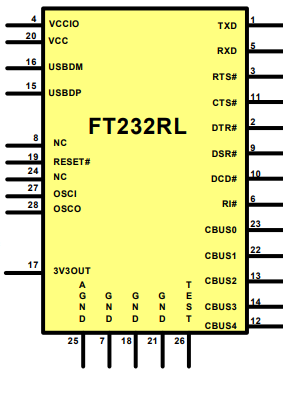
\includegraphics[scale=0.6]{figuras/firmware/ft232.png}
\caption{Chip FT232RL}
\label{ft232ft}
\end{figure}

En la tabla \ref{ft232} se muestra la descripción de los pines más importantes para la conexión del FTDI con el microcontrolador y al mismo tiempo con el USB para permitir la programación del chip. 

\begin{table}[H]
\centering
\begin{tabular}{| c | c | c | c |}
\hline
\multicolumn{1}{|c|}{\textbf{Nº Pin}}&
\multicolumn{1}{c|}{\textbf{Nombre}}&
\multicolumn{1}{|c|}{\textbf{Descripción}}\\ \hline
1  & TXD    & Transmisor de datos UART \\ \hline
5  & RXD    & Receptor de datos UART    \\ \hline
4  & VCCIO  & 1.8[V] a 5.25[V] alimentación a la interfaz UART y a los pines CBUS \\ \hline
15 & USBDP  & Conexión Data+ USB \\ \hline
16 & USBDM  & Conexión Data- USB \\ \hline
17 & 3V3OUT & Regulador de voltaje interno.    \\ \hline
22 & CBUS1  & Indicador de funcionamiento RXD   \\ \hline
23 & CBUS2  & Indicador de funcionamiento TXD    \\ \hline
\end{tabular}
\caption{Descripción de pines chip FT232RL}
\label{ft232}
\end{table}

Este chip será encargado de conectar la interfaz UART (TX y RX) con el microcontrolador además de permitir la comunicación con la conexión USB (USBDP y USBDM).\\
Al trabajar con una conexión USB se tiene conexión con VCC y GND desde el computador que está programando y este provee una alimentación de 5[V]. Este voltaje es comúnmente utilizado en los microcontroladores pero además provee un regulador de voltaje interno de 3.3[V] el cual está disponible si se está trabajando con un sistema con menor voltaje.
En caso de utilizar voltaje 3.3[V] para todo el sistema, es necesario conectar el pin 3V3OUT a VCCIO utilizando un condensador de 100[nF] como se indica en el manual. De esta forma la alimentación del microcontrolador es la misma que la alimentación FTDI para la programación UART y no se dañan las componentes.

\begin{figure}[H]
\centering
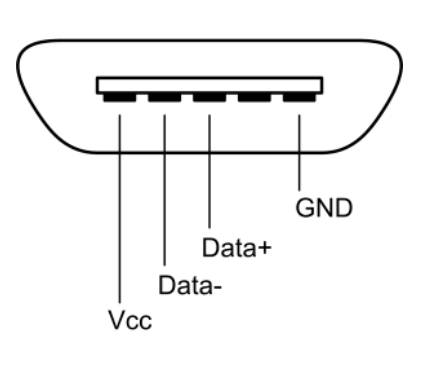
\includegraphics[scale=0.6]{figuras/firmware/usb.png}
\caption{Conector USB 2.0 Micro B}
\label{usb}
\end{figure}

Se muestra en la figura \ref{usb} las 4 conexiones que posee un conector USB, las cuales son la alimentación VCC, GND y la conexión de datos Data+ (USBDP en FT232) y Data- (USBDM en FT232). 

\newpage
\section{Programa en Arduino}

Para la programación del Arduino se trabajó en conjunto con la parte telemática del grupo. Se realizó la programación de la toma de datos de los sensores. Además de un algoritmo antirebote para pedir toma de muestras en el prototipo que luego fue sustituido por una orden emitida por la aplicación. Este código se puede observar en el anexo. En esta parte se puede observar la división de las tareas en el grupo debido a que esta memoria está enfocada al area de diseño de hardware mayoritariamente por lo que este código no se explicará en mayor profundidad.

%Capítulo 7: Implementación de la solución de lado del cliente Android
\newpage
\chapter{Implementación de la solución de lado del cliente Android}\label{servicios}
En este capitulo se van a juntar las partes diseñadas anteriormente para obtener un esquemático final que será adaptado a una PCB utilizando el programa EagleCAD. Además se diseñará un botón ON/OFF con el objetivo de no utilizar interruptores de 2 o mas posiciones.
\section{Botón ON/OFF}
Con las nuevas tecnologías van quedando obsoletos los botones o interruptores de 2 posiciones como se puede observar un ejemplo en la figura \ref{toggle} y también causado por la disminución del tamaño de los dispositivos electrónicos. 

\begin{figure}[H]
\centering
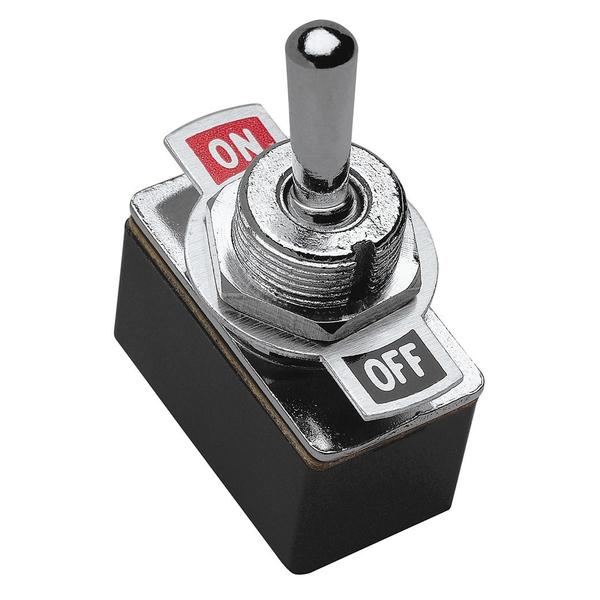
\includegraphics[scale=0.15]{figuras/eagle/toggle.png}
\caption{Interruptor de 2 posiciones}
\label{toggle}
\end{figure}

Estos interruptores ofrecen la funcionalidad que se necesita para un prototipo pero es necesario diseñar un dispositivo final para entregar al cliente. Es por esto nace el requerimiento de que se deba usar un botón único para encender y apagar el dispositivo y esto no es una tarea trivial.\\
	Los requerimientos para este botón es que baje a $0[V]$ cuando se apaga, que sea un único botón y que no requiere ninguna programación. \\

Un circuito muy utilizado que cumple los requerimientos anteriores se puede observar en la figura \ref{esquematico}.\\

\begin{figure}[H]
\centering
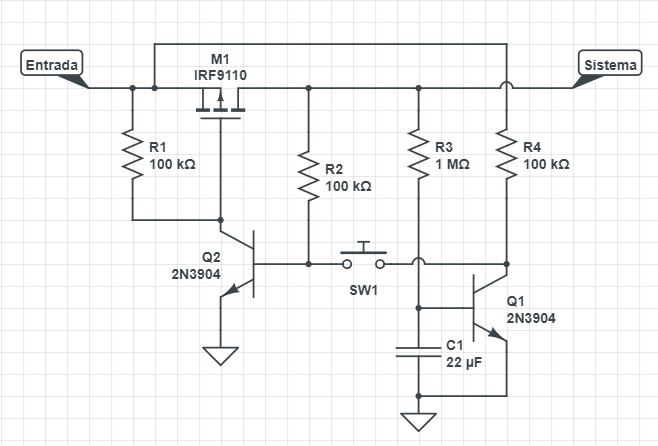
\includegraphics[scale=0.7]{figuras/eagle/circuito.png}
\caption{Circuito para botón ON/OFF}
\label{esquematico}
\end{figure}

Este circuito cumple con los requerimientos de ser simple, funcionar con un solo botón que cumple ambas funciones de encendido y apagado. \\
Alimentando el circuito con una entrada de $3[V]$ cuando se presiona el botón para encender, se alimenta la base del transistor Q2 lo que provoca que el mosfet M1 permita el paso de la corriente desde ''Drain'' hasta ''Source'' esto va a permitir que se alimente el sistema, además va a alimentar el transistor Q1 lo que va a permitir cargar el condensador C1.\\
El condensador C1 es utilizado para mantener alimentado el transistor Q1 ya que al presionar el botón, una persona normal podría demorar entre $0.1[s]$ a $0.5[s]$ en todo el proceso ya que es humano, por lo que se utiliza para cargarlo en ese tiempo y no se apague automáticamente al soltar el botón.\\
En una segunda etapa cuando se pulsa el botón para apagar, se corta la base del transistor Q2 y utilizando la resistencia equivalente del Arduino el condensador se va a descargar pasando la corriente hacia el sistema y finalmente se cortará la alimentación.\\
Probando este circuito con un osciloscopio se puede corroborar el funcionamiento de encendido y apagado como se muestra en la figura  \ref{on}

\begin{figure}[H]
\centering
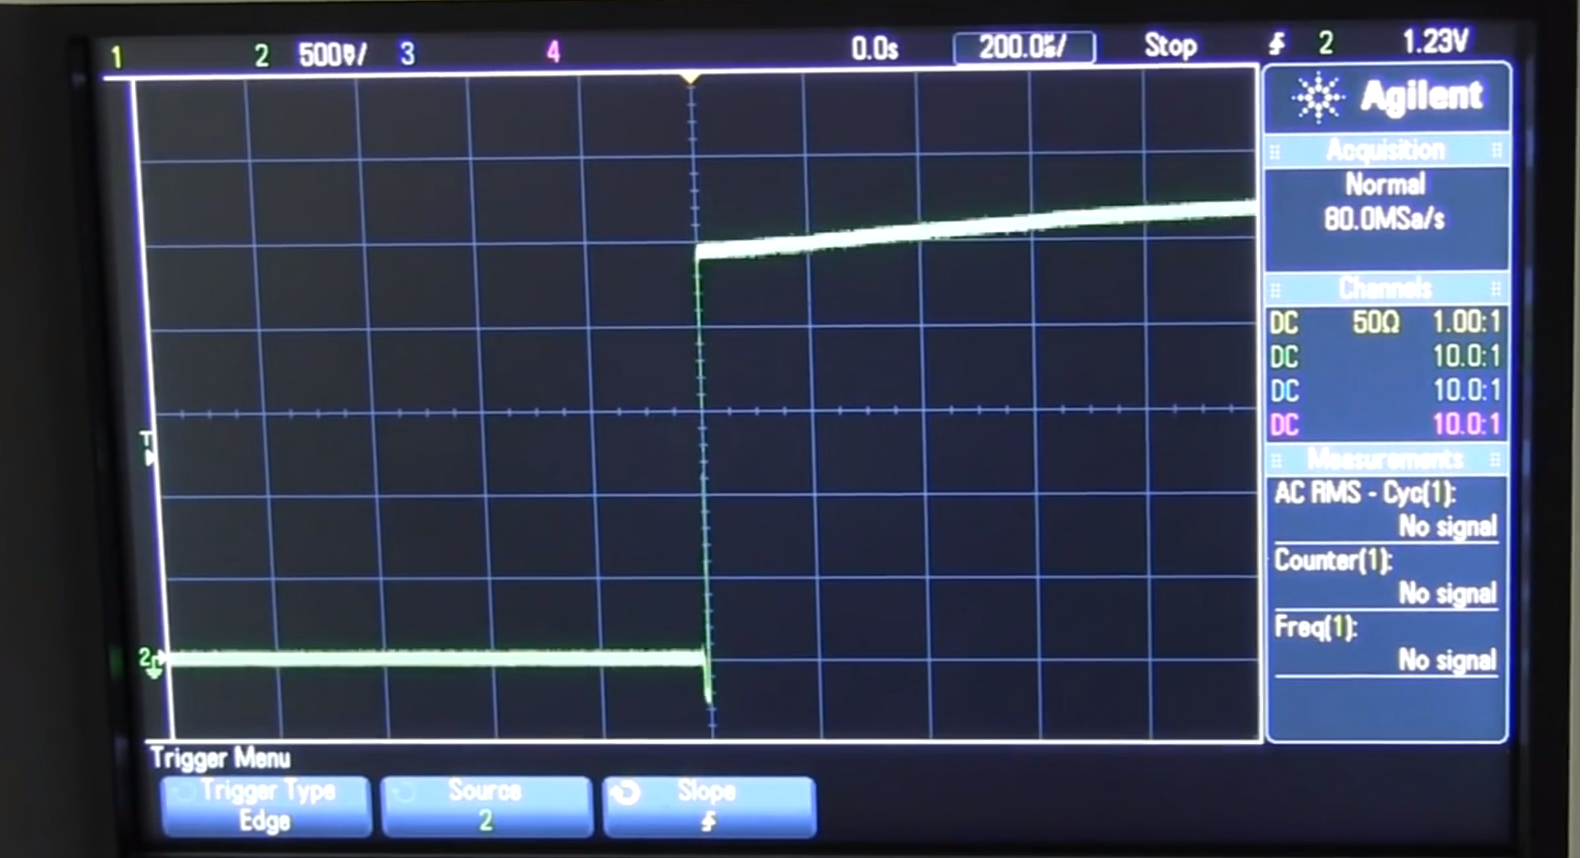
\includegraphics[scale=0.23]{figuras/eagle/on.png}
\caption{Función de encendido}
\label{on}
\end{figure}

Esto muestra lo poco que demora el circuito en pasar de un estado a otro y permite mantenerse encendido.

\begin{figure}[H]
\centering
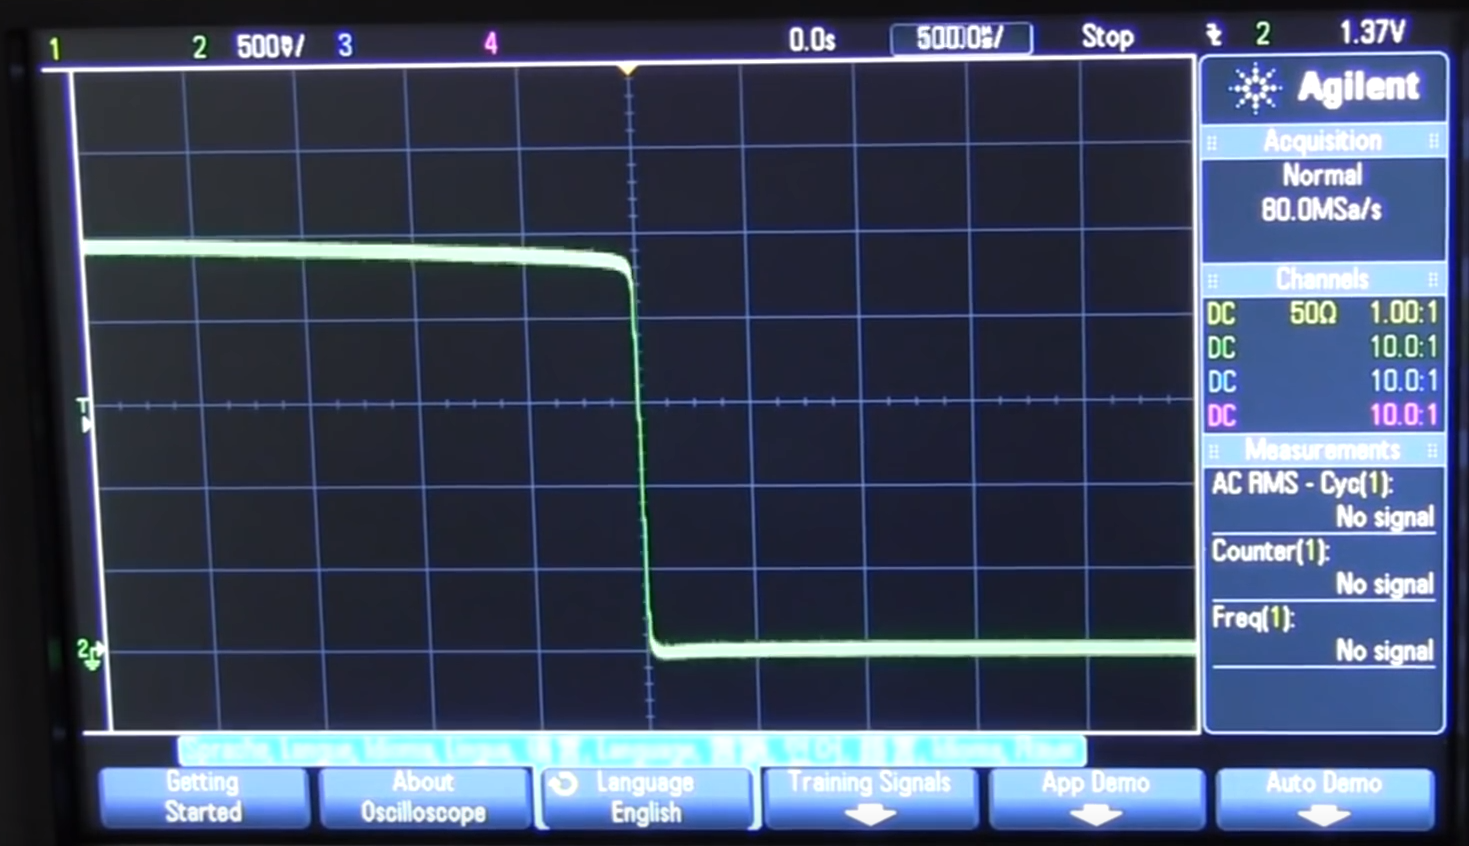
\includegraphics[scale=0.23]{figuras/eagle/off.png}
\caption{Función de apagado}
\label{off}
\end{figure}

En la figura \ref{off} se puede observar que también se demora poco tiempo en descargarse, debido a que está conectado a una carga muy grande y que pide mucha corriente, lo que hace que el tiempo de descarga del condensador C1 sea mucho menor. 

\section{Esquemático}
El diseño final dispositivo se puede considerar como 7 módulos en conjunto entre los cuales se encuentra el microcontrolador, ECG, cargador de batería, botón ON/OFF, FTDI, Bluetooth y regulador de voltaje los cuales resultan en un esquemático final que se puede observar en los anexos.\\
Los módulos mas grandes se explicaron en los capítulos anteriores, en esta sección se explicará el regulador de voltaje y los diseños finales para el dispositivo.
\subsection{Regulador de voltaje 3.3[V]}
Para proveer energía al microcontrolador y al sistema entero, es necesario un regulador de voltaje de bajo ruido que cumpla la función de evitar grandes variaciones que pueden provocar fallas en la PCB.\\
Todos los integrados utilizados tienen un rango aceptable de funcionamiento que varía entre los $2-5[V]$ aproximadamente. En este intervalo los valores comúnmente utilizados son $3.3[V]$ y $5[V]$.\\
La alimentación es un factor determinante a la hora de diseñar un microcontrolador ya que al utilizar un resonador para sincronizar su reloj, dependiendo del voltaje que se provee, este funciona a distintas velocidades como se puede observar en la figura \ref{atmega}.\\

\begin{figure}[H]
\centering
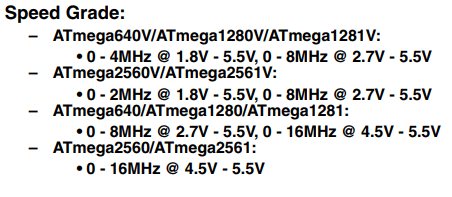
\includegraphics[scale=0.7]{figuras/eagle/atmega.png}
\caption{Velocidades y voltajes recomendados para un microcontrolador ATMega2560}
\label{atmega}
\end{figure}

Como se puede observar, es posible configurar el microcontrolador de $2[MHz]$ con voltaje entre $1.8[V]$ y $5.5[V]$. Además una velocidad de $8[MHz]$ se puede conseguir con un voltaje entre $2.7$ y $5.5[V]$. Finalmente se puede utilizar una velocidad de $16[MHz]$ con un voltaje entre $4.5[V]$ y $5.5[V]$.\\
Como una de las condiciones es que el dispositivo sea de pequeño tamaño y peso, se utilizará una batería de $4.3[V]$ de $950[mAh]$ y es por esto que se va a bajar la velocidad a $8[MHz]$ para utilizar una alimentación de $3.3[V]$.\\

Se utilizará un integrado MIC5219 el cual ofrece un regulador de bajo ruido que funciona a $3.3[V]$ y permitirá energizar el dispositivo. En la figura \ref{reg} se puede observar el integrado y su configuración típica.

\begin{figure}[H]
\centering
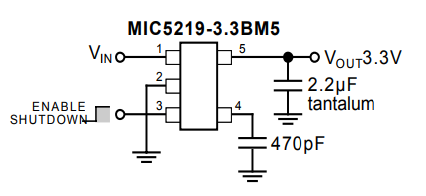
\includegraphics[scale=1]{figuras/eagle/reg.png}
\caption{Regulador de voltaje 3.3[V]}
\label{reg}
\end{figure}

Para entender este diagrama es necesario destacar $V_{in}$ que viene a ser la alimentación de la batería de Li-ion, $V_{out}$ es la salida de $3.3[V]$ hacia la carga que involucra el microcontrolador y todas las componentes del sistema.\\
El pin 2 es la tierra del sistema y el pin 3 ofrece una función para habilitar y deshabilitar el regulador la cual no se va a utilizar. Finalmente el pin 4 ofrece reducción de ruido conectandolo a tierra con un condensador de $470[pF]$.

\subsection{Conector para sensores}
Al trabajar con sensores, es necesario facilitar la tarea para el diseñador de producto de conectar las entradas al sistema con el vestible, es por esto que se va a reducir todos los sensores a un solo conector. Para esto, considerando que se utilizará el ECG y 2 sensores de temperatura para promediar su valor y obtener mayor precisión, se necesitan 5 conectores para los datos y además alimentación y tierra.\\

\begin{figure}[H]
\centering
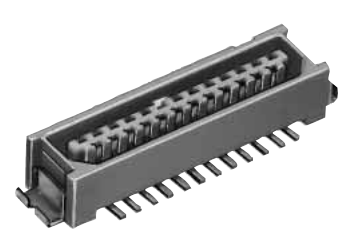
\includegraphics[scale=0.5]{figuras/eagle/conn.png}
\caption{Conector para sensores}
\label{conector}
\end{figure}

El conector que se utilizará se puede observar en la figura \ref{conector}. La particularidad que ofrecen estos tipos de conectores es que poseen entre 9 y 51 contactos.\\
Para el diseño se van utilizar 9 contactos los cuales constan de 3 conectores para los 3 electrodos de ECG, 2 para sensores de temperatura y 4 de alimentación (Voltaje y tierra para ECG independientes de la alimentación de los sensores de temperatura) como se puede observar en la figura \ref{coneagle}.

\begin{figure}[H]
\centering
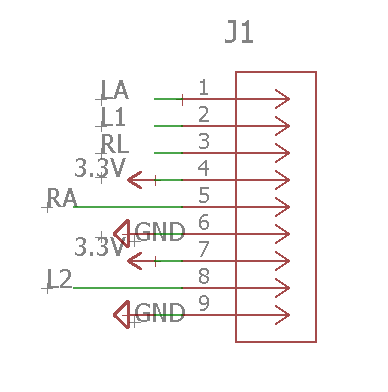
\includegraphics[scale=0.5]{figuras/eagle/sensores.png}
\caption{Conector de 9 pines}
\label{coneagle}
\end{figure}

\subsection{Pin header para prototipo}
Finalmente, como el microcontrolador ofrece 16 pines análogos, 54 digitales y 14 PWM se dejarán headers en la primera iteración del dispositivo para que se pueda seguir prototipando y agregar mas sensores en el futuro, donde se pueda trabajar en el mismo dispositivo en vez de utilizar uno independiente. \\
También se va a dejar disponible pines para comunicación UART (2 utilizadas en el dispositivo y 2 libres) y también los pines SDA y SCL para comunicación I2C. \\

\begin{figure}[H]
\centering
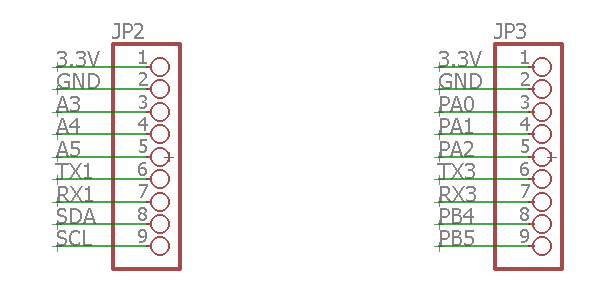
\includegraphics[scale=0.5]{figuras/eagle/header.png}
\caption{Conección Headers}
\label{header}
\end{figure}

Como se puede notar en la figura \ref{header} estos pines ofreceran alimentación y comunicación UART en cada header. 3 pines analogos (A3, A4 y A5), los 2 pines de conección I2C (SDA y SCL) y 5 pines digitales (PA0, PA1, PA2, PB4 y PB5).







%Capítulo 8: Configuración RN4020
\newpage
\chapter{Configuración RN4020}\label{rn4020}

\section{BLE (Bluetooth 4.0)}

El módulo de comunicación consiste en el chip RN4020 de MicroChip, el cual opera bajo el estándar BLE (Bluetooth Low Energy). La tecnología BLE consiste en un nuevo estándar de Bluetooth a partir de su versión 4.0, en la cual se optimiza el tamaño y consumo de potencia de los dispositivos, dentro de su implementación cabe mencionar distintos actores y definiciones con los cuales opera:\newline

	-GAP (Generic Access Profile): Dentro de la GAP se definen varios tipos de roles, pero estos están implementados bajo el concepto en que los dispositivos BLE pueden actuar con rol Central o un rol Periférico. Los dispositivos con rol periférico son pequeños, de baja potencia y que pueden conectarse a un dispositivo central mucho más potente. Los dispositivos periféricos pueden ser: monitor de frecuencia cardíaca, una tarjeta de proximidad BLE, etc. Por lo general, los dispositivos con rol Central usualmente son teléfono móvil, tableta o PC los cuales poseen mucha más potencia de procesamiento y memoria.
	
	-GATT (Generic Attribute Profile): Define de qué modo dos dispositivos Bluetooth de bajo consumo transfieren sus datos, haciendo usos de los conceptos de Servicios y Características. Además se hace uso de un protocolo de datos genéricos llamados Attribute Protocol (ATT) en el cual se almacenan los servicio, características y datos relacionados en una simple tabla de consultas en cuya entrada se utiliza un ID de 16 bits. Una vez que ya se encuentra establecida la comunicación entre los dos dispositivos, entra en juego los servicios y atributos definidos por GATT, es decir, que ya tuvo que haber concluido la etapa de Anuncio y asociación de los dispositivos gobernado por las definiciones establecidas por GAP. Cabe mencionar que los servicios y características descritas en la GATT, la conexión entre el dispositivo periférico y el central es exclusiva, es decir, que solo puede haber una comunicación a la vez. De esta manera, para que otro dispositivo pueda conectarse al periférico, primero debe desconectarse de su enlace actual.
	
	-Anunciación de un dispositivo: Hay dos modos diferentes de realizar el envío de datos en un anuncio GAP : Advertising Data y Scan Response. Los datos enviados en cada uno de los anuncios forman el llamado Payload del mensaje. Ambas cargas son idénticas y pueden almacenar hasta 31 bytes de datos, pero sólo los mensajes de
	advertising son obligatorios para la norma, ya que ésta contiene siempre la información útil que constantemente se está transmitiendo desde el dispositivo periférico al dispositivo central. Los datos de los mensajes Scan response actualmente son opcionales y son utilizados para enviar una secuencia de datos secundaria a pedido del dispositivo central. Esto permite a los desarrolladores de equipos ingresar datos adicionales que se entregan en el momento de realizar el anuncio, como indicar el nombre del dispositivo, por ejemplo.

En la figura \ref{advertising} se puede visualizar el proceso de anuncio por parte de un dispositivo periférico a un equipo central y de cómo entran en juego los mensajes del tipo Advertising data y Scan data. 

\begin{figure}[H]
	\centering
	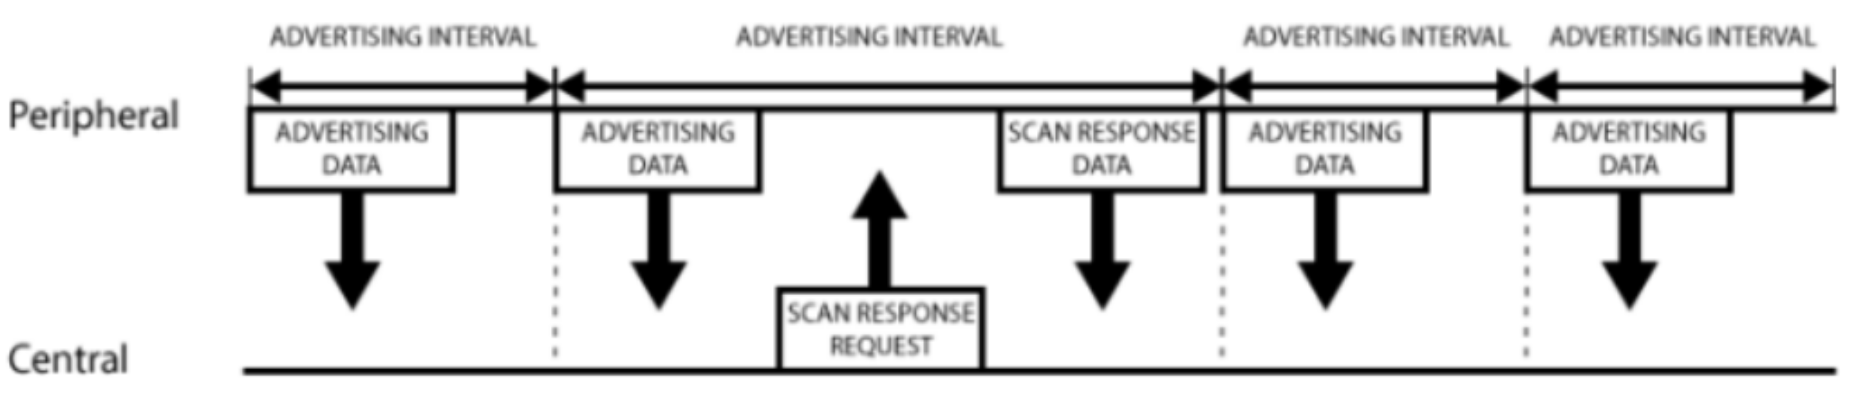
\includegraphics[scale=0.4]{figuras/rn4020/advertising.png}
	\caption{Proceso de anuncio de un dispositivo.}
	\label{advertising}
\end{figure}

Un dispositivo periférico puede definir el intervalo de anuncio, y en cada tiempo en que se alcance este intervalo de anuncio, se enviará un paquete de datos llamado Advertising data. A intervalos largos de anuncios, el dispositivo reduce considerablemente el consumo, pero el equipo es menos sensible a las respuestas si el intervalo de anuncio es de 2 segundos en lugar de 20ms. Si algunos de los dispositivos que se encuentran escuchando estos mensajes de anuncio por parte del periférico está interesado en recibir los datos que agrega el mensaje Scan Payload (y a su vez está disponible en el dispositivo periférico), entonces es posible enviar un mensaje que indica que se requiere el Scan Payload del dispositivo, a lo cual este le responderá con los datos solicitados.

-Transacciones GATT: Un concepto importante para entender GATT es la relación servidor / cliente. El periférico se conoce como el servidor GATT, ya que contiene los datos de búsqueda ATT y las definiciones de servicio y características, y el cliente GATT (el teléfono / tableta), que envía solicitudes a este servidor. 

Al establecer una conexión, el periférico sugerirá un "Intervalo de conexión" al dispositivo central, y el dispositivo central intentará volver a conectar en cada intervalo de conexión para ver si hay nuevos datos disponibles. Es importante tener en cuenta que este "Intervalo de conexión" es sólo una sugerencia, puesto que es posible que el dispositivo central no pueda cumplir con la solicitud porque está ocupado hablando con otro periférico o los recursos del sistema necesarios no están disponibles.

El siguiente diagrama ilustra el proceso de intercambio de datos entre un periférico (el servidor GATT) y un dispositivo central (el cliente GATT), con el dispositivo maestro iniciando cada transacción GATT.\newline

\begin{figure}[H]
	\centering
	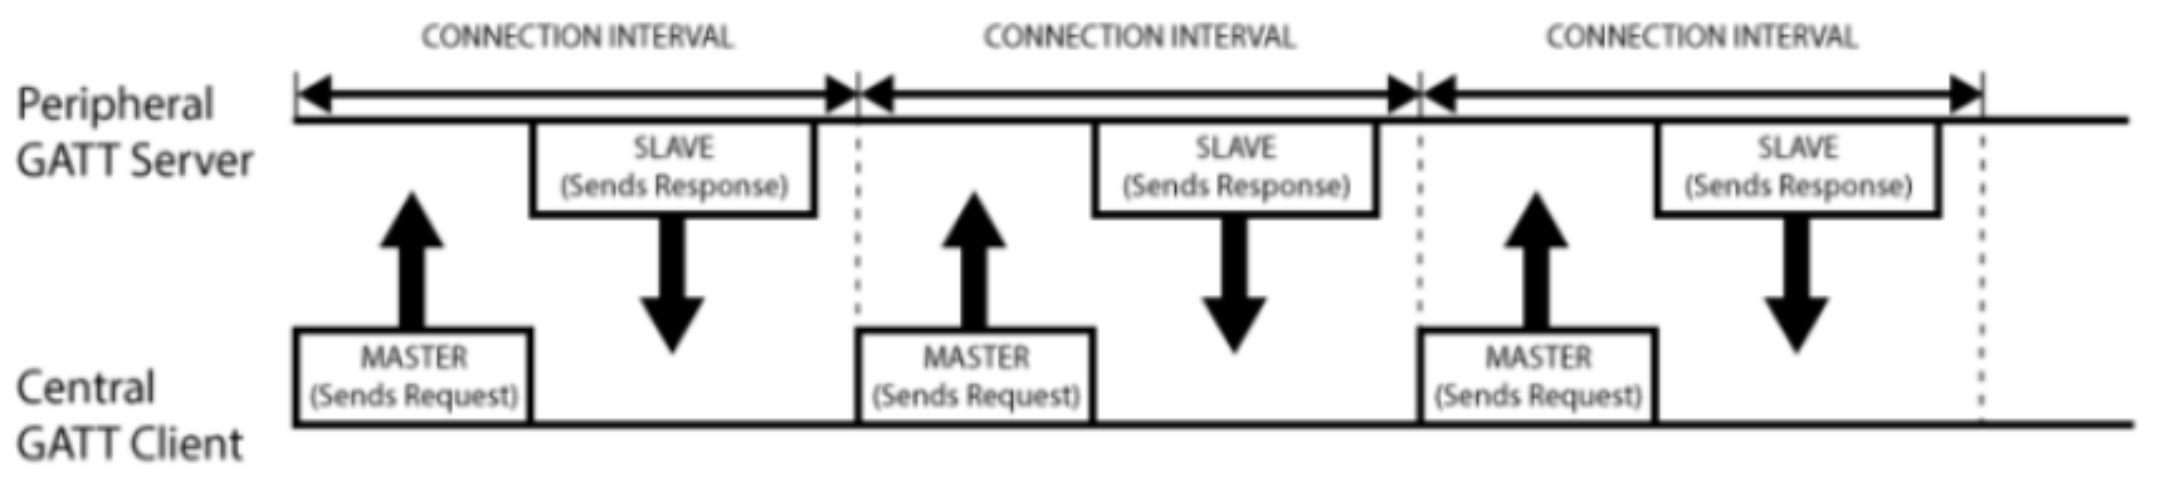
\includegraphics[scale=0.4]{figuras/rn4020/gatt.png}
	\caption{Transacciones GATT.}
	\label{gatt}
\end{figure}



-Perfiles, Servicios, Características y Descriptores: Las transacciones GATT en los dispositivos BLE están basadas en objetos anidados de alto nivel que se denominan Perfiles, Servicios y Características. El orden de estos elementos se muestra a continuación.

\begin{figure}[H]
	\centering
	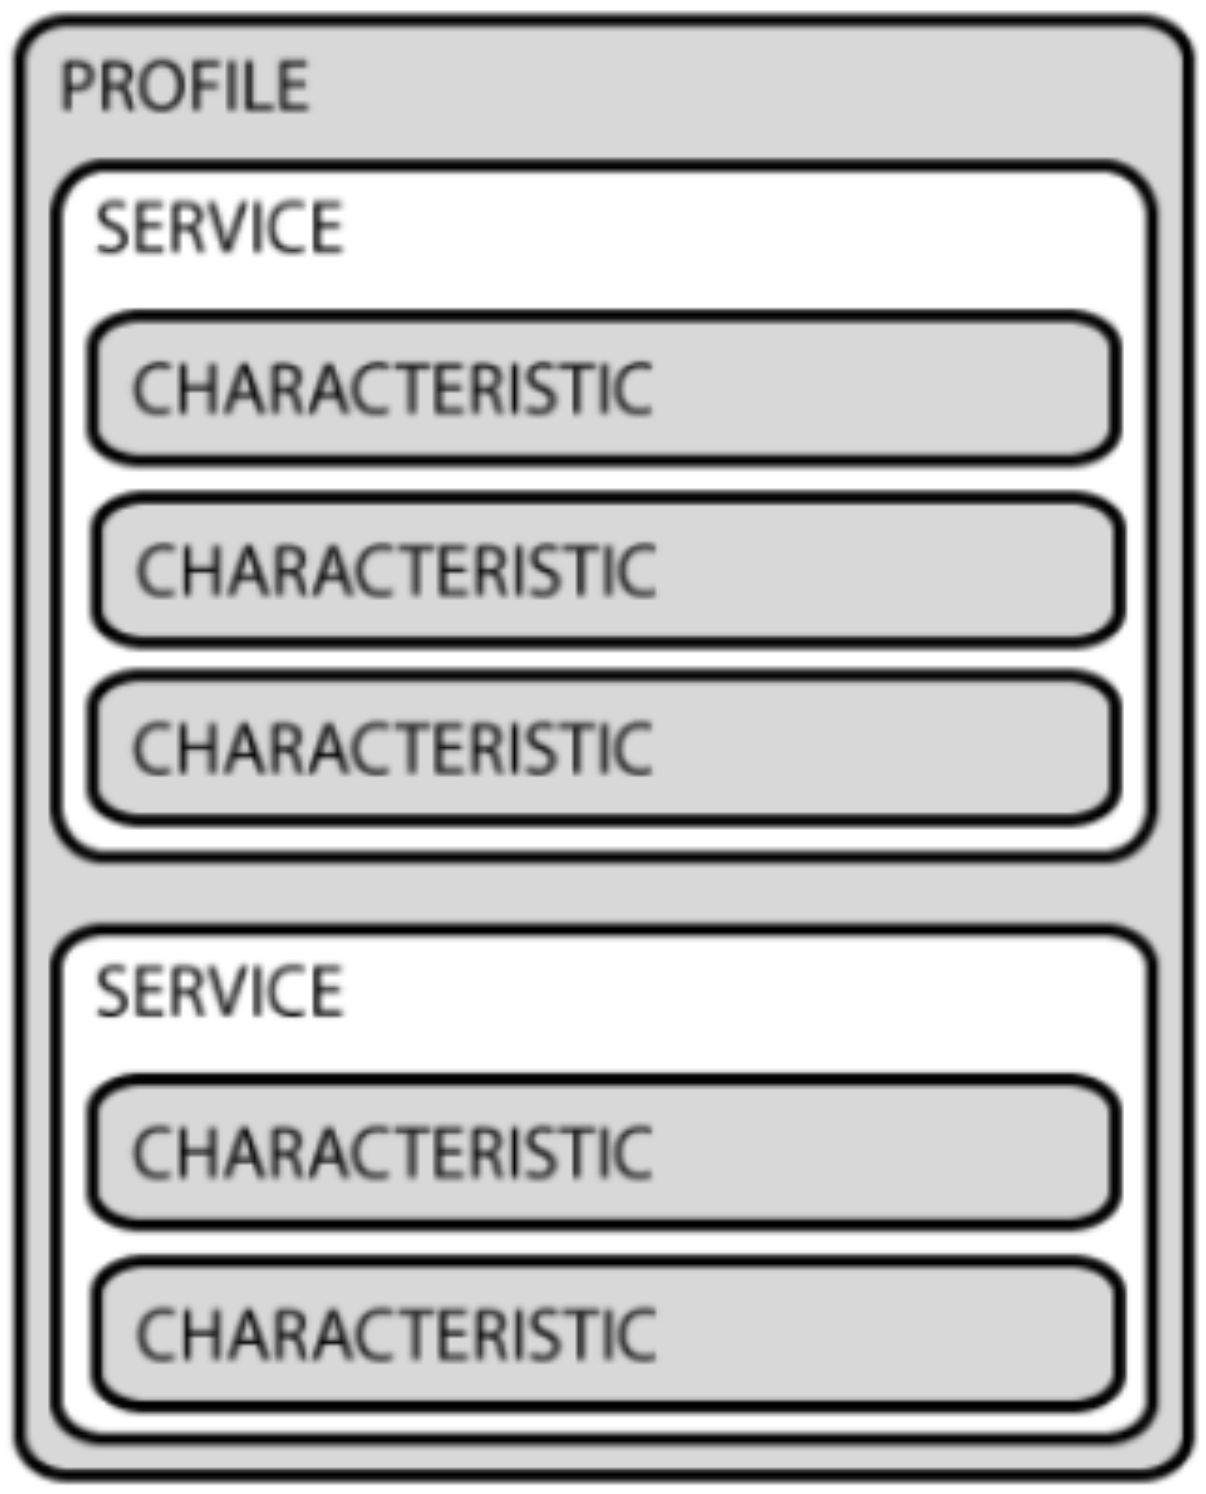
\includegraphics[scale=0.4]{figuras/rn4020/orden_gatt.png}
	\caption{Orden de objetos en transacciones GATT.}
	\label{orden_gatt}
\end{figure}

Un perfil no existe en el propio periférico BLE, sino que es una colección predefinida de servicios que ha sido compilada por el SIG de Bluetooth o por los diseñadores periféricos. El perfil de frecuencia cardiaca, por ejemplo, combina el servicio de frecuencia cardiaca y el servicio de información de dispositivos.\newpage
Los servicios se utilizan para dividir datos en entidades lógicas y contienen porciones específicas de datos llamados Características. Un servicio puede tener una o más características y cada servicio se distingue de otros servicios por medio de un ID numérico único denominado UUID, que puede ser de 16 bits (para servicios BLE adoptados oficialmente) o de 128 bits (para servicios personalizados). Una lista completa de los servicios BLE adoptados oficialmente se puede ver en la página Servicios del Portal de Desarrolladores de Bluetooth.\newline \newline
El concepto de nivel más bajo en las transacciones GATT son las características, que encapsula un único punto de datos (aunque puede contener una matriz de datos relacionados, como valores X / Y / Z de un acelerómetro de 3 ejes, etc.). De forma similar a los Servicios, cada Característica se distingue a través de un UUID predefinido de 16 bits o 128 bits. También se utilizan para enviar datos al periférico BLE, ya que también se puede escribir en la característica. Se puede implementar una interfaz UART simple con un 'Servicio UART' personalizado y dos características, una para el canal TX y otra para el canal RX, donde una característica puede configurarse como de sólo lectura y la otra tiene privilegios de escritura.
Una Característica contiene un único valor y entre 0 y n descriptores que describen el valor de la característica, vale decir, algún rango aceptable o la unidad en caso de ser un valor cuantitativo, hasta una breve descripción de texto. \newpage

-Topología de red a utilizar: Un periférico sólo puede conectarse a un solo dispositivo central (Como un teléfono móvil) a la vez, pero un dispositivo central puede conectarse a varios periféricos. Una vez ya se estableció la conexión entre un dispositivo periférico y un central, la comunicación puede ser bidireccional. Para los fines del proyecto se espera solo una conexión 1 a 1, pero se destaca la comunicación bidireccional posible con este estándar.

\begin{figure}[H]
	\centering
	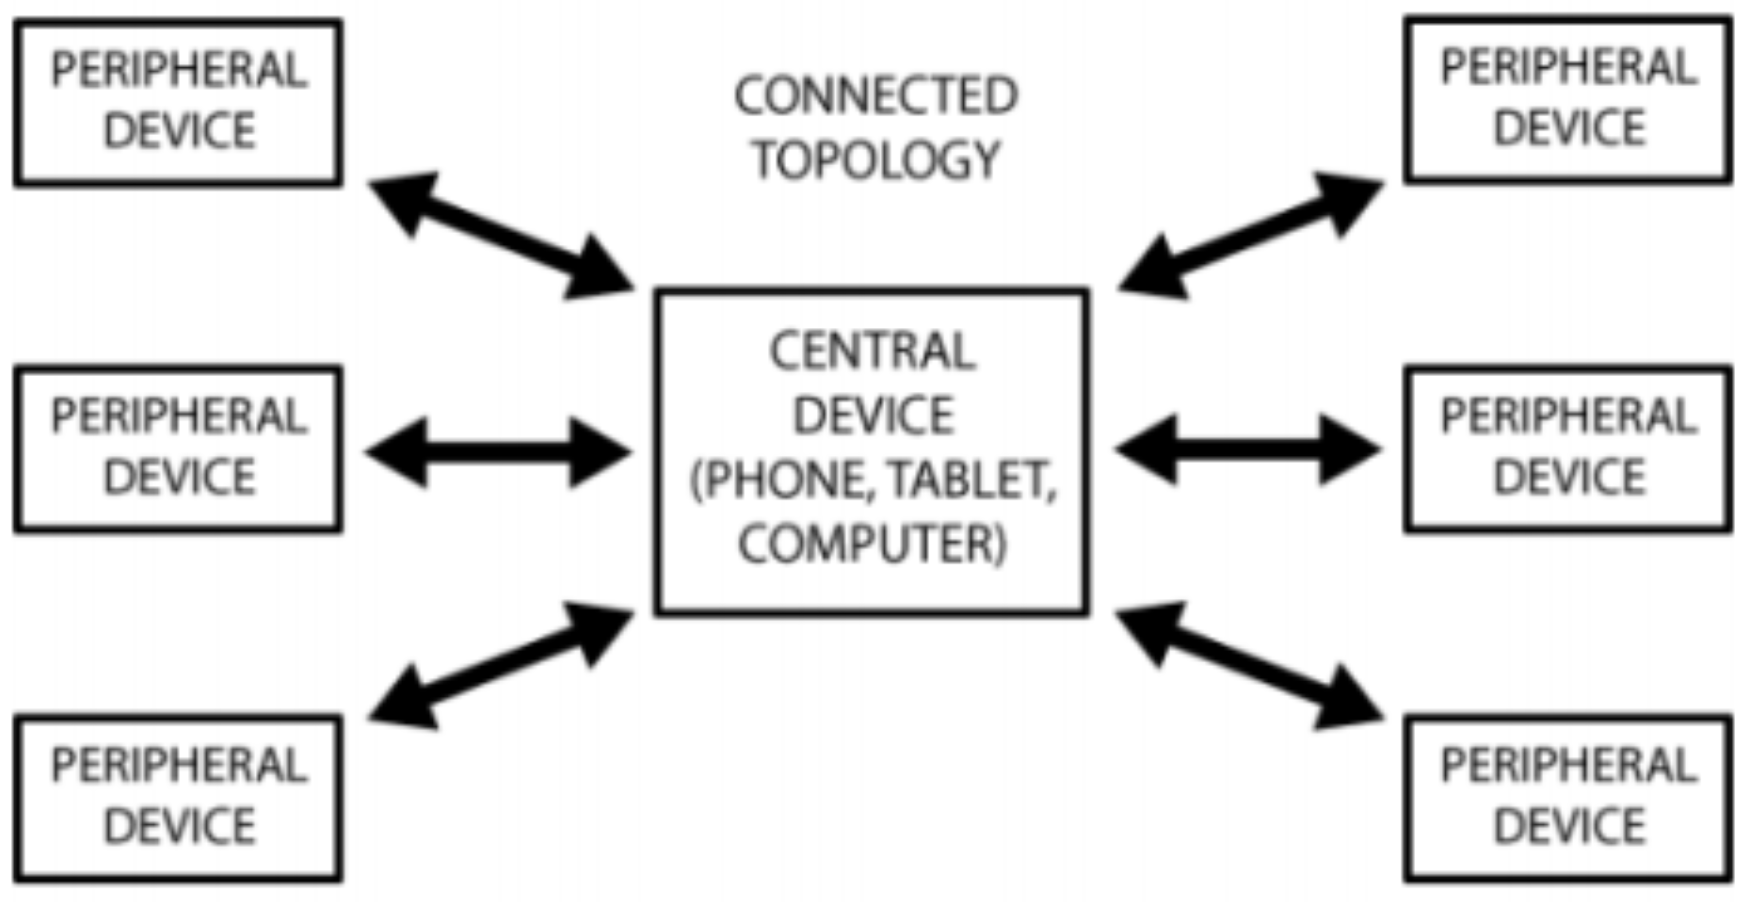
\includegraphics[scale=0.4]{figuras/rn4020/topologia.png}
	\caption{ Topología de red de dispositivos conectados.}
	\label{topologia}
\end{figure}

Algo importante además de todo lo ya mencionado son los distintos estados en los que se pueden encontrar los distintos dispositivos Bluetooth, los cuales varían dependiendo de las versiones Bluetooth y los dispositivos mismos. A grandes rasgos se pueden distinguir 3:

\textbf{Emparejado}: Reconocimiento inicial, en donde se realiza un intercambio de llaves criptográficas (validación por medio de pin) para una comunicación cifrada inmediata.

\textbf{Enlazado/ligado}: Intercambio y almacenamiento de llaves criptográficas (validación por medio de pin), no necesariamente requiere una conexión inmediata, puede realizarse para posteriormente conectar los dispositivos.

\textbf{Conectado}: A partir de algún estado ya mencionado, se continúa con la conexión misma, con la que se espera intercambiar la información objetivo.
\newpage

\section{Características disponibles y selección, autoconexión Bluetooth (desde Android)}

Para definir la comunicación Bluetooth con el chip RN4020 (con perfiles GATT) según lo establecido para el proyecto, se hace necesaria la creación de un perfil, servicios y características privadas. Por esto se definen los parámetros a continuación:

Comando: 

	PZ: Limpiar servicios
	
	R,1: Reinicio

	SF,1 y R,1: Restablecer de fábrica

	SR,20402000 y R,1: Características de chip RN4020

	SS,00000001 yR,1: Habilitación de Servicios Privados

	PS,66ecf52ce19f11e48a001681e6b88ec1: Servicio con UUID (random) privada

	PC,UUID,10,01,01 y R,1: Característica asociada a servicio previo

	SUW,UUID,01: Escritura en característica asociada

La mayoría de opciones es utilizada bajo codificación hexadecimal, como lo son tamaños y ciertas características. A partir del o anterior se establecen 2 formas de reconexión: 

	Auto anuncio: El dispositivo BLE al terminar una conexión automáticamente se hace visible.

	Anuncio manual: El dispositivo BLE requiere de una señal para hacerse visible (con la capacidad de recibir otra instrucción para dejar de serlo).

Se decide usar la segunda opción dado que se optimiza el recurso energético y dota de seguridad al dispositivo al no permitir conectarse a cualquiera sin previa interacción directa con el mismo. Además, se utiliza lo aprendido en el capítulo anterior (Servicios en Android para reconexión) para bajo la documentación del chip RN4020 comunicar (bajo notificaciones que no requieren peticiones del cliente Android) el dispositivo BLE con la aplicación. Cabe destacar que la reconexión se puede hacer automática al especificar la conexión GATT, pero esta demora alrededor de 10 segundos.


%Capítulo 9: Integración de las componentes de la solución
\newpage
% ---------------------------------------------------------------------------------------
\chapter{Integración de las componentes de la solución}\label{mldp}
En esta sección se abordará el hardware utilizado para prototipado y diseño de bluetooth bajo consumo (BLE - bluetooth low energy). 

\section{BLEBee}
Para el prototipado se utilizará un módulo bluetooth BLEBee que ofrece una conexión simple a placas Arduino que posean este puerto. 
BLEBee utiliza un módulo de bluetooth RN4020 el cual ofrece bluetooth versión 4.1.\\
Mediante interfaz UART, este modulo puede ser configurado para actuar como módulo central o periférico cuando establezca una conexión.\\
Para conocer mas el funcionamiento de este módulo primero hay que conocer mejor la conexión XBee.

\begin{figure}[H]
\centering
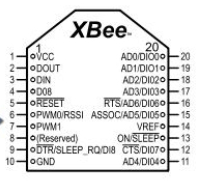
\includegraphics[scale=1]{figuras/bluetooth/xbee.png}
\caption{Forma y Pines de puerto XBee}
\label{xbee}
\end{figure}

Como se puede observar en la figura \ref{xbee} el puerto XBee ofrece una conexión de 20 pines con usos generales que se utilizan por distintos dispositivos, en este caso bluetooth.\\
En el caso de BLEBee la distribución de los pines se puede observar en la figura \ref{blebee}

\begin{figure}[H]
\centering
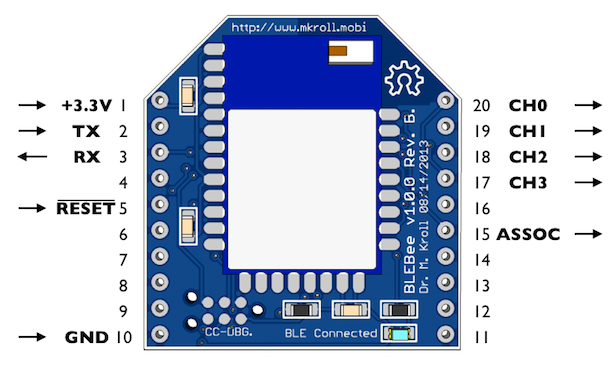
\includegraphics[scale=0.5]{figuras/bluetooth/blebee.png}
\caption{Distribución de pines BLEBee}
\label{blebee}
\end{figure}

Comparando la figura \ref{xbee} con la figura \ref{blebee} se puede observar los pines mas relevantes a la hora de diseñar un módulo bluetooth en el dispositivo, siendo los pines mas importantes, y contrastando con el datasheet, los que se muestran en la tabla \ref{pines}

\begin{table}[H]
\centering
\begin{tabular}{| c | c | c |}
\hline
\multicolumn{1}{|c|}{\textbf{Nº Pin}}&
\multicolumn{1}{c|}{\textbf{Nombre}}&
\multicolumn{1}{|c|}{\textbf{Descripción}}\\ \hline
5  & UART TX & Transmisor UART\\ \hline
6  & UART RX & Receptor UART\\ \hline
7  & WAKE\_ SW & Despertador de modo deep sleep\\ \hline
10 & Led Conexión  & Led indicador de conexión\\ \hline
12 & Led Actividad & Led indicador de actividad\\ \hline
\end{tabular}
\caption{Pines relevantes módulo RN4020}
\label{pines}
\end{table}

\newpage
\section{Comunicación UART}

La comunicación UART (Universal Asynchronous Receiver-Transmitter) es un formato de comunicación serial donde el formato y la velocidad de transmisión son configurables. Un UART puede ser un circuito integrado independiente pero en la actualidad vienen incluidos en los microcontroladores.\\
Para entender mejor como funciona la comunicación serial mediante UART hay que observar la figura \ref{UART}

\begin{figure}[H]
\centering
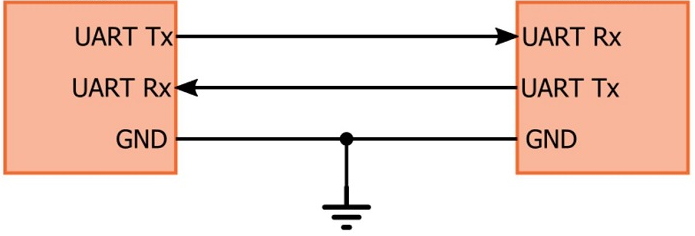
\includegraphics[scale=0.8]{figuras/bluetooth/uart.png}
\caption{Configuración para comunicación UART}
\label{UART}
\end{figure}

La comunicación UART cuenta de 2 pines TX (transmisor) y RX (receptor) el cual se conecta al Receptor y transmisor del microcontrolador respectivamente.

\section{Diseño del módulo bluetooth}
Finalmente contrastando lo visto anteriormente y con referente a la tabla \ref{pines} se puede diseñar el esquemático del integrado.\\
Pin 5 y 6 corresponden a la comunicación UART como se explica en la figura \ref{UART}. Es necesario conectar los pines 10 y 12 con diodos led ya que son pines indicadores, el pin 10 indica el estado de la conexión con un led verde y también se recomienda conectar un led azul al pin 12 para ver el estado de actividad (ej. Si se está enviando información o está dormido).\\
El pin 7 cumple la función de despertar el módulo bluetooth cuando se encuentre dormido emitiendo desde el microcontrolador una señal de $3.3[V]$.\\
\begin{figure}[H]
\centering
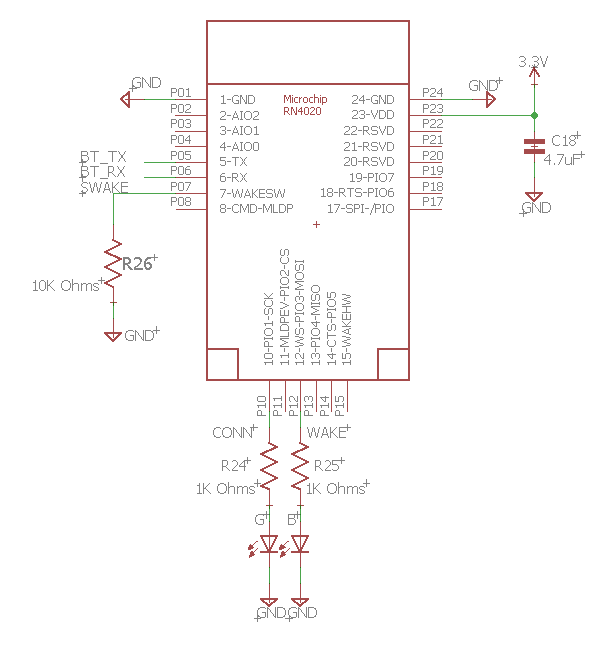
\includegraphics[scale=0.8]{figuras/bluetooth/eagle.png}
\caption{Esquemático bluetooth diseñado en EagleCAD}
\label{eagle}
\end{figure}

Como se puede observar en la figura \ref{eagle} se conecta el módulo bluetooth con los pines descritos. Se utiliza un condensador en la alimentación de módulo para regular el voltaje de la entrada.






%Capítulo 10: Prototipo funcional V1
\newpage
% ---------------------------------------------------------------------------------------
\chapter{Prototipo funcional V1}\label{proto1}

Para continuar con el desarrollo del proyecto, se deben hacer funcionar las distintas partes (sensores, microcontrolador, módulo Bluetooth, Smartphone y servidor) como un todo y para ello se crea un primer hito de prototipado con el cual se espera alcanzar esta integración. Además de lo anterior, se espera poder hacer pruebas que asienten o desmientan decisiones de diseño y configuración, siempre con miras a los requerimientos generales del proyecto.

\section{Configuración final RN4020}

En el apartado del microcontrolador junto al módulo Bluetooth, se utiliza un archivo .ino con los parámetros necesarios y un ciclo de ejecución con el cual ofrecer la funcionalidad del envío de datos desde los sensores al Smartphone.

En esta primera configuración se hace uso de un Script para la configuración básica del chip RN4020 por parte del microcontrolador, se establece la visibilidad como activa desde el inicio de operación, se utilizan los parámetros por defecto al mínimo de conexión Bluetooth: Latencia (tiempo de respuesta), intervalo de conexión (frecuencia con que una comunicación es establecida), timeout(tiempo de espera antes de cancelar la comunicación) y se habilita la encriptación en la comunicación Bluetooth (AES-128, cirptografía simétrica).

Respecto a la comunicación entre el microcontrolador y el módulo se observa que los Baudios máximos se encuentran en los 19.200 [S/s], pasando por 2.400 [S/s] y 9.600 [S/s].\newpage


\section{Análisis de rendimiento por codificación }

En esta oportunidad se le da prioridad a la configuración del ECG por sobre los datos de temperatura, pese ya a tener configurada la característica asociada a ambos. Por lo que se realizan distintas pruebas modificando parámetros relevantes como la potencia (de transmisión del chip RN4020), la seguridad, cantidad de datos por envío y Baudios. Cabe mencionar que los datos deben ser convertidos a hexadecimal para ser entregados al módulo Bluetooth, por lo que se deben convertir tanto en el microcontrolador como en la aplicación móvil.

En la figura \ref{benchmark} se utilizaron:

\textbf{Distancia}:  Fija a 1 metro.

\textbf{Potencia}: Variable 4 y 7, a -2.5 [dBm] y 7.5 [dBm] respectivamente.

\textbf{Seguridad}: Enlazado y no enlazado.

\textbf{Línea vista}: No.

\textbf{Datos}: Hexadecimal de 1 [byte] representando enteros entre [0-255].


\begin{figure}[H]
	\centering
	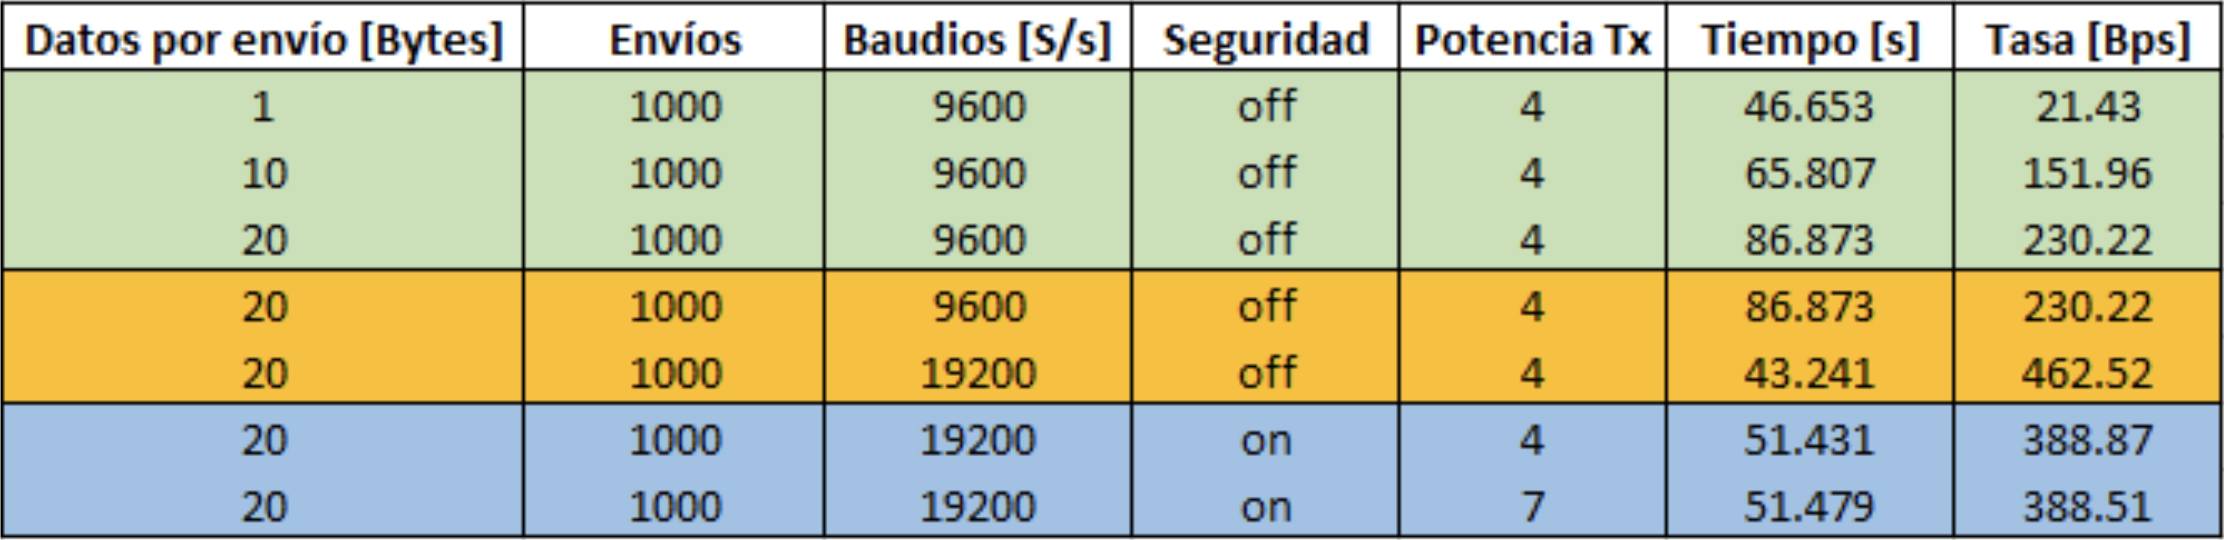
\includegraphics[scale=0.3]{figuras/proto1/benchmark.png}
	\caption{Resultados, pruebas de configuración ECG. Fuente: Elaboración propia}
	\label{benchmark}
\end{figure}

Con lo cual se justifica el uso de paquetes de 20 datos (máximo permitido en una misma instrucción por el módulo RN4020) por envío. Logrando así una frecuencia de al menos 200 [Bps] en el envío de datos si fuere necesario.
Además, se destaca que la seguridad no afecta significativamente y dada la distancia, la potencia de transmisión tampoco. Pese a lo anterior se baraja la posibilidad de usar una resolución de 10 bits (resolución máxima del sensor) a través del uso de 2 bytes hexadecimales, alcanzando un máximo de 10 datos por envío.

\section{Elementos en Android}

Luego de haber obtenido la base de aplicación en función del ejemplo en la página oficial de Microchip, la cual entrega las herramientas para comnunciarse con el chip RN4020, se busca dar forma a una aplicación que cumpla con las características del proyecto y que por el momento sea funcional en torno a lo obtenido hasta el momento.

Android es un SO ampliamente utilizado y por ende posee una gran comunidad a sus espaldas, las cuales frecuentemente otorgan librerías y mejoras constantes además de su propio responsable (Google). Con lo anterior en mente, se hace la búsqueda de distintas herramientas capaces de ofrecer funcionalidad y flexibilidad al proyecto, las cuales se describirán brevemente en conjunto con una explicación de por qué su uso frente a otras alternativas (no necesariamente mencionadas). Cabe destacar que el presente documento se hace al año 2018 y por ende con las capacidades actuales presentes en el desarrollo de una aplicación Android.\newline

\begin{figure}[H]
	\centering
	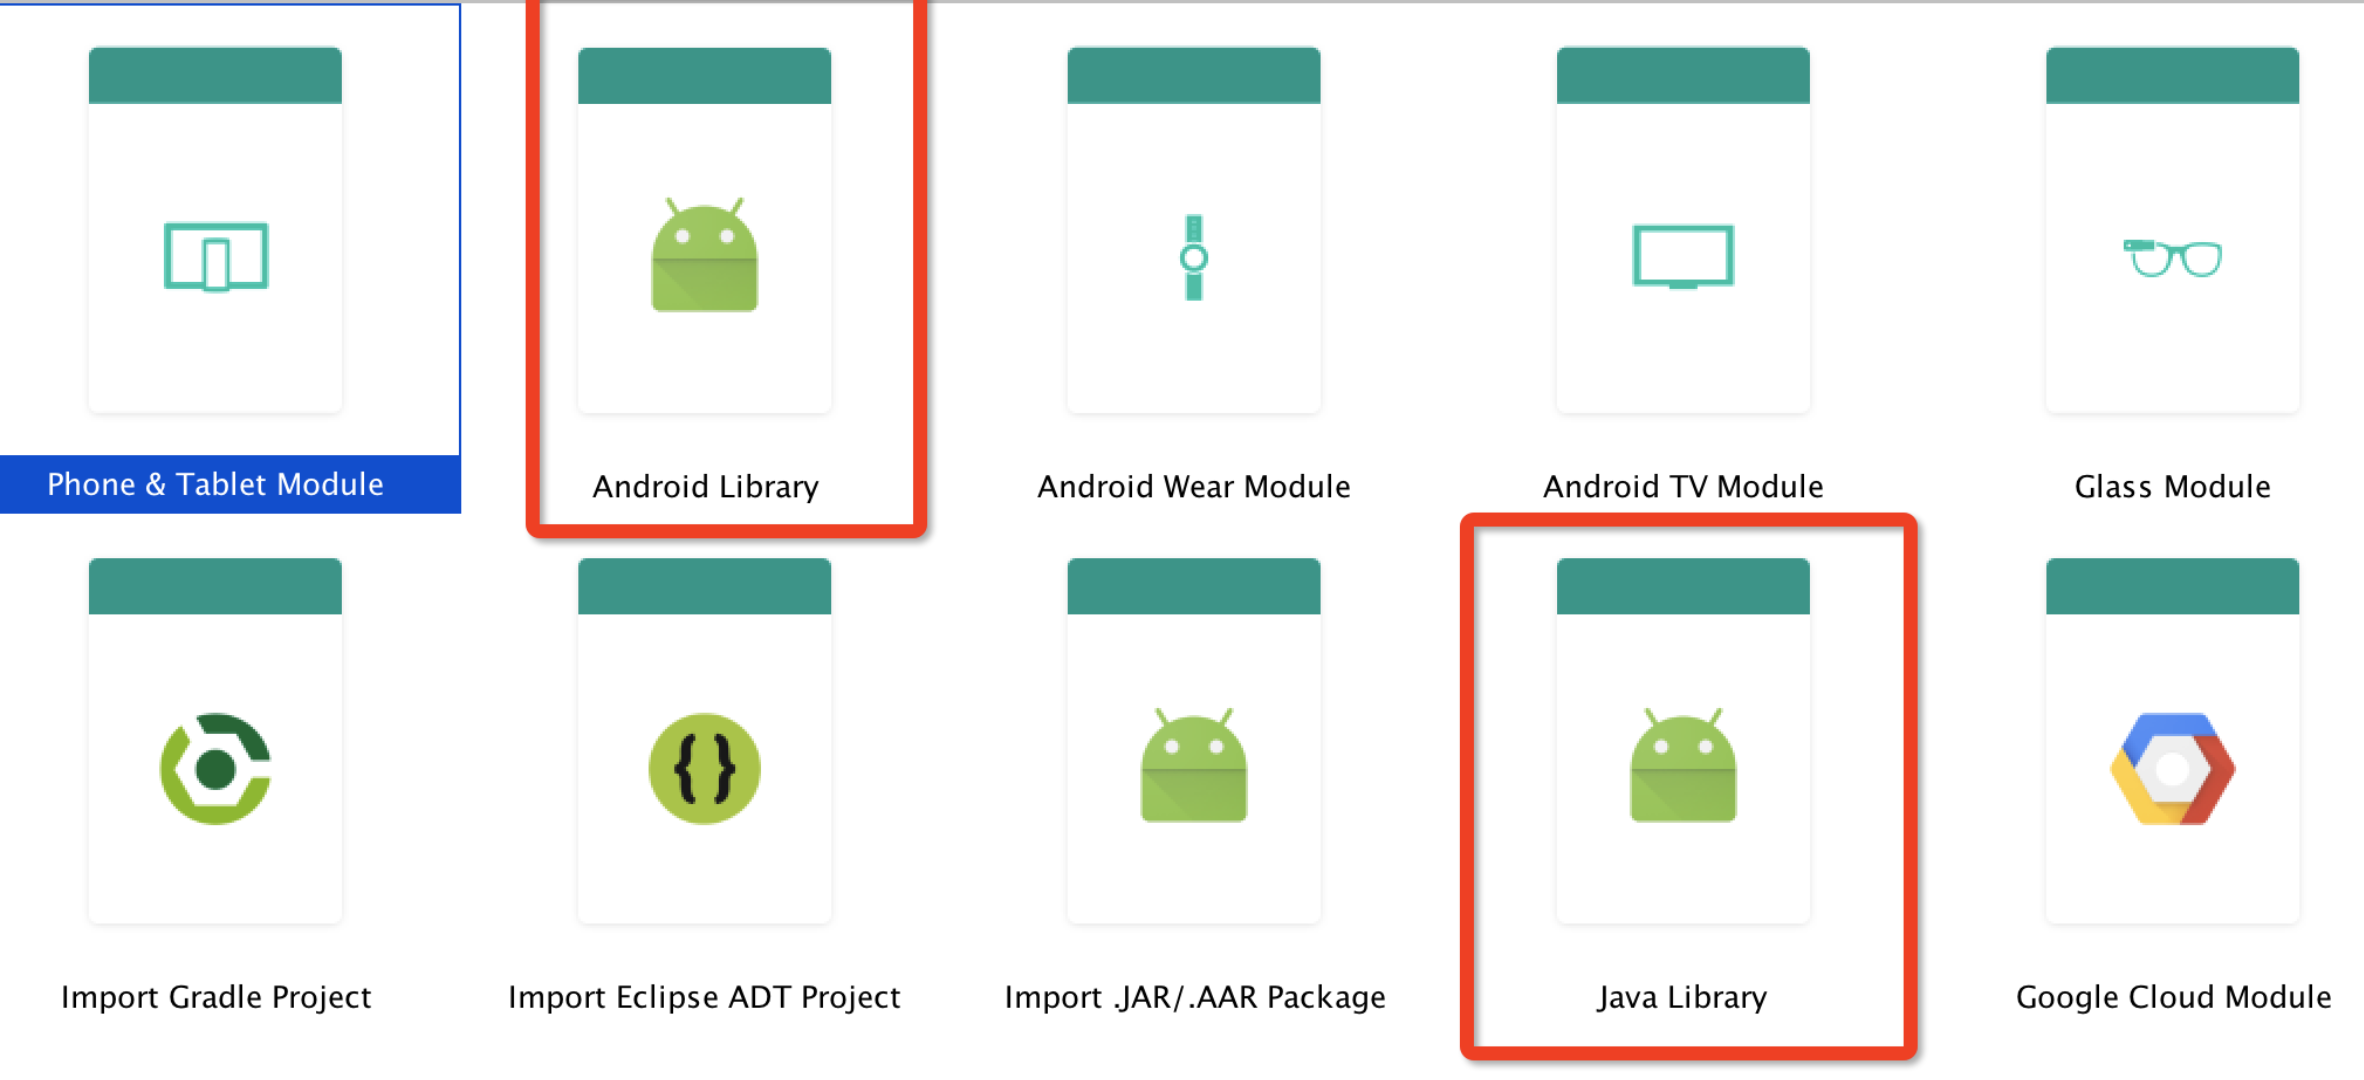
\includegraphics[scale=0.3]{figuras/proto1/library.png}
	\caption{Uso de librerías en Android. Fuente: Android Studio}
	\label{library}
\end{figure}

 \newpage

\subsection{RecyclerView}

En Android, existen diversas formas de generar visualmente listas para los usuarios, pero actualmente gracias a Google se cuenta con algo llamado RecyclerView. La cual funciona como contenedor de una lista como cualquier otra, pero pensada en el alto rendimiento (gran cantidad de elementos) y una estética cuidada en la fluidez de la misma. 

Para una aplicación como la presente no se hace necesario el uso de esta librería, dado que no se tiene una gran cantidad de elementos que desplegar en pantalla, pero siempre es bienvenida la velocidad de codificación que proporciona al presentar una arquitectura de plantillas sobre las cuales generar elementos. Así, es utilizada en el proyecto actual para contener distintos tipos de conexión  con su respectivo estado: Al servidor, con el módulo Bluetooth, y con el servicio propio de la aplicación.\newline

\begin{figure}[H]
	\centering
	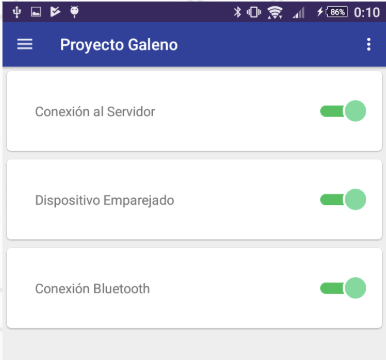
\includegraphics[scale=1]{figuras/proto1/recycler.png}
	\caption{Uso de RecyclerView. Fuente: Elaboración propia}
	\label{recycler}
\end{figure} 

\newpage

\subsection{Códigos QR}

Dado que el proyecto utiliza un emparejamiento con un dispositivo Bluetooth, es importante recordar que para lograr esto existen distintas técnicas, entre las que destacan el escaneo (alto consumo de potencia, lento y engorroso si existen diversos dispositivos), ingreso manual de la dirección física MAC del dispositivo al cual conectarse (lento y engorroso) y por ingreso automático (utilizando la cámara como medio físico y alguna codificación ya establecida). Es en este último punto en donde los códigos de barra surgen como una opción rápida y cómoda, más aún cuando se utiliza a los códigos QR, los cuales estandarizan la codificación básica de cualquier cadena de texto. Otorgando así comúnmente direcciones URL, de las cuales se obtienen diversos recursos (imágenes, video, texto, entre otros).

Es por lo anterior que se decide emplear a los códigos QR como la forma más efectiva de entregar la dirección física de los módulos Bluetooth, con la cual la aplicación podrá efectuar el emparejamiento respectivo.

Para esta acción existen diversas librerísa disponibles, pero de entre ellas se destaca a ZXING, la cual ofrece tanto la creación como la lectura de distintos tipos de códigos. Hace unos años esta librería solo podía usarse en conjunto con una aplicación, pero actualmente es posible encontrarla por separado: QRCodeReaderView es una versión modificada de ZXING que permite leer códigos QR de forma simple y rápida (aunque con pocas opciones de personalización de interfaz).

\begin{figure}[H]
	\centering
	
\includegraphics[scale=0.6]{figuras/proto1/qr.png}
	\caption{QR con MAC de dispositivo Bluetooth. Fuente: Elaboración propia}
	\label{qr}
\end{figure}

\subsection{Fragment}

Este es un elemento básico en Android y es utilizado como una versión menor de las Activitys, es utilizado comúnmente como contenedor de vistas menores y controlados en conjunto por una Activity.
Su uso en el proyecto fue decidido por el menú lateral escogido para albergar las distintas vistas de la aplicación.

\begin{figure}[H]
	\centering
	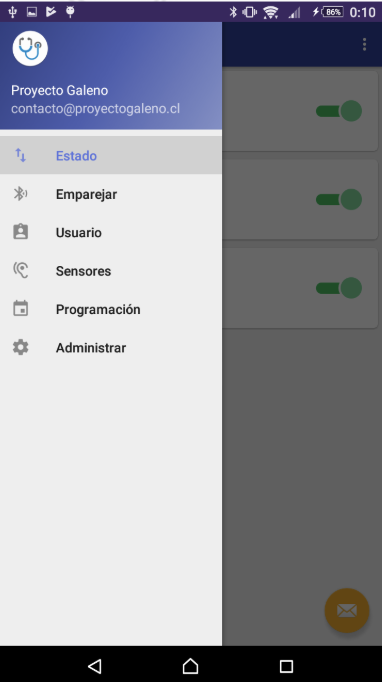
\includegraphics[scale=1]{figuras/proto1/fragment.png}
	\caption{Menú lateral comprendido por distintos Fragment. Fuente: Elaboración propia}
	\label{fragment}
\end{figure}

Si bien no todas esas vistas fueron implementadas (Usuario y Programación) en este punto, se tuvo claridad de las mismas desde un inicio y se tuvo consideración en la facilidad de uso, agrupando las opciones según función.

\subsection{MPAndroidChart}

La visualización es una funcionalidad necesaria con el fin de validar pruebas y otorgar al mismo tiempo un prototipo con mayor solidez hacia la contraparte. Es por esta razón que se analizaron distintas opciones de librerías, dentro de las cuales destacó MPAndroidChart, librería nativa de Android, con gran rendimiento y opciones de personalización. Es sencilla de utilizar y ofrece la posibilidad de gráficos en tiempo real, dependiendo del dispositivo se pudieron obtener sobre 1000 puntos al mismo tiempo con gran fluidez, algo realmente importante si se considera que el ECG posee un gran flujo de datos (típicamente de 50 [Hz] - 150 [Hz]).

\begin{figure}[H]
	\centering
	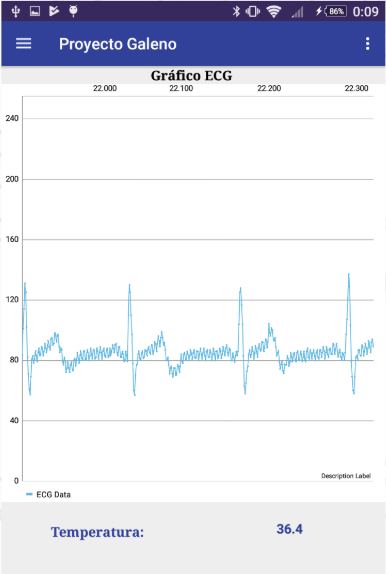
\includegraphics[scale=1]{figuras/proto1/graph.png}
	\caption{Gráfico en tiempo real con datos de ECG por Bluetooth. Fuente: Elaboración propia}
	\label{graph}
\end{figure}

Como se puede observar en la figura \ref{graph}, se observa gran cantidad de ruido, aspecto corregido hasta cierto punto en posteriores iteraciones.

\subsection{Shared Preference}

El proyecto requiere que la dirección MAC sea almacenada en alguna memoria persistente con el fin de poder reconectar los dispositivos de ser necesario: Al apagar el Smartphone o el Arduino, al aumentar demasiado la distancia, entre otros. La dirección MAC no es otra cosa que una cadena de texto, por lo que un almacenamiento básico es suficiente para los objetivos del proyecto.

Por lo anterior se decanta por la utilización de Shared Preference (Preferencias compartidas) como el método de almacenamiento, esta es una característica que ofrece Android de forma base, la cual permite por aplicación un almacenamiento tipo llave-valor, estilo diccionario. La cual es accesible solo desde la misma aplicación o compartida entre distintas aplicaciones, pero con persistencia al cierre de las mismas (lo que realmente es fundamental para el proyecto).

\subsection{Inicio automático de Servicio y otros}

En esta sección se detallará un poco más sobre los elementos del menú y el  comportamiento del primer prototipo del proyecto:

\textbf{Estado}: RecyclerView con distinto estados de conexión (Servidor, BT y Servicio).

\textbf{Emparejar}: Lector de códigos QR para asociar MAC de un dispositivo.

\textbf{Sensores}: Presentación visual de los datos recibidos en tiempo real.

\textbf{Usuario}: Datos almacenados en Android del paciente (aún sin implementar).

\textbf{Programación}: Futura mejora para mostrar próximas tomas de datos.

\textbf{Administración}: Manejo del estado del servicio principal.

Respecto a su comportamiento, se establece por medio del Manifest (archivo de cada proyecto en Android que controla permisos, articula las distintas Activity y ciertos parámetros generales) la apertura del servicio al arranaque del SO, mientras el servicio se encuentre activo se encarga de mantener encendido el adaptador Bluetooth del Smartphone y se utiliza la opción de enlazado provisto por el SO Android (por fuera de la aplicación y mencionado al final del capítulo 8).
 



%Capítulo 11: Prototipo funcional V2
\newpage
\chapter{Prototipo funcional V2}\label{proto2}

Luego de un primer prototipo, se analiza el funcionamiento general para planificar cambios y mejoras necesarias. Entre las que destacan un control sobre el envío de datos desde los sensores y una optimización de código en Arduino (relevante por la baja frecuencia de operación que posee frente a las exigencias del proyecto).

Los detalles se presentan a continuación, aunque adelantando que los cambios principales de esta nueva versión fueron realizados a la programación del microcontrolador y su sincronización con la aplicación.

\section{Control de sensores por Android}

Un aspecto fundamental para el proyecto es la posibilidad de controlar el inicio y el fin de las mediciones desde la aplicación, permitiendo en una iteración posterior su control desde la web.

Para este efecto, se desarrolla un protocolo de comunicación con el cual se espera sincronizar las acciones entre los dos principales entes (microcontrolador con módulo Bluetooth y aplicación Android).

Se comienza estableciendo un conjunto de instrucciones homogéneas con las cuales los dispositivos puedan ejecutar órdenes:

\textbf{00}: Detener medición

\textbf{10}: Iniciar solo medición de ECG

\textbf{01}: Iniciar solo medición de T

\textbf{11}: Iniciar ambas mediciones \newpage

Como se puede observar, se utiliza un sistema binario en el cual con 2 bit se logran controlar 4 estados fundamentales. Se escoge esta arquitectura dada su fácil escalabilidad y sencilla comprensión al asignar 0 o 1 a cierta posición asociada (y preacordada) a algún sensor.

Esto en conjunto con un Handler (ejecución de una tarea en otro hilo) en Android, permite el control temporal de estas instrucciones. Logrando así que al momento que la aplicación recibe una petición de medicón, ésta sea comandada por el Handler que a su vez tiene un Timer asociado, con el cual se podrá controlar la ejecución de la medición por una cantidad de tiempo preestablecida.

\begin{figure}[H]
	\centering
	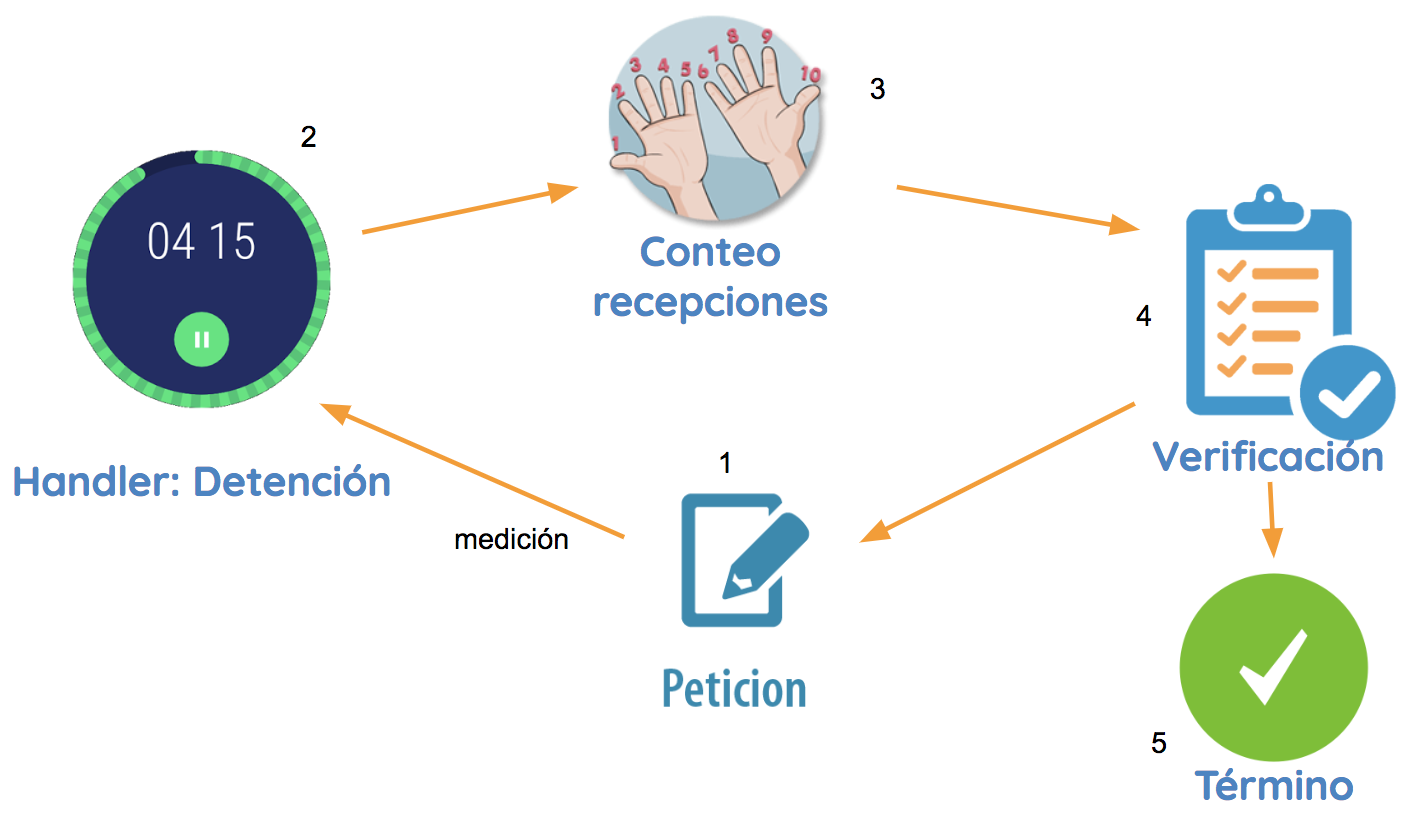
\includegraphics[scale=0.5]{figuras/proto2/handler.png}
	\caption{Control de peticiones por Handler y repetición}
	\label{handler}
\end{figure}

En la figura \ref{handler} se pueden observar los distintos estados asociados a una medición: Petición, medición, detención, conteo, verificación y término.

Al acabar con la medición, el microcontrolador comunica la cantidad de paquetes enviados asociados a cada sensor, cantidad que es verificada con los recibidos en la aplicación y dependiendo de esto último se repite la petición de forma automática o se da por terminada la medición. \newpage

Las secuencias de control corresponden a una cadena de caracteres compuesto por AA y FF al inicio y término respectivamente de una medición, seguidos por 4 caracteres contenedores de 2 byte hexadecimales con el número de paquetes enviados (0 a 65536 paquetes).

Esto último supone una restricción en la cantidad máxima de paquetes enviados por medición:

\textbf{ECG}: Con una tasa de 150 [Hz] | Máximo 6.8 minutos por medición.

\textbf{T}: Con una tasa de 1 [Hz] | Máximo 18.2 horas por medición.

\section{Renovación de servidor Arduino}

Considerando la opción de microcontrolador escogido (Arduino UNO), se tiene una limitante importante en cuanto a la potencia de procesamiento presente, la cual se limita a la frecuencia de operación con la que cuenta el chip ATmega328 que es de 16 [MHz]. 

Por esta razón se hace indispensable una programación prolija y con miras en la optimización en la ejecución de instrucciones. En este sentido, se realizan diversos cambios al código fuente del microcontrolador (se pueden ver con detalle en los Anexos):

Control del ciclo principal de operación bajo milisegundos a microsegundos.

Uso de punteros en vez de copia de memoria para el manejo de arreglos de char.

Uso de condiciones según precedencia y uso de else if según casos más frecuentes.

Control de estados por variables, minimizando verificaciones innecesarias.

\newpage

\section{Análisis de resolución y frecuencia para ECG}

Pasando directamente al manejo del ECG por parte del controlador, se realizan pruebas para establecer frecuencias necesarias y verificar nivel de resolución mínimas, entre las que se destacan los siguientes resultados.

\begin{figure}[H]
	\centering
	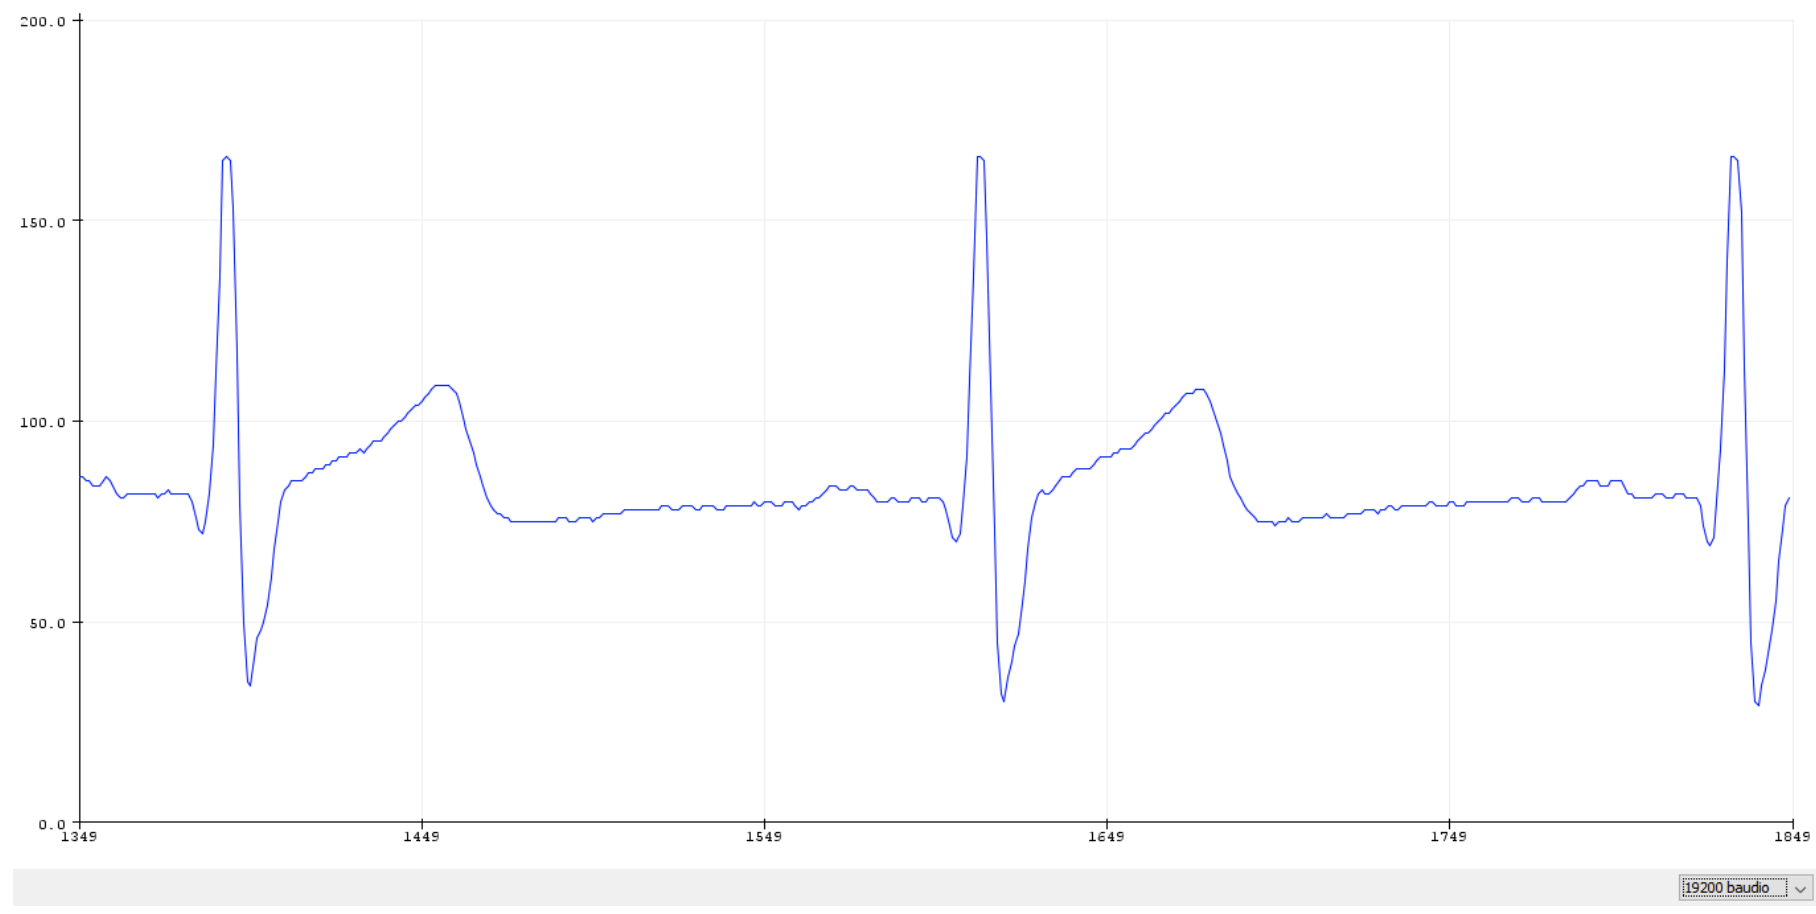
\includegraphics[scale=0.4]{figuras/proto2/8bit.png}
	\caption{ECG a 300 [Hz] y 8 bit de resolución}
	\label{8bit}
\end{figure}

\begin{figure}[H]
	\centering
	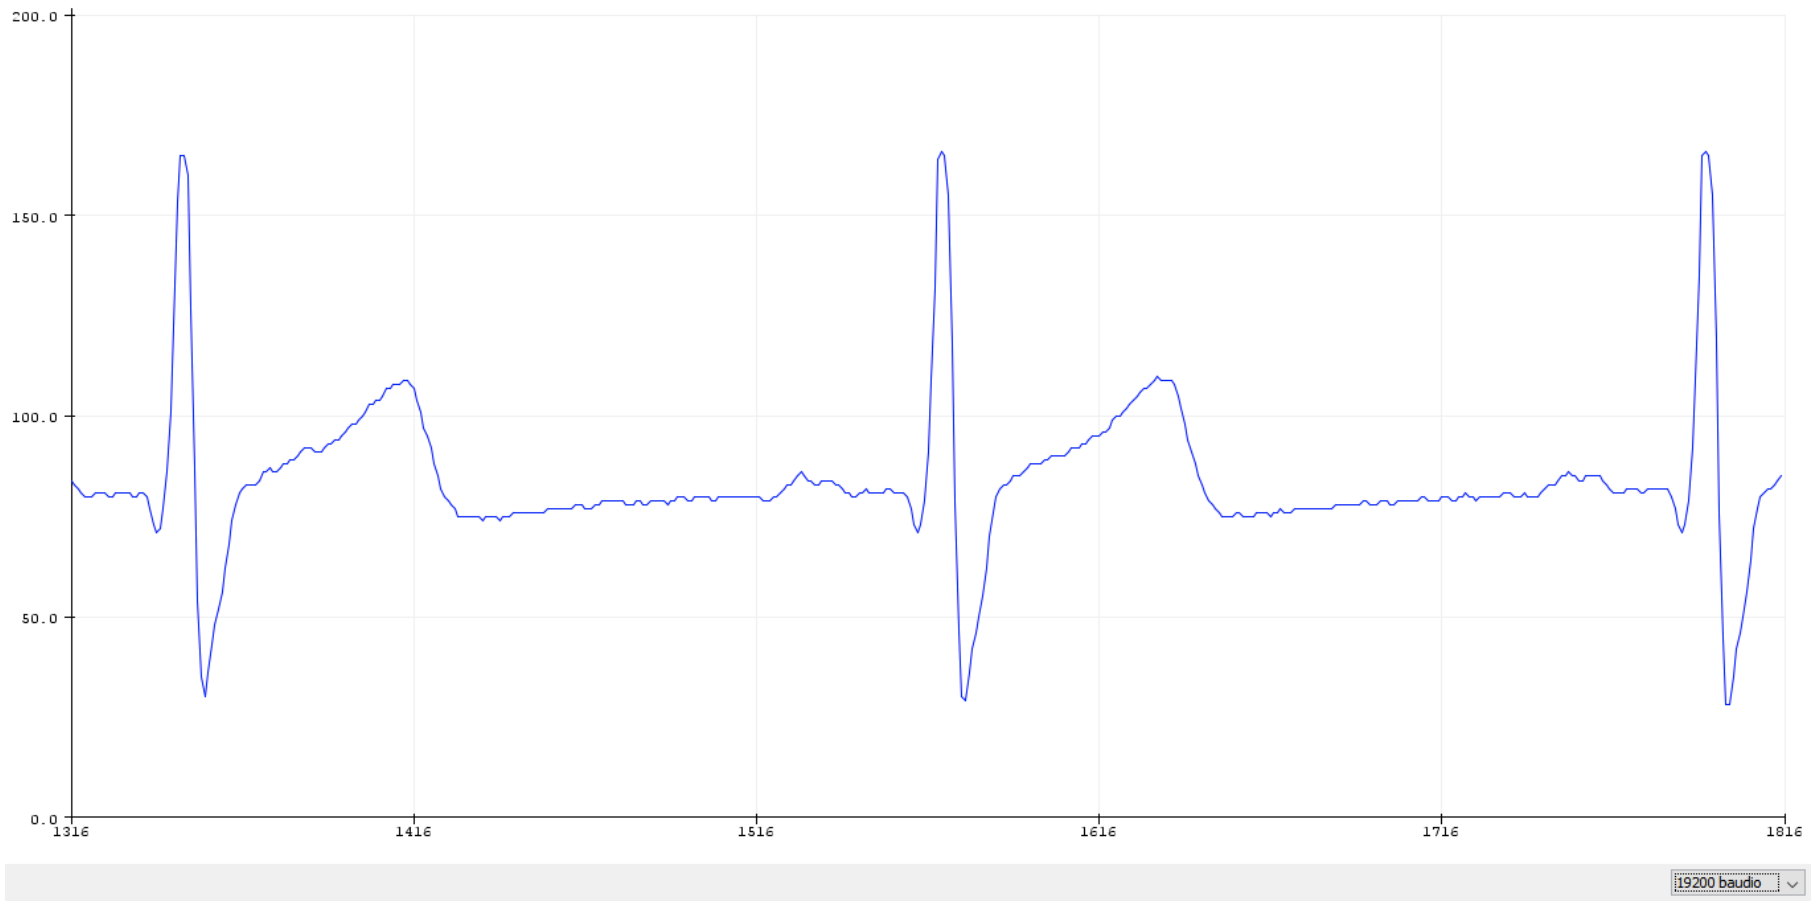
\includegraphics[scale=0.4]{figuras/proto2/10bit.png}
	\caption{ECG a 300 [Hz] y 10 bit de resolución}
	\label{10bit}
\end{figure}

\newpage

Como se puede obervar en las figuras anteriores, la resolución obtenida utilizando 8 bit o 10 bit no representa un cambio significativo a nivel visual, mientras que a nivel de procesamiento y almacenamiento sí posee gran injerencia (valor máximo: 256 y 1024 respectivamente). 

Esto es especialmente importante cuando se tiene en cuenta que la comunicación hexadecimal funciona de forma óptima con información condensada en múltiplos de 8 bit, puesto que la representación de 1 byte (8 bit) es posible por medio de solo 2 caracteres hexadecimales que son exactamente el byte de información.

Así, se decide emplear esta resolución para la captura y comunicación de los datos de ECG, sin miedo a perder información o tener sobrecarga de caracteres, en una comunicación con paquetes contenedores más grandes que la información mínima.

Se hicieron pruebas de frecuencia para el ECG, probando valores entre 50 [Hz] y 1.000 [Hz]. Como resultado de esto se estableció un mínimo de 50 [Hz] de operación, una base esperable de 150 [Hz] y un máximo de 300 [Hz], los anteriores valores por condensación visual de los datos (se observa una compresión horizontal de las gráficas a menores frecuencias y lo contario para frecuencias mayores).

\begin{figure}[H]
	\centering
	\includegraphics[scale=0.4]{figuras/proto2/1000hz.png}
	\caption{ECG a 1.000 [Hz] y 10 bit de resolución}
	\label{1000hz}
\end{figure}

\section{Base de datos local (comparativa Realm, SQLite) }

De nada sirve obtener y comunicar datos si estos no son almacenados y estudiados posteriormente, es por ello que se contempló desde el inicio del proyecto el uso de una base de datos local para la aplicación (útil especialmente para mediciones sin cobertura) y una base de datos propia del servidor web.

En Android existen principalmente dos grandes alternativas respecto a bases de datos: SQLite y Realm (ambas relacionales y con esquema llave-valor). La primera de ellas, SQLite es un motor de base datos ampliamente utilizada y disponible desde los inicios del SO Android, sus grandes ventajas son la gran penetración que ya posee en los desarrolladores y los distintos sabores entenidos en las librerías que lo implementan.

La segunda alternativa es relativamente nueva pero con un potencial enorme, dada su facilidad de uso, gran rendimiento, visualización de datos con aplicaciones externas, disponibilidad en múltiples SO y su excelente documentación.

A continuación se presentan gráficas provistas por el equipo de Realm en comparativas de rendimiento \cite{realm_android} frente a distintas librerías en Android (en todas más alto es mejor).

 \begin{figure}[H]
 	\centering
 	\includegraphics[scale=0.3]{figuras/proto2/benchmark.png}
 	\caption{Benchmark frente a SQLite con el uso de distintas librerías}
 	\label{benchmark_realm}
 \end{figure}

\begin{figure}[H]
	\centering
	\includegraphics[scale=0.4]{figuras/proto2/insert.png}
	\caption{Comparativa en escrituras a la base de datos}
	\label{insert}
\end{figure}

\begin{figure}[H]
	\centering
	\includegraphics[scale=0.4]{figuras/proto2/queries.png}
	\caption{Comparativa en lecturas a la base de datos}
	\label{queries}
\end{figure}

Es por las figuras anteriores y su resultado apabullante que se hace uso de Realm y no de otra base de datos local. Cabe mencionar que al ser más reciente, posee características interesantes como un manejo sencillo de hilos, instancias, creación de arreglo de objetos, entre otros.

\newpage

\section{Modelo tentativo para Realm}

Si bien no se alcanza a implementar la base de datos ya escogida, se articula un modelo tentativo de las tablas que contendrán la información de las mediciones. Estableciendo de esta manera los datos y la relación presente entre ellos, se presenta la llave primaria en negrita para cada tabla.

\begin{table}[H]
	\centering
	\begin{tabular}{| c | c |}
		\hline
		\multicolumn{1}{|c|}{\textit{Dato}}&
		\multicolumn{1}{c|}{\textit{Tipo}}\\ \hline
		\textbf{Rut}  & String   \\ \hline
		Nombre  & String  \\ \hline
		Sexo & String  \\ \hline
		MAC & String  \\ \hline
		Hospital & String  \\ \hline
		Código Sistema & int  \\ \hline
		Edad & int  \\ \hline
		Teléfono & int  \\ \hline
		Teléfono emergencia & int  \\ \hline
		Teléfono emergencia 2 & int  \\ \hline
		Nº Ficha & int  \\ \hline
	\end{tabular}
	\caption{Tabla Paciente: Datos personales del paciente}
	\label{tabla_paciente}
\end{table}

\begin{table}[H]
	\centering
	\begin{tabular}{| c | c |}
		\hline
		\multicolumn{1}{|c|}{\textit{Dato}}&
		\multicolumn{1}{c|}{\textit{Tipo}}\\ \hline
		\textbf{Rut}  & String   \\ \hline
		\textbf{Fecha\_hora\_min\_seg}  & String  \\ \hline
		Duración & int  \\ \hline
		Sensores & int  \\ \hline
	\end{tabular}
	\caption{Tabla Mediciones: Al iniciar una medición almacena los datos relacionada a esta por posible retransmisión necesaria hacia el servidro web}
	\label{tabla_mediciones}
\end{table}

\begin{table}[H]
	\centering
	\begin{tabular}{| c | c |}
		\hline
		\multicolumn{1}{|c|}{\textit{Dato}}&
		\multicolumn{1}{c|}{\textit{Tipo}}\\ \hline
		\textbf{Rut}  & String   \\ \hline
		\textbf{Fecha\_hora\_min\_seg}  & String  \\ \hline
		Duración & int  \\ \hline
		Enviado & boolean  \\ \hline
	\end{tabular}
	\caption{Tabla ECG: Al iniciar una medición de ECG}
	\label{tabla_ECG}
\end{table}

\begin{table}[H]
	\centering
	\begin{tabular}{| c | c |}
		\hline
		\multicolumn{1}{|c|}{\textit{Dato}}&
		\multicolumn{1}{c|}{\textit{Tipo}}\\ \hline
		\textbf{Fecha\_hora\_min\_seg}  & String  \\ \hline
		\textbf{Contador}  & int  \\ \hline
		Valor & int  \\ \hline
	\end{tabular}
	\caption{Tabla Datos ECG: Se escribe con cada dato, pero asociado a una medición(Fecha\_hora\_min\_seg)}
	\label{tabla_datos_ECG}
\end{table}

\begin{table}[H]
	\centering
	\begin{tabular}{| c | c |}
		\hline
		\multicolumn{1}{|c|}{\textit{Dato}}&
		\multicolumn{1}{c|}{\textit{Tipo}}\\ \hline
		\textbf{Rut}  & String   \\ \hline
		\textbf{Fecha\_hora\_min\_seg}  & String  \\ \hline
		Duración & int  \\ \hline
		Enviado & boolean  \\ \hline
	\end{tabular}
	\caption{Tabla T: Al iniciar una medición de T}
	\label{tabla_T}
\end{table}

\begin{table}[H]
	\centering
	\begin{tabular}{| c | c |}
		\hline
		\multicolumn{1}{|c|}{\textit{Dato}}&
		\multicolumn{1}{c|}{\textit{Tipo}}\\ \hline
		\textbf{Fecha\_hora\_min\_seg}  & String  \\ \hline
		\textbf{Contador}  & int  \\ \hline
		Valor & int  \\ \hline
	\end{tabular}
	\caption{Tabla Datos T: Se escribe con cada dato, pero asociado a una medición(Fecha\_hora\_min\_seg)}
	\label{tabla_datos_T}
\end{table}



%Capítulo 12: Prototipo final
\newpage
\chapter{Prototipo final}\label{protof}

Con el prototipo número 2, se logra una base con la cual ya implementar el servidor web al cual conectarse. No sin antes analizar posibles mejoras a lo ya hecho, en base a distintas pruebas de rendimiento y cambios menores principalmente a nivel de comunicación Bluetooth.

En las siguientes seccioness se detallan los cambios realizados para el prototipo final, en donde se destacan mejoras necesarias de la versión 2 y la selección e implementación del servidor web.

\section{Paquetes de control Bluetooth}

A partir de la segunda versión del prototipado, se pudo observar cierta tasa de error no menor en la recepción de comandos por parte del microcontrolador. Esto debido a la cantidad de operaciones hechas por segundo y ciertas respuestas de parte del módulo Bluetooth que no son homogéneas, complejizando así su detección.

Por esta razón y para no esperar una medición errónea (realizar una petición de cierto sensor y que el microcontrolador ejecute la medición pero de otro sensor) se implementa un mensaje de confirmación por parte del microcontrolador: Luego de la petición hacia el módulo Bluetooth, esta petición se procesa y confirma de vuelta hacia la aplicación, la cual analiza la respuesta y toma la decisión de reenviar la petición (en caso de que se haya considerado errónea) o ejecutarla (en caso de considerarla correcta).

Lo anterior, por medio de un mensaje con la cadena de texto ``AAAA" seguido de 2 caracteres asociados a los sensores: ``01",``11",``10".

\section{Implementación de Realm}

Ya hechas las mejoras pertinentes a la programación del microcontrolador, se comienzan a implementar nuevas funciones a la aplicación, como lo es su base de datos local.

Como ya se mencionó en el capítulo anterior, la base de datos seleccionada es Realm. Respecto al modelo presentado se simplifican las tablas \ref{tabla_datos_T} y \ref{tabla_datos_ECG} por la posibilidad de generar un arreglo contenido en una medición de T y ECG respectivamente. 

El manejo de las tablas en Realm se hace sencilla por su símil con los objetos en Java, al poder extender clases desde RealmObject y tratarlos como cualquier objeto pero utilizable en conjunto con Realm. Además de lo anterior, existe un tipo específico para listas de estos objetos (RealmList) con la cual se puede omitir las tablas ya mencionadas y agrupar esos datos (en forma de una lista) dentro de un RealmObject asociado a cada medición.

\begin{figure}[H]
	\centering
	\includegraphics[scale=0.6]{figuras/protof/realmobject.png}
	\caption{Clases de Realm utilizados para los datos de ECG}
	\label{realm_ecg}
\end{figure}

Pensando en la comunicación de los datos y dado que se está trabajando con objetos en Java para las distintas tablas y datos, es importante implementar algún método para serializar los datos, específicamente a JSon por su amplia utilización actual. Esto pensando en la comunicación final con el servidor tanto para los casos de comunicación en vivo como para los casos de sincronización entre bases de datos. Para esto último se utiliza la librería GSon de Google, la cual simplifica la implementación de JSon a partir de objetos.

Además de lo anterior ya expuesto, solo se ha seguido la guía oficial de Realm para su implementación en Android, por lo que se omite esta información por ser de común lectura \cite{realm_android}.


\section{Servicio web}

Si bien en capítulos anteriores se implementó un servidor web basado en Python (Tornado), se descarta su uso por el acelerado proceso de desarrollo que se requiere, la pobre documentación que posee y las pocas ayudas frente al desarrollo de interfaces usuarias amigables o sencillas.

Por lo anterior y pensando en un cambio completo del servicio web, se buscan entre distintas alternativas que sean compatibles con los requerimientos del proyecto:

\textbf{Motor Web}: NodeJS (mongoose, socket.io, angularJS), MeteorJS, ExpressJS.

\textbf{Base de datos}: InfluxDB, FireBase, PostgreSQL.

\textbf{Visualización de datos}: Grafana, D3, High Charts, ChartsJS.

\textbf{Comunicación}: WebSocket.

Como se puede observar, la única seguridad de la cual el proyecto no se puede alejar es del uso de WebSocket
dadas sus prestaciones (alta velocidad y baja latencia).

\newpage


Analizando las distintas opciones ya mencionadas se determina configurar un servidor con las siguientes características:
 
 \textbf{Dominio}: Se adquiere por \$10.000 pesos en NIC (nombres de dominio CL) el dominio ``proyectogaleno.cl". Del cual se puede ver el certificado en los anexos.
 
\textbf{DNS}: De forma gratuita, se consigue con Namecheap (registrador acreditado por la ICANN (Internet Corporation for Assigned Names and Numbers) que brinda servicios de registro de nombres de dominio y ofrece nombres de dominio de venta que están registrados a terceros) bajo el domninio ``proyectogaleno.cl".

\textbf{Email}: Para no montar directamente un servidor de correos electrónicos, se configura una redirección por el mismo servicio de Namecheap hacia el dominio ya mencionado.

\textbf{Servidor Web}: MeteorJS, por su enfoque a las conexiones en tiempo real (con el uso de WebSocket), por ser FullStack basado en JavaScript permitiendo un ágil desarrollo y por poseer el repositorio AtmosphereJS, que cuenta con multitud de paquetes de toda índole y de rápida implementación.

\textbf{Websocket}: DDP, protocolo que define cierto estándar de comunicación entre el servidor y los clientes, con el uso de mensajes JSON sobre websocket. Haciendo realmente rápida la implementación de la comunicación sobre WebSocket.

\textbf{Librería gráfica JS}: D3, librería de JavaScript para producir, a partir de datos, infogramas dinámicos e interactivos en navegadores web, haciendo uso de tecnologías bien sustentadas como SVG, HTML5, y CSS. Su elección radica en el gran control final que otorga y su fácil implementación en conjunto con Meteor con su paquete oficial d3js:d3.

\textbf{Base de datos}: MongoDB, si bien se analizaron otras opciones, se sigue prefiriendo su uso por sus características base y por su buen acoplo con MeteorJS.

\textbf{Proxy reverso}: NGinx, en este apartado no se realizaron modificaciones pues no existe competencia real dadas las prestaciones que ofrece y los requerimientos del proyecto (pasando por los fondos disponibles). \newline

\textbf{Seguridad}: HTTPS y WSS (CertBot/LetsEncrypt), en este apartado se escoge utilizar certificados provistos gratuitamente por LetsEncrypt para hacer uso de los protocolos ya mencionados. HTTPS ofrece una base segura de intercambio de información entre el servidor y los clientes, sobre la cual además se utiliza WSS que es la versión encriptada de WS (protocolo de websocket). Dotando en conjunto de una segura comnunicación sin perder rendimiento, pues ambas técnicas se basan en una sobrecarga principalmente al iniciar la comunicación y no en cada mensaje intercambiado.

\begin{figure}[H]
	\centering
	\includegraphics[scale=0.6]{figuras/protof/tecnologias.png}
	\caption{Tecnologías empleadas en el lado del servidor}
	\label{tecnologias}
\end{figure}


En la figura \ref{tecnologias} se pueden observar en conjunto y a grandes rasgos, las distinas tecnologías empleadas para dar soporte web al proyecto.

\newpage


\section{Selección de usuario, tipo de cuentas y muestras}

Dadas las caracetrísticas del proyecto, se articulan dos tipos de cuentas principales en una primera instancia: Normal, con la cual poder acceder solo a la visualización de datos y Total, con la cual se pueden realizar mediciones desde la misma web. 

\begin{figure}[H]
	\centering
	\includegraphics[scale=0.3]{figuras/protof/normal.png}
	\caption{Pantalla principal de un usuario normal}
	\label{normal}
\end{figure}

\begin{figure}[H]
	\centering
	\includegraphics[scale=0.4]{figuras/protof/total.png}
	\caption{Pantalla principal de un usuario con acceso total}
	\label{total}
\end{figure}

Como se puede observar en las figuras anteriores, la única diferencia entre las distintas cuentas son los botones que especifican una medición (sensores y duración).

De la pantalla principal se pueden destacar el control de ingreso en la parte superior derecha, el botón de la izquierda concerniente a la selección del usuario a visualizar, a la derecha los botones de la medición y el gráfico principal con el ECG junto a la temperatura sobre este último.

\begin{figure}[H]
	\centering
	\includegraphics[scale=0.4]{figuras/protof/medicion.png}
	\caption{Medición de ambos sensores en tiempo real}
	\label{medicion}
\end{figure}

Como se puede observar en la figura \ref{medicion}, el gráfico resultante se encuentra desfasado en unos 2 segundos respecto al que se muestra en la pantalla de la aplicación. Todo dato que es mostrado, es almacenado tanto de forma local (Android - Realm) como en el servidor web (Meteor - MongoDB).

\begin{figure}[H]
	\centering
	\includegraphics[scale=0.4]{figuras/protof/medicionPc.png}
	\caption{Medición de ambos sensores en tiempo real por página Web}
	\label{medicionPc}
\end{figure}


\begin{figure}[H]
	\centering
	\includegraphics[scale=0.4]{figuras/protof/medicionApp.png}
	\caption{Medición de ambos sensores en tiempo real por aplicación Android}
	\label{medicionApp}
\end{figure}

En las figurlas \ref{medicionPc} y \ref{medicionApp} se puede observar una misma medición siendo finalizada exitosamente, en la que por un lado en la página web se presentan las dos notificaciones asociadas a cada sensor y en la aplicación un Toast indicando su término correcto.

Es importante destacar que de fallar la medición, ya sea por uno o por los dos sensores (conteo total de datos enviados distintos entre microcontrolador y aplicación) ésta se reiniciará automáticamente, sin intervención del usuario y los datos almacenados en las distintas bases de datos serán borrados (como cabe esperar en un caso de error).

Por último, si se es riguroso se puede observar una temperatura bastante exacta en las distintas figuras presentadas, esto es debido a que el sensor de temperatura presentó problemas en su última utilización. A raíz de esto, se reemplazó su valor desde el microcontrolador con un valor fijo, esto último para validar el flujo completo de dicho sensor, aislando así el problema solo al sensor y no a todo el flujo de comunicación.




%Capítulo 13: Discusión
\newpage
\chapter{Discusión}\label{discusion}

\section{Metodología de trabajo}

En todo proyecto no solo es importante el resultado, sino el camino que lleva a éste último. Durante el desarrollo del proyecto se utilizó la metodología ágil SCRUM, la cual consta a grandes rasgos de una pila Backlog de requerimientos, Sprints correspondientes a intervalos acotados de trabajos destinados a cumplir una cierta porción de los requerimientos y reuniones bastante más consecutivas que con otras metodologías. 

Para las especificaciones del proyecto se hizo bastante cómodo su uso, pues grandes cambios suponían solo modificar ciertos Sprint y en caso de encontrar problemas o bloqueantes, por la comunicación frecuente dentro del equipo se podían tomar decisiones en un corto periodo de tiempo.

\begin{figure}[H]
	\centering
	\includegraphics[scale=0.28]{figuras/discusion/trello.png}
	\caption{Tableros empleados en Trello}
	\label{trello}
\end{figure}


Para llevar a cabo la organización se hizo uso de Trello, una plataforma de organización laboral común, en tiempo real y basada en la nube, la cual permite el seguimiento de los distintos avances y trabajos de cada uno de los integrantes del equipo. Como se puede observar en la figura \ref{trello} es posible trabajar en base a tableros, listas y tarjetas (uno contenedor de otro respectivamente).


\section{Relaciones públicas}

Durante el transcurso del proyecto se hizo patente la necesidad de contactar con actores reales que enfrentaran problemáticas asociadas. Por este motivo, se realizaron contactos con distintos profesionales en búsqueda de información y/o alianzas:

\textbf{Proyecto Almohadita}: Proyecto de monitoreo y clasificación de riesgo intrahospitalario a distancia. Implementado en el hospital Dr. Exequiel González Cortés y a cargo de Sebastián Ríos, Investigador ISCI (Instituto de Sistemas Complejos de Ingeniería) Académico FCFM (Facultad de Ciencias Físicas y Matemáticas) U Chile. 

No se logró establecer una reunión formal con el equipo desarrollador de este proyecto, su relevancia yacía en la cercanía con los objetivos entre los proyectos (monitoreo a distancia).

\textbf{SubTel}: En un unicio se estableció contacto con la Subsecretaría de Telecomunicaciones con el fin de obtener información de cobertura nacional de las distintas bandas celulares disponibles. 

Dando como resultado la ley de Neutralidad de la red, respuesta adjunta en los anexos.

\newpage

\textbf{Profesionales de la Salud}: Se contactó con la enfermera jefa de urgencias Elizabeth Nievas, y los doctores Fabián Álvarez (Jefe de Urgencias) y Cristian Mondaca (Jefe del programa salud cardiovascular y jefe de farmacia). Todos del hospital de Quintero Adriana Cousiño, con los cuales se contrastaron requerimientos y se barajó la factibilidad de realizar pruebas con pacientes.

La información recopilada permitió un lineamiento más cercano del proyecto a la realidad (cantidad de derivaciones necesarias, entre otros).

\textbf{DesafIoT (3IE)}: Durante el verano de 2018, se fue partícipe como equipo multidisciplinario del desafío propuesto por la incubadora de la Universidad Federico Santa María 3IE. El cual estaba destinado a equipos con desarrollos de proyectos con tecnología IoT (Internet of Things). 

No fue posible continuar con el programa, principalmente por aspectos económicos del proyecto (poca viabilidad por falta de clientes actuales e interesados) y del poco interés generado hacia los jueces de la propuesta (falta de innovación).

\section{Trabajos futuros}

Con lo presentado en los anteriores capítulos se logró obtener un MVP (Minimum viable product) en respuesta a lo pedido por la contraparte, las expectativas del equipo y lo esperado por el programa de memorias multidisciplinarias. Sin embargo, es importante al menos nombrar ciertos aspectos que como equipo consideramos importantes o a tener en cuenta como trabajos futuros:

\textbf{Frecuencia cardiaca}: A partir del ECG es posible recuperar la frecuencia cardiaca aislando los pick de la señal.

\textbf{Sincronización de Base de datos}: Generar la lógica capaz de sincronizar las bases de datos (a partir de la comunicación ya configurada).

\textbf{Patrón de diseño}: Como proyecto de desarrollo en Android, es posible mejorar su mantenimiento con un patrón de diseño como MVP\cite{mvp} o MVVM\cite{mvvm} (para programación reactiva).

\textbf{Mejoras visuales}: Una mejora en el diseño visual de la aplicación móvil permitiría una mayor aceptación por parte de los usuarios y posibles inversores (como con Material Design).

\textbf{Documentación de código}: A partir de generadores de documentación como Doxygen, es posible dar un soporte más completo al código fuente.

\textbf{Buenas prácticas}: Algunas como empleo de StringBuffer o StringBuilder en reemplazo de una concatenación directa de cadenas de texto, referenciar a null al terminar de utilizar un objeto, para que el recolector de Java libere los recursos, entre otros.

\textbf{Análisis de resultados}: Análisis de parámetros como ancho de banda, tiempo de respuesta o tamaño de almacenamiento en Base de datos, son resultados calculables y que no se lograron abarcar por el tiempo de desarrollo.

\textbf{Optimizar código Arduino}: En desmedro del tiempo de respuesta asociado al microcontrolador se podría aumentar la tasa de transferencias significativamente, pues se le daría prioridad a los envíos por sobre el análisis de las peticiones Bluetooth.

\textbf{Encriptación de Base de datos}: Debido a la sensibilidad de los datos, es relevante verificar la factibilidad de encriptar los datos almacenados, tanto locales como remotos. Aunque siempre cuidando el impacto en el desempeño final.

\textbf{ProGuard}\cite{proguard}: En algún punto del desarrollo podría darse el caso de tener en el código fuente información sensible, por lo que un método de ocultación como lo es la ofuscación a través de ProGuard para Android es un método simple y efectivo (aunque el tiempo de compilación aumenta considerablemente, por lo que su uso solo sería para versiones de producción).

\newpage

\section{Nuevas tecnologías y su impacto en el proyecto}

En el mundo de la programación y específicamente la programación móvil, siempre existen cambios menores y grandes cada cierto tiempo. Por lo que con tan solo un año podría generarse un cambio rotundo que afectara a un proyecto completo, como lo pueden ser nuevas herramientas, nuevos lenguajes, nuevas librerías o esquemas visuales.

En este sentido, se hace una recopilación de tecnologías relevantes para un proyecto de esta índole y se analiza su impacto de ser implementadas. Debido a la naturaleza del proyecto desarrollado, esta recopilación se centrará en Android principalmente aunque no de forma exclusiva.

\textbf{Actualización Java}\cite{java8}: En Abril de 2015 se hizo patente la versión de Java 8, con cambios tan significativos como nuevas funciones de las interfaces o expresiones lambda. Cambios que son capaces de ser portados a Android desde su versión 7.0 (API 24) en adelante. El uso de expresiones lambda permitiría disminuir ciertas funciones menores no reutilizables.

\textbf{Mensajes binarios}: Con miras en el rendimiento en la comunicación, el uso de mensajes binarios en contraste con mensajes de cadenas de texto permitiría una mejora importante en las tasas de transferencia (aunque habría que verificar la compatibilidad con las herramientas empleadas).

\textbf{Flutter}\cite{flutter}: La nueva propuesta de Google en el desarrollo híbrido no ha dejado indiferente a nadie y es posible que sea uno de los grandes cambios en el desarrollo móvil de los últimos años. En el proyecto esto permitiría la generación de versiones móviles tanto para iOS como para Android, a partir de un mismo código fuente y posiblemente en un menor tiempo que el desarrolado de forma nativa, pues se define a sí mismo como: ``UI Framework para la creación de experiencias nativas en Android y iOS en tiempo récord".

\newpage

\textbf{Kotlin}\cite{kotlin}: El nuevo lenguaje diseñado por JetBrains propone una actualización al lenguaje Java al poder correr sobre la máquina virtual de este lenguaje y es oficialmente utilizado en el desarrollo Android. Entre sus ventajas se encuentra la disminución de código generado y por ende un mantenimiento más amigable, además de soporte para programación funcional.

\textbf{HTTP/2 + SSE (Server-Sent Events)}\cite{http2sse}: La combinación del nuevo protocolo HTTP/2 y SSE permite una comunicación bidireccional como con Websocket, aunque obligando al uso de encriptación y con la característica de compresión de cabeceras, además de una multiplexación en la comunicación (agilizando las respuestas). No se considera un reemplazo, por lo que su impacto no sería tan directo como cabe esperar pero es una tendencia que cabe tener en cuenta.

\textbf{Pruebas Unitarias}\cite{unittest}: El desarrollo de una aplicación móvil se puede realizar de distintas maneras, bajo distintos patrones y a gusto del programador, pero si se quiere realizar pruebas unitarias (al menos en Android), se requiere desde un principio tener la perspectiva para programar módulos capaces de responder de forma independiente. Como ganancia, se tiene una aplicación altamente escalable, modularizada y de fácil mantenimiento/actualización.

\textbf{Integración continua}: La integración continua es una práctica de desarrollo software donde los miembros del equipo integran su trabajo frecuentemente (como mínimo una vez al día, aunque normalmente se realizan múltiples integraciones diarias).
Cada integración se verifica compilando el código fuente y obteniendo un ejecutable (a esto se le llama build, y debe hacerse de forma automatizada).Además también se pasan las pruebas y métricas de calidad para detectar los errores tan pronto como sea posible. El programa por excelencia en este aspecto es Jenkins\cite{jenkins}.

\newpage

\textbf{Inspección continua}: Como su nombre indica, informa continuamente sobre código duplicado, estándares de codificación, pruebas unitarias, cobertura de código, complejidad ciclomática, potenciales errores, comentarios y diseño del software. En el breve periodo de desarrollo no es posible imaginar su uso de forma frecuente, pero sí es importante destacarlo como herramienta para proyectos de mayor envergadura (y por consiguiente con mayor tiempo de desarrollo) y su mayor exponente es SonarQube\cite{sonarqube}.

\textbf{Machine Learning}: En los últimos años se ha hecho patente el uso de técnicas de Machine Learning para multitud de problemas, dentro de los cuales destaca la medicina por ser un campo común a la sociedad. En este sentido, el poder de predicción y análisis de datos que ofrecen herramientas como TensorFlow\cite{tensor}, MxNet\cite{mxnet} o Matlab dotarían de potencia al proyecto. Permitiendo incluso, convertirlo en un proyecto con capacidades de detección/aviso propias, sin tener que ser necesariamente consultado por un médico. 

\textbf{BlockChain}: Junto con las criptomonedas, el uso de esta tecnología ha escalado en los últimos años y detrás de su faceta financiera se esconden características impresionantes. La capacidad de tener una base de datos distribuida, descentralizada, encriptada y de difícil manipulación malintencionada (dependerá de la cantidad de nodos presentes en la red) la hacen una gran candidata para ser la base de datos del futuro, ofreciendo confianza y velocidad (al no tener que verificar por terceros las distintas operaciones realizadas en la base de datos) a los usuarios.


%Capítulo 14: Conclusiones
\newpage
\chapter{Conclusiones}\label{conclusion}

Al término de este documento, se da por finalizado el trabajo asociado al programa de memorias multidisciplinarias, habiendo logrado los resultados propuestos como equipo y obteniendo en el proces o grandes experiencias, tanto personales como profesionales.

El desarrollo en equipo del proyecto puso sobre la palestra distintos obstáculos, como la coordinación de tareas, organización de reuniones, distintos roles asociados a las distintas etapas y a la pérdida de un integrante en los inicios. Pese a esto, fue una grata oportunidad el poder compartir con distintas áreas de la ingeniería, con sus puntos de vista y formas de enfrentar desafíos. En todos estos aspectos ayudó en gran medida la posibilidad de utilizar metodologías ágiles como lo es SCRUM, por adecuarse de gran manera a cambios repentinos y entregas iterativas de resultados en función de requerimientos a su vez bastante volátiles.

Una de las motivaciones presentes en este proyecto era el uso de nuevas tecnologías aplicadas en un problema de innovación, en donde poder aplicar herramientas presentes y adaptarlas a las necesidades actuales de la industria. En conjunto con esto, el hecho de poder acercarse al área de la medicina y comprender los desafíos técnicos inherentes a trabajar con pacientes, es de las cosas más enriquecedoras que se pueden rescatar.

En el ámbito técnico, se observaron las distintas complicaciones que tienen proyectos de esta índole (innovación médica), como lo es la cantidad de derivaciones necesarias para ser aprovechadas por un profesional, la capacidad de cómputo necesaria y la gran cantidad de datos concernientes a solo una medición (además de las variables que afectan a estos datos y que son tan importantes como ellos).

\newpage

El uso de tecnologías emergentes y de gran impacto fue una de las aristas visibles desde el inicio del proyecto, pero de poco sirven si no están pensadas para ser utilizadas por el común de la población. Es en este sentido, que el costo de la solución era un tema de gran relevancia a lo largo de todo el proyecto, puesto que el foco siempre se centró en ofrecer una solución a hospitales públicos en lo posible. Si bien al término del proyecto no se logra obtener un producto como tal, nunca se dejó de lado este aspecto y se fue consecuente en las distintas decisiones tomadas a lo largo del desarrollo del proyecto.

El proyecto posee un costo fijo de alrededor de 50 USD solo por parte del hardware, otros 10 USD mensuales por obtener un servidor en Chile como el ya presentado y 15 USD anuales por el dominio del sitio web, haciendo un total de 135 USD anuales como costos anuales. Con lo anterior, se visualizan a grandes rasgos los costos logrados (sin considerar horas asociadas a los profesionales a cargo o mantenimiento de los mismos) y sumado a la utilización de tecnologías como lo son las redes celulares se dan por logrados los principales objetivos del proyecto: Bajo costo y alta cobertura bajo las limitantes geográficas del país.

Entre las proyecciones que se esperaban en un inicio estaba la posibilidad de generar un emprendimiento a partir del proyecto, aspecto que se intentó con la incubadora de la Universidad pero que no pudo continuar por las razones ya expuestas en su momento. 

%Capítulo 15: Anexos
\newpage
\chapter{Anexos}\label{anexos}
\comm{
	
\includepdf[pages={-},scale=0.9,pagecommand={}]{figuras/anexos/esquematic.pdf}
\includepdf[pages={-},scale=1.1,pagecommand={}]{figuras/anexos/board.pdf}

}

\includegraphics[width=1\textwidth]{figuras/anexos/code1.jpg} \newpage
\includegraphics[width=1\textwidth]{figuras/anexos/code2.jpg}
\includegraphics[width=1\textwidth]{figuras/anexos/code3.jpg}
\includegraphics[width=1\textwidth]{figuras/anexos/code4.jpg}
\includegraphics[width=1\textwidth]{figuras/anexos/code5.jpg}
\includegraphics[width=1\textwidth]{figuras/anexos/code6.jpg}
\includegraphics[width=1\textwidth]{figuras/anexos/code7.jpg}
\includegraphics[width=1\textwidth]{figuras/anexos/code8.jpg}
\includegraphics[width=1\textwidth]{figuras/anexos/code9.jpg}
\centering
\includegraphics[width=1\textwidth]{figuras/anexos/code10.jpg}


%Referencias
\newpage
\renewcommand{\refname}{Referencias}
\begin{thebibliography}{99}

\bibitem{visi} Sotera Wireless, ViSi Mobile\textregistered  System, rev. 05 marzo 2018, \hyperref[visi]{http://www.soterawireless.com/visi-mobile/}

\bibitem{visi_tel} Sotera Wireless, ViSi Mobile\textregistered  System, rev. 15 Mayo 2018, \hyperref[visi_tel]{https://newatlas.com/visi-mobile-wireless-health-monitoring/25583/}

\bibitem{qardio} Qardio Inc., QardioCore, rev.  05 marzo 2018, \hyperref[qardio]{https://www.getqardio.com/es/qardiocore-wearable-ecg-ekg-monitor-iphone/}

\bibitem{qardio_tel} Qardio Inc., QardioCore, rev.  15 Mayo 2018,
\hyperref[qardio_tel]{https://store.getqardio.com/products/qardiocore}

\bibitem{nuubo} Nuubo, Nuubo wearable ECG, rev. 05 marzo 2018, \hyperref[nuubo]{https://www.nuubo.com/producto}

\bibitem{nuubo_tel} Nuubo, Nuubo wearable ECG, rev. 15 Mayo 2018, \hyperref[nuubo_tel]{http://pdf.medicalexpo.com/pdf/nuubo/necg-minder/83949-96239.html}

\bibitem{ad8232} Analog Devices, ``Single-Lead Heart Rate Monitor Front End'', Rev. B Marzo 2017, \hyperref[ad8232]{http://www.analog.com/media/en/technical-documentation/data-sheets/AD8232.pdf}

\bibitem{RN4020} Microchip, ``Bluetooth Low Energy Module RN4020'', Rev. 15 Mayo 2018, \hyperref[RN4020]{http://ww1.microchip.com/downloads/en/DeviceDoc/50002279B.pdf}

\bibitem{RF} Wikipedia, ``Radio Frecuencia'', Rev. 15 Mayo 2018, \hyperref[RF]{https://es.wikipedia.org/wiki/Radiofrecuencia}

\bibitem{satelite} Wikipedia, ``Comunicaciones por satélite'', Rev. 15 Mayo 2018, \hyperref[satelite]{https://goo.gl/ykf7tv}

\bibitem{wifi} Wikipedia, ``IEEE 802.11'', Rev. 15 Mayo 2018, \hyperref[wifi]{https://goo.gl/1hmiWW}

\bibitem{celular} Wikipedia, ``Red de celdas'', Rev. 15 Mayo 2018, \hyperref[celular]{https://goo.gl/K2sKoQs}

\bibitem{temp} Maxim Integrated, ``Programable Resolution 1-Wire Digital Thermometer'', rev Enero 2015, \hyperref[temp]{https://datasheets.maximintegrated.com/en/ds/DS18B20.pdf}

\bibitem{xbee_info} XBee, ``¿Qué es XBee?'', rev Mayo 2018, \hyperref[xbee_info]{http://xbee.cl/que-es-xbee/}

\bibitem{AT} Wikipedia, ``Conjunto de comandos Hayes'', rev Mayo 2018, \hyperref[AT]{https://goo.gl/xpCfKC}

\bibitem{ecg_rate} Fire EMS, ``Understanding ECG Filtering'', rev Mayo 2018, \hyperref[ecg_rate]{http://www.ems12lead.com/2014/03/10/understanding-ecg-filtering/}

\bibitem{bluetooth} Wikipedia, ``Bluetooth'', rev Mayo 2018, \hyperref[bluetooth]{https://es.wikipedia.org/wiki/Bluetooth}

\bibitem{market_share_cita} StatCounter, ``GlobalStats'', rev Mayo 2018, \hyperref[market_share_cita]{https://goo.gl/62GngF}

\bibitem{hosting_web} Wikipedia, ``Alojamiento Web'', rev Mayo 2018, \hyperref[hosting_web]{https://es.wikipedia.org/wiki/Alojamiento\_web}

\bibitem{services} Google, ``Servicios'', rev Julio 2018, \hyperref[services]{https://developer.android.com/guide/components/services?hl=es-419}

\bibitem{RN4020_code} Microchip, ``RN4020'', rev Julio 2018, \hyperref[RN4020_code]{https://www.microchip.com/wwwproducts/en/RN4020}

\bibitem{realm_android} Realm, ``Realm Android'', rev Julio 2018, \hyperref[realm_android]{https://realm.io/blog/realm-for-android}

\bibitem{user_guide_rn4020} Microchip, ``RN4020 User Guide'', rev Julio 2018, \hyperref[user_guide_rn4020]{http://ww1.microchip.com/downloads/en/DeviceDoc/70005191B.pdf}

\bibitem{java8} Android, ``Usar funciones del lenguaje de Java 8'', rev Julio 2018, \hyperref[java8]{https://developer.android.com/guide/platform/j8-jack}

\bibitem{proguard} ProGuard, ``The open source optimizer for Java bytecode'', rev Julio 2018, \hyperref[prroguard]{https://www.guardsquare.com/en/products/proguard}

\bibitem{flutter} Flutter, ``Build beautiful native apps in record time'', rev Julio 2018, \hyperref[flutter]{https://flutter.io}

\bibitem{kotlin} Kotlin, ``Statically typed programming language for modern multiplatform applications'', rev Julio 2018, \hyperref[kotlin]{https://kotlinlang.org}


\bibitem{http2sse} InfoQ, ``Will WebSocket survive HTTP/2?'', rev Julio 2018, \hyperref[http2sse]{https://www.infoq.com/articles/websocket-and-http2-coexist}

\bibitem{unittest} Android Developers, ``Build effective unit tests'', rev Julio 2018, \hyperref[unittest]{https://developer.android.com/training/testing/unit-testing}

\bibitem{sonarqube} SonarQube, ``Continuous
Code Quality'', rev Julio 2018, \hyperref[sonarqube]{https://www.sonarqube.org}

\bibitem{tensor} TensorFlow, ``An open source machine learning framework for everyone'', rev Julio 2018, \hyperref[tensor]{https://www.tensorflow.org}


\bibitem{mxnet} SonarQube, ``A flexible and efficient library for deep learning'', rev Julio 2018, \hyperref[mxnet]{https://mxnet.apache.org}

\bibitem{jenkins} Jenkins, ``Build great things at any scale'', rev Julio 2018, \hyperref[jenkins]{https://jenkins.io}

\bibitem{nodejs} NodeJS, ``NodeJS'', rev Julio 2018, \hyperref[nodejs]{https://nodejs.org/es}

\bibitem{socket} Socket.io, ``FEATURING THE FASTEST AND MOST RELIABLE REAL-TIME ENGINE'', rev Julio 2018, \hyperref[socket]{https://socket.io/}

\bibitem{angularjs} AngularJS, ``AngularJS'', rev Julio 2018, \hyperref[angularjs]{https://angularjs.org/}

\bibitem{expressjs} ExpressJS, ``Infraestructura web rápida, minimalista y flexible para Node.js'', rev Julio 2018, \hyperref[expressjs]{http://expressjs.com/es/}

\bibitem{meteor} MeteorJS, ``THE FASTEST WAY TO BUILD JAVASCRIPT APPS'', rev Julio 2018, \hyperref[meteor]{https://www.meteor.com/}

\bibitem{mongoose} Mongoose, ``Elegant mongodb object modeling for node.js'', rev Julio 2018, \hyperref[mongoose]{http://mongoosejs.com/}

\bibitem{influxdb} InfluxDB, ``The modern engine for Metrics and Events'', rev Julio 2018, \hyperref[influxdb]{https://www.influxdata.com/}

\bibitem{firebase} FireBase, ``Firebase te ayuda a crear mejores apps para dispositivos móviles y hacer crecer tu empresa.'', rev Julio 2018, \hyperref[firebase]{https://firebase.google.com/?hl=es-419}

\bibitem{postgresql} PostgreSQL, ``THE WORLD'S MOST ADVANCED OPEN SOURCE RELATIONAL DATABASE'', rev Julio 2018, \hyperref[prostgresql]{https://www.postgresql.org/}

\bibitem{grafana} Grafana, ``The open platform for beautiful analytics and monitoring'', rev Julio 2018, \hyperref[grafana]{https://grafana.com/}

\bibitem{d3} D3, ``D3: Data-Driven Documents'', rev Julio 2018, \hyperref[d3]{https://d3js.org/}

\bibitem{highcharts} HighCharts, ``Make your data come alive'', rev Julio 2018, \hyperref[highcharts]{https://www.highcharts.com/}

\bibitem{chartjs} ChartJS, ``Simple yet flexible JavaScript charting for designers \& developers'', rev Julio 2018, \hyperref[chartjs]{https://www.chartjs.org/}

\bibitem{websocket} Wikipedia, ``WebSocket'', rev Julio 2018, \hyperref[websocket]{https://es.wikipedia.org/wiki/WebSocket}

\bibitem{namecheap} Namecheap, ``Search for your domain name'', rev Julio 2018, \hyperref[namecheap]{https://www.namecheap.com/}

\bibitem{atmosphere} Atmosphere, ``Explore Meteor Packages'', rev Julio 2018, \hyperref[atmosphere]{https://atmospherejs.com/}

\bibitem{ddp} Meteor, ``Server Connections'', rev Julio 2018, \hyperref[ddp]{https://docs.meteor.com/api/connections.html}

\bibitem{mongodb} MongoDB, ``MongoDB for GIANT Ideas'', rev Julio 2018, \hyperref[mongodb]{https://www.mongodb.com/}

\bibitem{nginx} NGINX, ``NGINX | High Performance Load Balancer, Web Server \& Reverse Proxy'', rev Julio 2018, \hyperref[nginx]{https://www.nginx.com/}

\bibitem{certbot} CertBot, ``Automatically enable HTTPS on your website with EFF's Certbot, deploying Let's Encrypt certificates.'', rev Julio 2018, \hyperref[certbot]{https://certbot.eff.org/}

\bibitem{nginx_certbot} SeaFile-docs, ``Enabling Https with Nginx'', rev Julio 2018, \hyperref[nginx_certbot]{https://manual.seafile.com/deploy/https\_with\_nginx.html}

\comm{



\bibitem{isp} Microchip, ``In-Circuit Serial Programming (ICSP) Guide'', rev Enero 2015, \hyperref[temp]{http://ww1.microchip.com/downloads/en/devicedoc/30277d.pdf}

\bibitem{ft232} FTDI Chip, ``Future Technology Devices International Ltd. FT232R USB UART IC'', rev 18 noviembre 2015, \hyperref[temp]{http://www.ftdichip.com/Support/Documents/DataSheets/ICs/DS\_ FT232R.pdf}

\bibitem{bateria} Microchip, ``Stand\- Alone System Load Sharing and Li\- Ion Baterry Charge Management Controller'', rev Septiembre 2013, \hyperref[temp]{http://ww1.microchip.com/downloads/en/DeviceDoc/20002090D.pdf}
}
%
%\bibitem{NETR/NETW} How is data exchanged between two SIMATIC S7-200 %devices in PPI mode?\\
%\hyperref[NETRNETW]{https://support.industry.siemens.com/cs/document/%370000/how-is-data-exchanged-between-two-simatic-s7-200-devices-in-ppi-%mode-?dti=0\&lc=en-WW} 
%
\end{thebibliography}
		
\end{document}